\chapter{Resultados}

A continuación, se muestran los resultados obtenidos de los distintos experimentos realizados, tanto en la evaluación del uso de Redes Neuronales de Grafos para la tarea (Sección~\ref{sec:gnn_result_section}) como en el \textit{benchmark} de métodos de inferencia de relaciones entre ASes (Sección~\ref{sec:benchmark_result_section}). Además, se incluye una exploración de las RIBs extraídas y del dataset de evaluación ocupado (Sección~\ref{sec:analisis_datasets_section}).\\


%/////////////////////////////////////////////////

\section{Análisis y caracterización de los datos} \label{sec:analisis_datasets_section}

Como se indicó previamente, para este trabajo se utilizaron diferentes conjuntos de datos. En primer lugar, se emplearon las RIBs extraídas desde recolectores BGP, a partir de las cuales se obtuvo la topología de Internet y, por ende, las conexiones existentes entre Sistemas Autónomos. Además, se utilizó el conjunto de datos de CAIDA AS Relationships, el cual fue usado para evaluar los modelos del \textit{benchmark} y entrenar la Red Neuronal de Grafos (GNN). Este conjunto consiste en un archivo que etiqueta relaciones entre ASes, generadas por el método del estado del arte AS Rank~\cite{ASRank}.\\


% ---- DATASET RIBS ------------------------------
\paragraph{Dataset RIBs}

Para el conjunto de RIBs utilizados, se realizaron extracciones para las primeras 12 horas del primer día del mes. Cada archivo \texttt{ribs.txt} de un tamaño aproximado de 1.59GB, mientras que los archivos procesados \texttt{sanitized\_ribs.txt} luego de aplicar la limpieza y filtrado de las rutas, estas alcanzan un tamaño de 530MB.\\

En la Tabla \ref{tab:caracteristicas_ribs_por_mes} y Figura~\ref{fig:cantidad_nodos_aristas_mensual} se presenta el número de ASes y enlaces registrados para cada mes. Se puede observar que la cantidad de ASes y enlaces se mantiene relativamente estable a lo largo del tiempo, lo cual es esperable considerando que la estructura de Internet no suele cambiar de manera drástica en periodos cortos de tiempo, sino que experimenta pequeñas modificaciones graduales  producto del intercambio continuo de mensajes de actualización BGP (BGP UPDATEs).\\

%En cuanto a las relaciones entre ASes, se observa una leve disminución en los meses de enero y abril. Esta caída podrida estar dada por distintos factores,tales como cambios en las políticas de interconexión entre (por ejemplo, finalización de acuerdos de peering), variaciones en la visibilidad de los recolectores utilizados, apagones temporales de routers participantes, o eventos operativos inesperados que afectan la visibilidad de ciertas rutas.\\


% Eliminando ASes peridsfericos
% \begin{figure}[h]
%     \centering
%     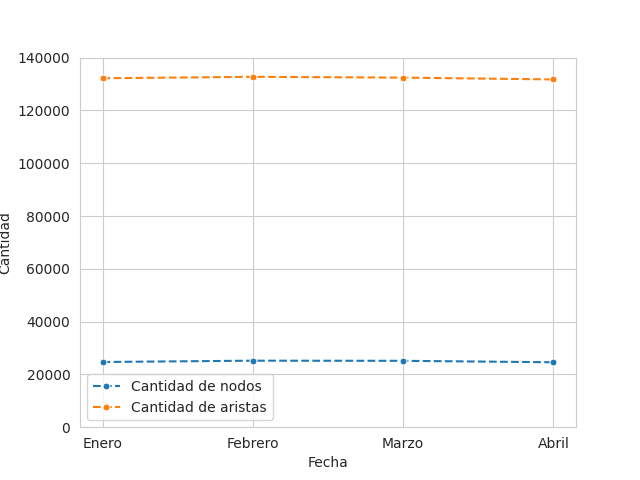
\includegraphics[width=0.7\textwidth]{img/resultados/cantidad_ases_rel_ribs.png}
%     \caption{Cantidad de relaciones y ASes para el primer día de los meses de enero, febrero, marzo y abril.}
%     \label{fig:cantidad_ases_rel_ribs}
% \end{figure}

\newpage
\begin{figure}[h]
    \centering
    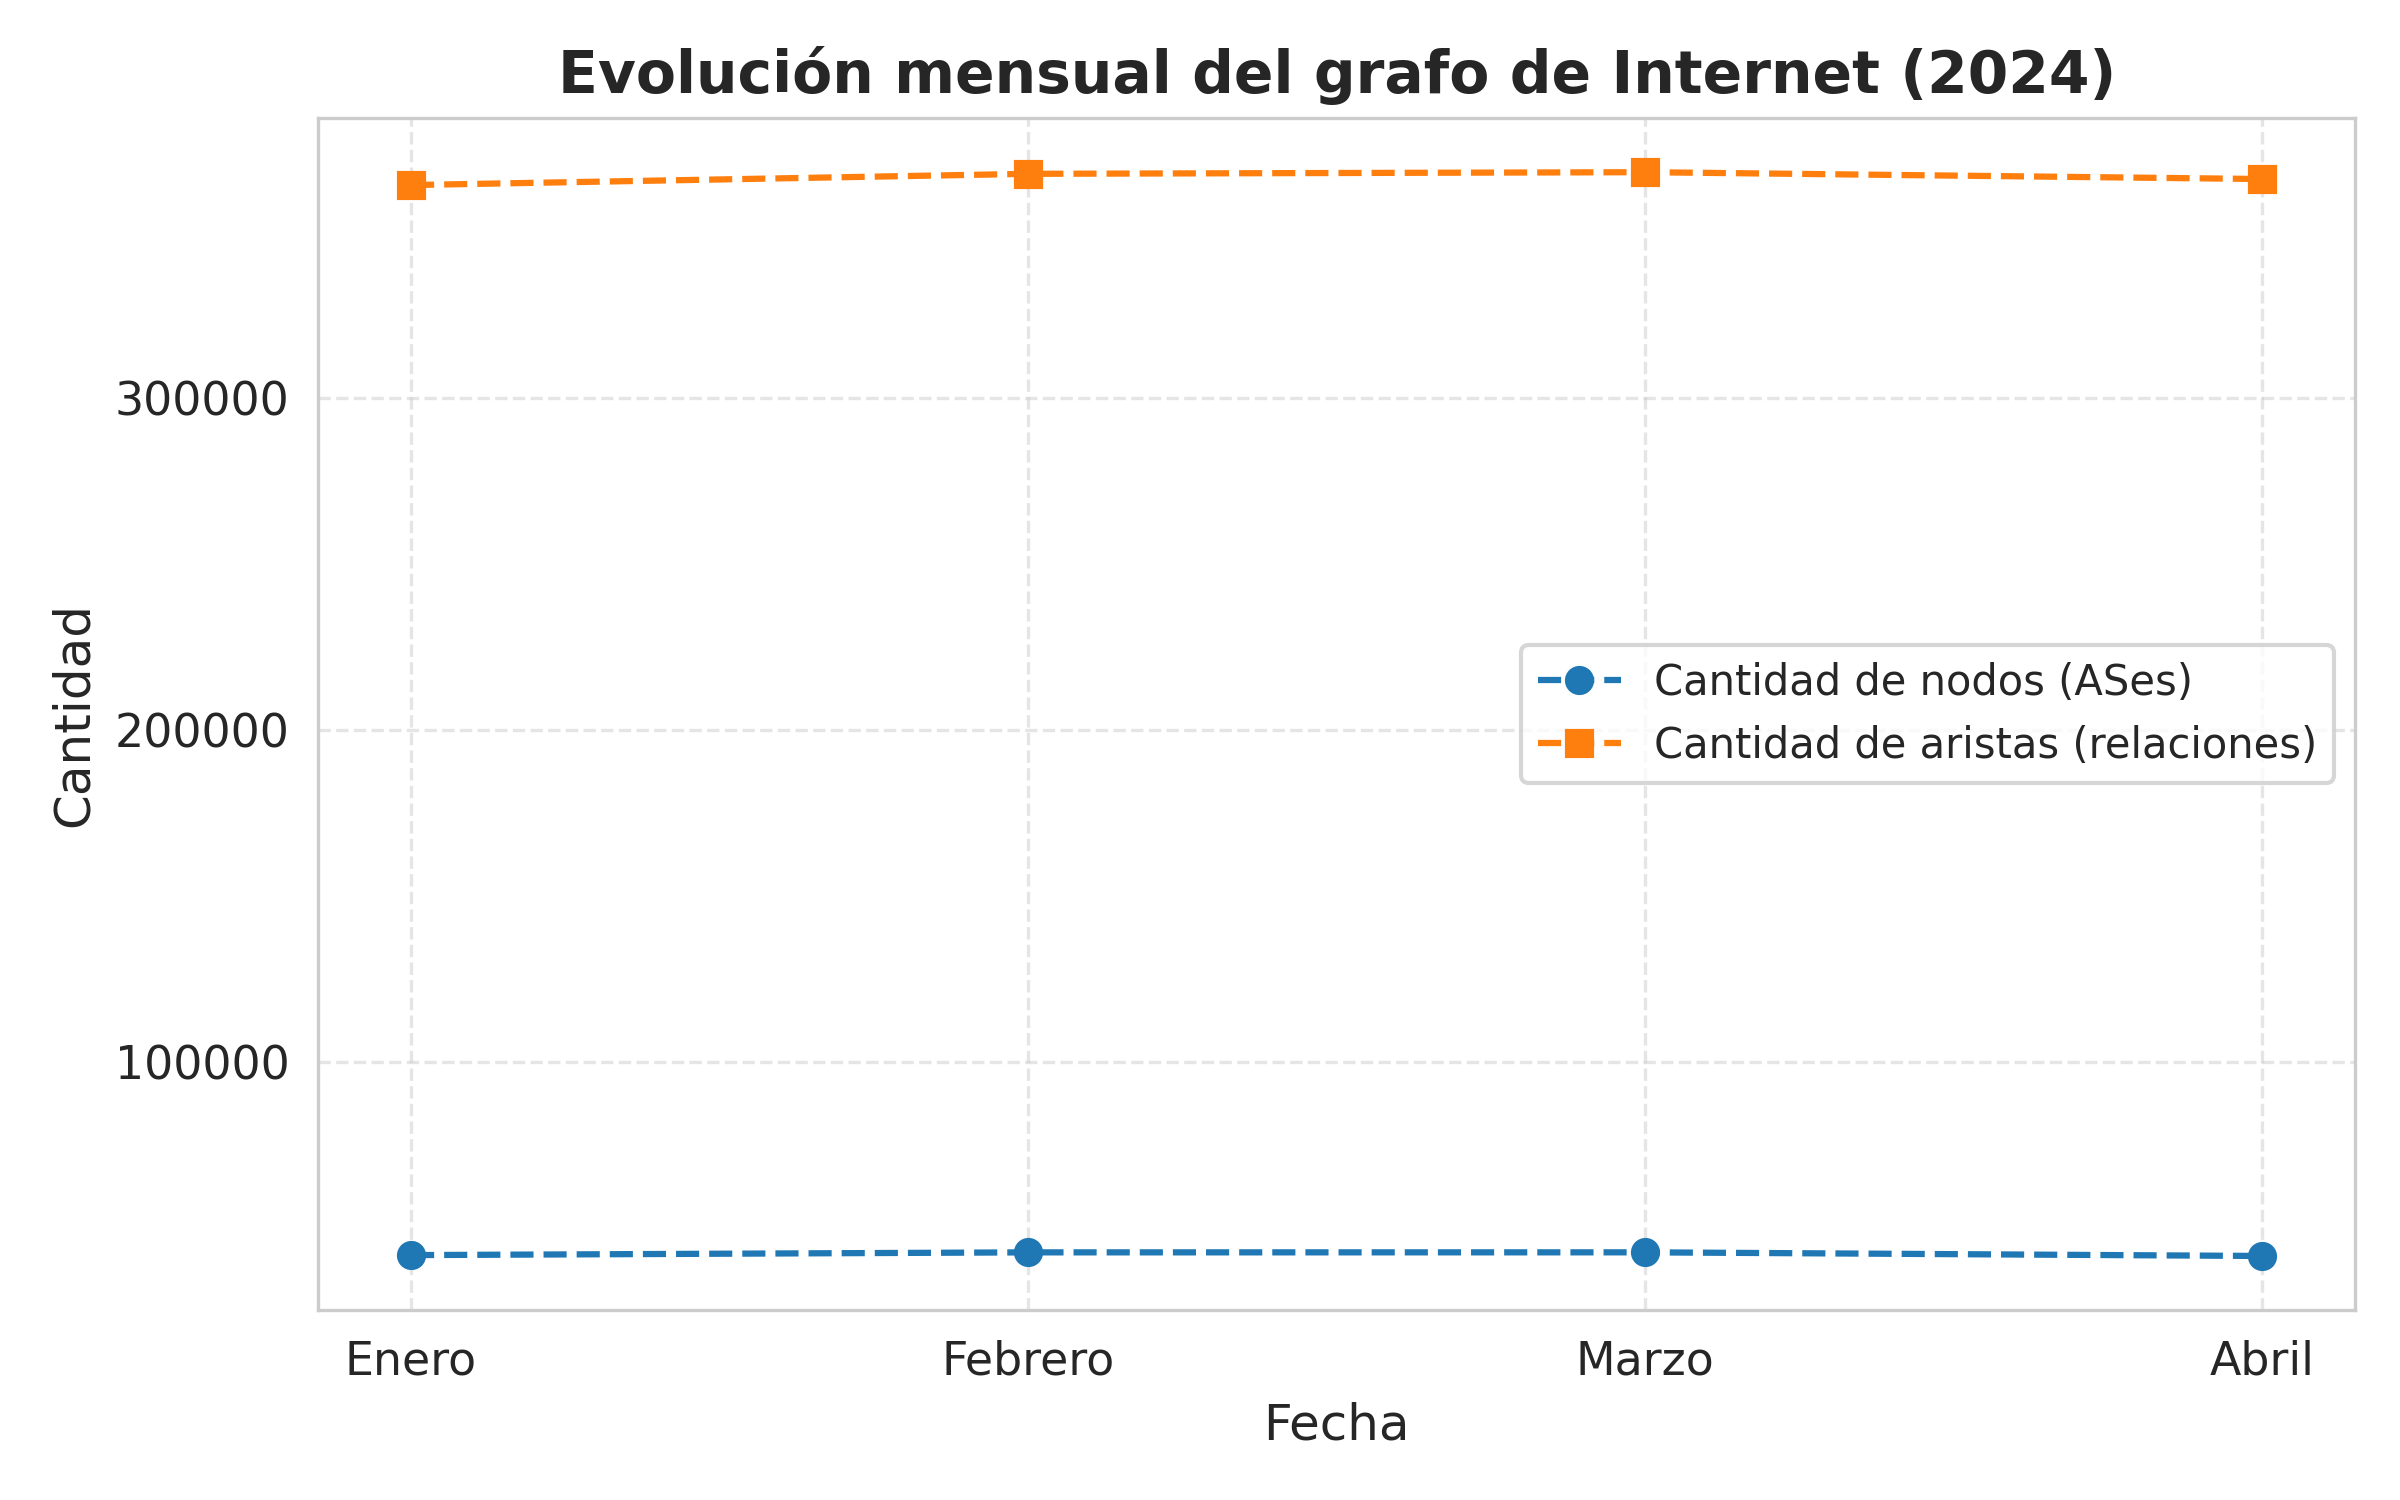
\includegraphics[width=0.9\textwidth]{img/resultados/cantidad_nodos_aristas_mensual.png}
    \caption{Cantidad de relaciones y ASes para los meses de enero a abril.}
    \label{fig:cantidad_nodos_aristas_mensual}
\end{figure}






% Para ver si utilizar únicamente las primeras 12 horas de cada mes generaba una pérdida de información, se extrajeron las RIBs correspondientes al día completo para los mismos meses. Esto permitió comparar la cantidad total de relaciones y ASes observados cuando se considera un mayor volumen de datos. Los resultados de esta comparación se presentan en la Figura~\ref{fig:cantidad_ases_rel_ribs_dia_completo}.

% \begin{figure}[H]
%     \centering
%     \includegraphics[width=0.9\textwidth]{img/resultados/cantidad_ases_rel_ribs_dia_completo.png}
%     \caption{.}
% \label{fig:cantidad_ases_rel_ribs_dia_completo}
% \end{figure}


% % TODO: Completar bien los datos
% \begin{table}[H]
%     \centering
%     \begin{tabular}{lcc}
%     \toprule
%     \textbf{Mes} & \textbf{Número de ASes} & \textbf{Número de Enlaces} \\
%     \midrule
%     Enero   &  24.696 & 227.260 \\ %FIX: Arrrgelar valor nodos
%     Febrero &  25.196 & 225.252 \\  %FIX: Arrrgelar valor nodos
%     Marzo   &  25.145 & 225.488 \\ %FIX: Arrrgelar valor nodos
%     Abril   &  26.543 & 226.541 \\ 
%     \end{tabular}
%     \caption{Cantidad de Ases y enlaces extraídos a partir de las RIBs extraídas.}
%     \label{tab:rib_datasets}
% \end{table}




\begin{table}[htbp]
\centering
\begin{tabular}{lrrrrrr}
\toprule
Mes & Nodos & Aristas & Densidad & Grado promedio & AS nuevos & AS retirados \\
\midrule
Enero    & 41.857 & 364.083 & 0.000208 & 8.70 & 0    & 0    \\
Febrero  & 42.683 & 367.470 & 0.000202 & 8.61 & 1.930 & 1.104 \\
Marzo    & 42.691 & 367.963 & 0.000202 & 8.62 & 211  & 203  \\
Abril    & 41.594 & 365.903 & 0.000212 & 8.80 & 1.213 & 2.310 \\
\bottomrule
\end{tabular}
\caption{Métricas mensuales extraídas de las RIBs BGP.}
\label{tab:caracteristicas_ribs_por_mes}
\end{table}


En la Tabla~\ref{tab:caracteristicas_ribs_por_mes} se observa la baja densidad de los grafos construidos a partir de las RIBs mensuales, la cual se mantiene en torno a 0.0002, lo cual es esperable en redes de gran escala como la de Internet, donde cada Sistema Autónomo se conecta a una fracción pequeña del total de nodos. Sin embargo, a pesar de la baja densidad, el grado promedio se mantiene estable entre 8.6 y 8.8, lo que sugiere que los ASes más relevantes continúan sosteniendo una conectividad considerable dentro de la red.\\




Para los fines de este trabajo, se consideraron como ASes Tier-1 a los siguientes: 174, 6461, 701, 1299, 3491, 3320, 6762, 7018, 12956, 6830, 6453, 5511, 3356, 3257, 2914, 2828, 1239, 286 y 209 (Para más información sobre estos ASes en la Tabla~\ref{tab:tier_1_ases} en el Anexo). La selección se basa en listas comúnmente aceptadas por la comunidad técnica~\cite{wikipedia_tier1}, las cuales identifican esos ASes como Tier-1 debido a su rol central en la infraestructura de Internet y la capacidad que tienen para llegar a cualquier destino sin pagar tránsito. Si bien no existe una definición oficial estricta, esta clasificación es usada ampliamente en estudios y repositorios públicos. En el contexto de este trabajo, fue necesario establecer este conjunto debido a que los métodos del \textit{benchmark} utilizan este listado para tomar decisiones de inferencia.



% Explicación siguientes grafos
En la Figura~\ref{fig:rel-tier1-ribs} se muestran las relaciones con al menos un AS Tier-1 en las RIBs recolectadas, mientras que la Figura~\ref{fig:rel-tier1} presenta el mismo análisis en AS Rank. Aunque AS Rank presenta una mayor cantidad de relaciones, en ambos casos se mantiene una proporción similar entre relaciones con y sin Tier-1, lo que podría indicar que nuestra extracción de RIBs conserva la estructura observada de Internet por AS Rank.\\


La diferencia en cantidad podría deberse al hecho de que las RIBs utilizadas corresponden a las primeras 12 horas del primer día de cada mes, lo que limita la visibilidad completa de las relaciones existentes. Esta restricción afecta principalmente a las relaciones entre ASes de niveles más bajos en la jerarquía de Internet, ya que estas suelen aparecer con menor frecuencia en las rutas BGP recolectadas. Por el contrario, las relaciones que involucran ASes Tier-1 las cuales tienen un rol más central en la infraestructura y por ende tienden a repetirse en múltiples rutas, ya que desde ellos es posible alcanzar cualquier otro punto de la red. En consecuencia, al capturar solo una fracción de las RIBs, se espera observar una menor proporción de relaciones que no incluyen ASes Tier-1.

\begin{figure}[ht]
    \centering
    
    \begin{subfigure}[b]{0.45\textwidth}
        \centering
        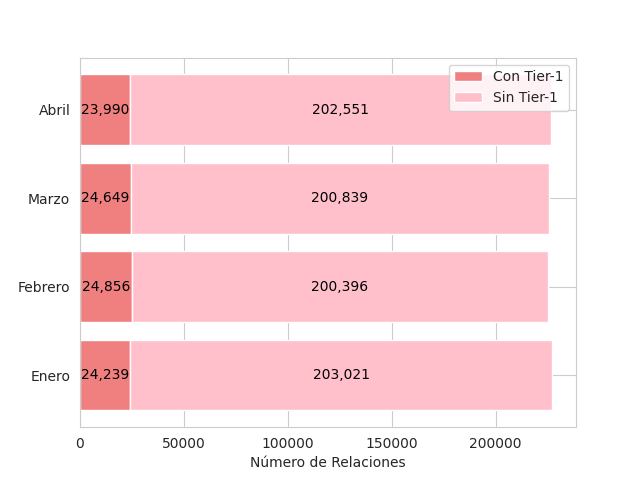
\includegraphics[width=\textwidth]{img/resultados/relaciones_con_tier1_ribs.png}
        \caption{Relaciones con al menos un AS Tier-1 en RIBs extraídas.}
        \label{fig:rel-tier1-ribs}
    \end{subfigure}
    \hfill
    \begin{subfigure}[b]{0.45\textwidth}
        \centering
        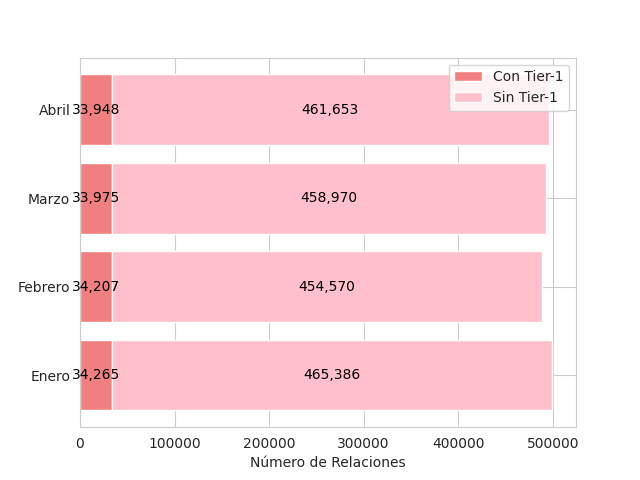
\includegraphics[width=\textwidth]{img/resultados/relaciones_con_tier1_asrank.png}
        \caption{Relaciones con al menos un AS Tier-1 en AS Rank.}
        \label{fig:rel-tier1}
    \end{subfigure}
    \caption{Comparación de relaciones que incluyen ASes Tier-1 entre RIBs recolectadas y AS Rank.}
\end{figure}

%Al analizar el grado de los ASes, es decir, la cantidad de conexiones directas que cada Sistema Autónomo (AS) mantiene con otros, es posible obtener una visión general de la estructura de conectividad en la red. Dado que las conexiones fueron extraídas de las RIBs, las cuales representan rutas hacia distintos destinos, se observa que todos los ASes tienen al menos una conexión de llegada (in-degree), pero no necesariamente una de salida (out-degree). Esto se debe a que cada ruta registrada en las RIBs describe un camino hacia un AS, lo que garantiza que cada uno de los ASes presentes haya sido alcanzado por al menos una ruta. \\



En las Figuras~\ref{fig:distribucion_as_grado_salida_entrada_febrero_boxplot_con_outliers} y \ref{fig:distribucion_as_grado_salida_febrero_boxplot_sin_outliers} se puede observar que son pocos los Sistemas Autónomos que cuentan con un número significativamente mayor de conexiones en comparación con el resto. Al graficar la distribución sin estos valores (outliers), resulta más fácil reconocer los cuartiles y comprender la dispersión de los datos, donde se aprecia que la mayoría de los ASes mantiene entre dos y cuatro relaciones salientes.
Esto se confirma en la Figura~\ref{fig:distribucion_as_grado_salida_entrada_febrero_log}, que muestra la distribución logarítmica del número de relaciones. En ella se evidencia una distribución de cola larga (\textit{long tail}), en la cual la gran mayoría de los ASes presenta un grado bajo, mientras que unos pocos concentran una cantidad desproporcionalmente alta  de conexiones. Este patrón es característico de redes jerárquicas  y sugiere que la topología AS-level de Internet sigue una distribución tipo ley de potencia (\textit{power-law}), donde un reducido número de nodos cumple un rol central de interconectividad.\\

\begin{figure}[H]
    \centering

    \begin{subfigure}[b]{0.48\textwidth}
        \centering
        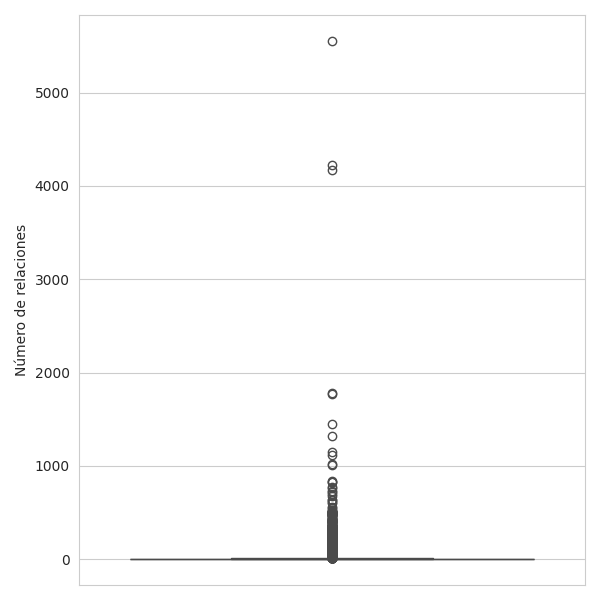
\includegraphics[width=\textwidth]{img/resultados/distribucion_as_grado_salida_febrero_boxplot_con_outliers.png}
        \caption{Distribucion de cantidad de aristas a un AS con outliers.}
        \label{fig:distribucion_as_grado_salida_entrada_febrero_boxplot_con_outliers}
    \end{subfigure}
    \hfill
    \begin{subfigure}[b]{0.48\textwidth}
        \centering
        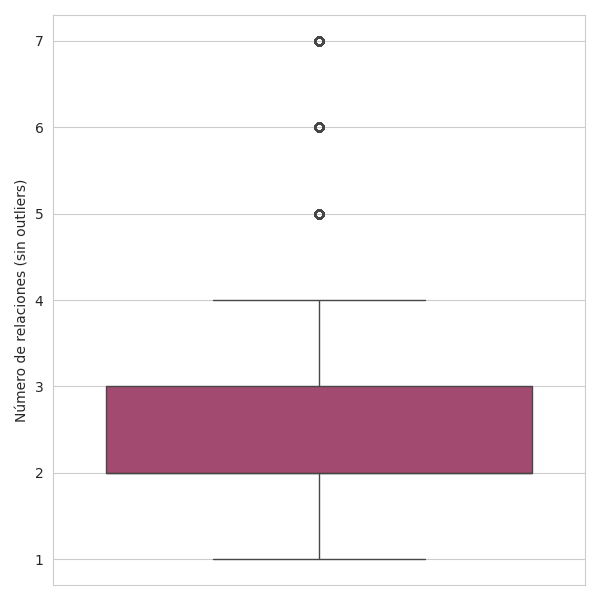
\includegraphics[width=\textwidth]{img/resultados/distribucion_as_grado_salida_entrada_febrero_boxplot_sin_outliers.png}
        \caption{Distribución de cantidad de aristas a un AS sin outliers.}
        \label{fig:distribucion_as_grado_salida_febrero_boxplot_sin_outliers}
    \end{subfigure}


    % Segunda fila: tercera subfigura
    \begin{subfigure}[b]{0.7\textwidth}
        \centering
        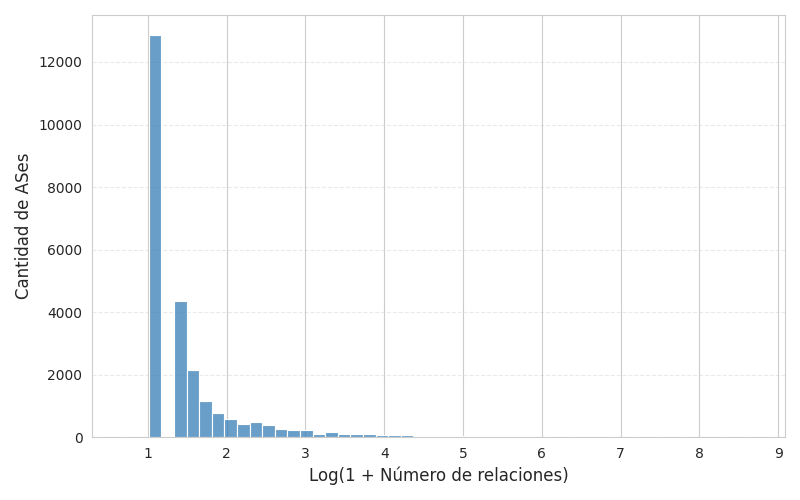
\includegraphics[width=\textwidth]{img/resultados/distribucion_as_grado_salida_entrada_febrero_log.png}
        \caption{Distribución en escala logarítmica.}
        \label{fig:distribucion_as_grado_salida_entrada_febrero_log}
    \end{subfigure}


    \caption{Comparación de la distribución del grado de salida de ASes en febrero, con y sin outliers.}
    \label{fig:distribucion_as_grado}
\end{figure}


%TODO: FIjarse mejor en como se quitaron los outliers (mencionarlo)




Además, en la Figura~\ref{fig:top_20_as_febrero_numerorelaciones} se presentan los 20 Sistemas Autónomos con mayor cantidad de conexiones. En el gráfico, los ASes son Tier-1 se destacan en un tono más oscuro. Como es de esperar, esto se debe a su rol central en la topología de Internet, lo que los hace más presentes en diferentes rutas y, por tanto, atractivos para que otros ASes establezcan conexiones con ellos. Esto reafirma lo establecido previamente, que la mayoría de ASes periféricos poseen menos presencia en rutas.\\



% TODO: Buscar paper donde hable de la jerarquia y estructura del Internet :)
% (Falta decir que los otros son tipo CArrier)
\begin{figure}[t]
    \centering
    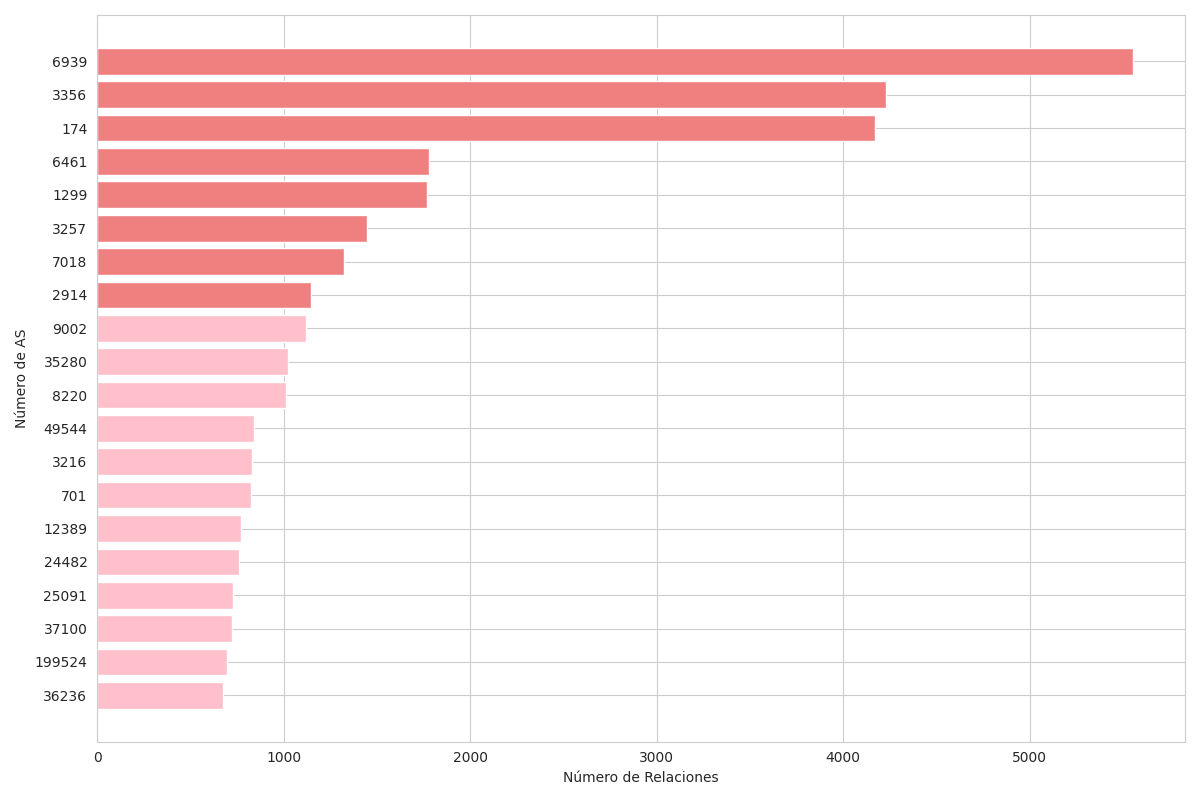
\includegraphics[width=0.7\textwidth]{img/resultados/top_20_as_febrero_numerorelaciones_src.png}
    \caption{Top 20 ASes con mayor número de conexiones (grado), para RIB de febrero 2024.}
\label{fig:top_20_as_febrero_numerorelaciones}
\end{figure}



Otro análisis que se realizó fue graficar la distribución de la longitud de las rutas BGP observadas en las RIBs (Figura~\ref{fig:distribucion_largo_path}), donde se observa una clara concentración en longitudes entre 3 y 5 Sistemas Autónomos, siendo la longitud más frecuente de 4 saltos. Esta distribución sugiere una estructura de red eficiente, donde la mayoría de los destinos pueden ser alcanzados con pocos saltos intermedios. Además, la ausencia de rutas de longitud 1 y valores atípicos evidentes, indican que el proceso de limpieza y filtrado de las rutas fue hecho de buena  manera y sin errores evidentes. Figura~\ref{fig:comparacion_mensual_largo_paths} en el Anexo presenta una comparación de esta distribución entre los distintos meses analizados.\\

\begin{figure}[H]
    \centering
    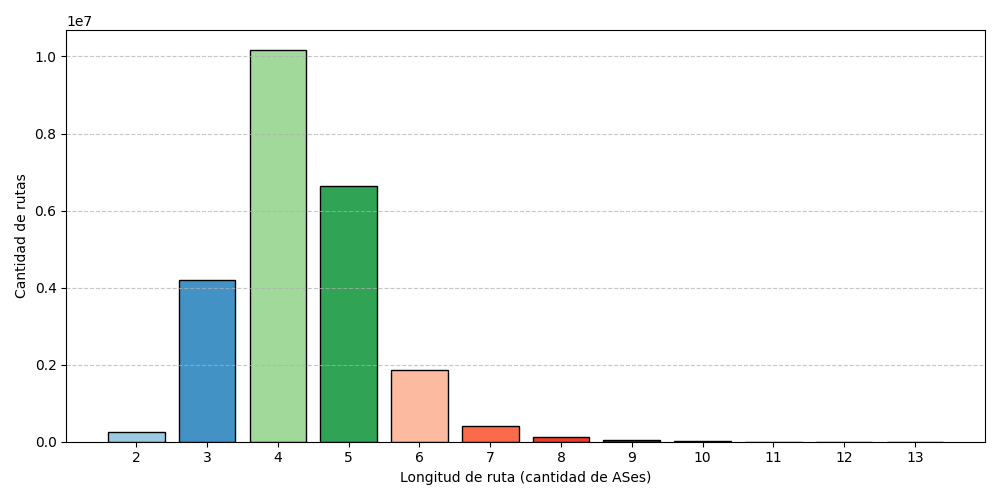
\includegraphics[width=0.7\textwidth]{img/resultados/distribucion_largo_paths.png}
    \caption{Distribución de longitud de rutas BGP.}
\label{fig:distribucion_largo_path}
\end{figure}


En la misma línea, se analizó la frecuencia con la que los ASes aparecen en las rutas BGP extraídas. Permitiendo identificar ASes que ocupan posiciones centrales dentro de la infraestructura de Internet, al participar en un gran número de caminos de enrutamiento.\\

Figura~\ref{fig:top_20_as_febrero_numerorelaciones} presenta el top 20 de Sistemas Autónomos con mayor frecuencia de aparición en las rutas BGP extraídas. Los ASes con mayor grado y por ende más conectados están destacados en color naranja. Esto refuerza la idea del rol central que desempeñan los ASes de nivel Tier-1 en la infraestructura de Internet, al combinar una alta conectividad (alto grado de conectividad) con una participación recurrente en múltiples trayectorias (alta frecuencia de aparición de múltiples caminos), evidenciando su importancia en el enrutamiento.\\


\begin{figure}[H]
    \centering
    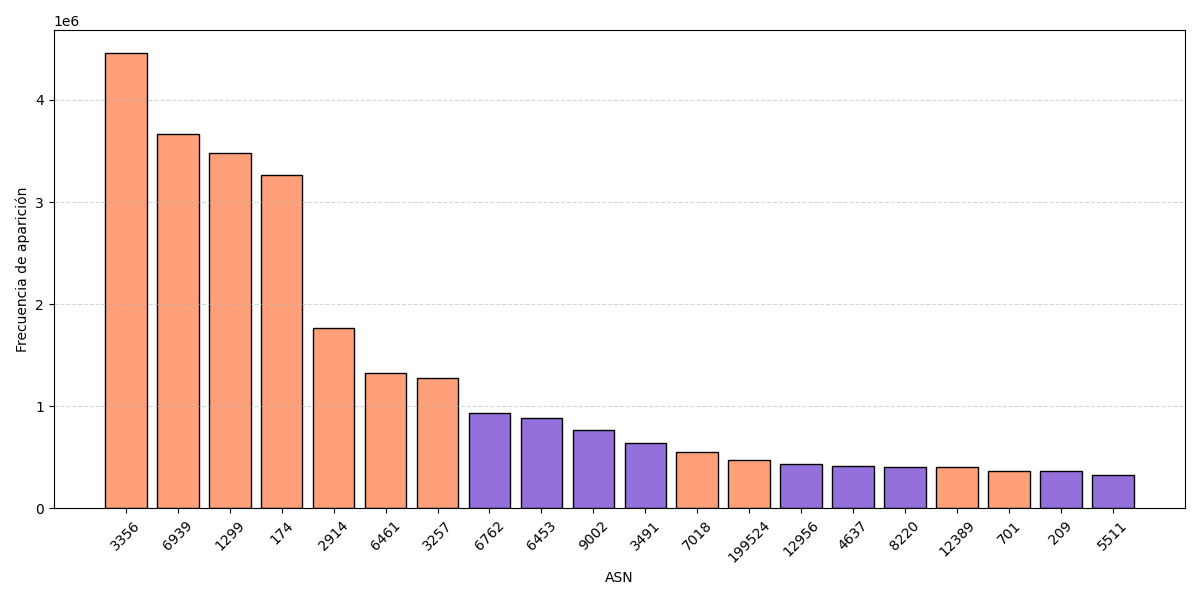
\includegraphics[width=0.8\textwidth]{img/resultados/top_20_ases_frecuencia_ribs.png}
    \caption{Top 20 ASes más frecuentes en rutas BGP (Febrero 2024).}
\label{fig:top_20_ases_frecuencia_ribs}
\end{figure}



% COMIENZO ANALICIS AS RANK ---------------------------------------------------------

%DATASET ASRANK\\

%\vspace{1cm}
\paragraph{Dataset ASRank}

%\vspace{1cm}

Para la evaluación y entrenamiento, de los métodos del \textit{benchmark} se utilizó ASRank, el cual contiene aproximadamente 76.000 Sistemas Autónomos y 499.651 enlaces. En la Tabla~\ref{tab:asrank_datasets}, ubicada en el Anexo~\ref{sec:attr_asrank_section}, se detalla la cantidad de conexiones y ASes correspondientes a los cuatro primeros meses.\\

Para complementar esta información, en la Figura~\ref{fig:cantidad_asrank_meses}  se presenta la evolución mensual del número de ASes y enlaces registrados por ASRank y la cantidad de cada tipo de relación.\\

\begin{figure}[H]
    \centering

    \begin{subfigure}[h]{0.4\textwidth}
        \centering
        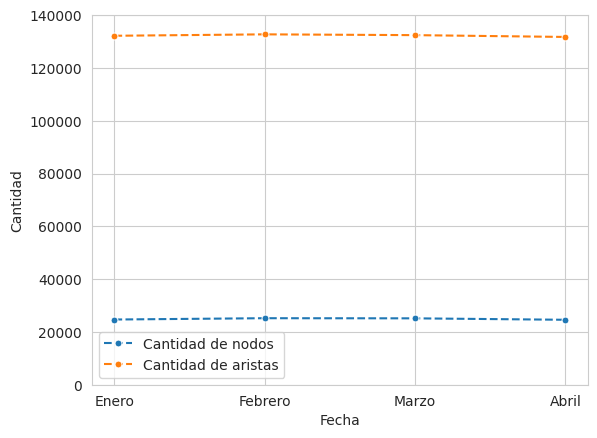
\includegraphics[width=\textwidth]{img/resultados/ribs/cantidad_nodos_aristas_por_fechaUntitled.png}
        \caption{Cantidad de ASes y relaciones extraídas de las RIBs.}
        \label{fig:cantidad_nodos_aristas_por_fecha_ribs}
    \end{subfigure}
    \hfill
    \begin{subfigure}[h]{0.50\textwidth}
        \centering
        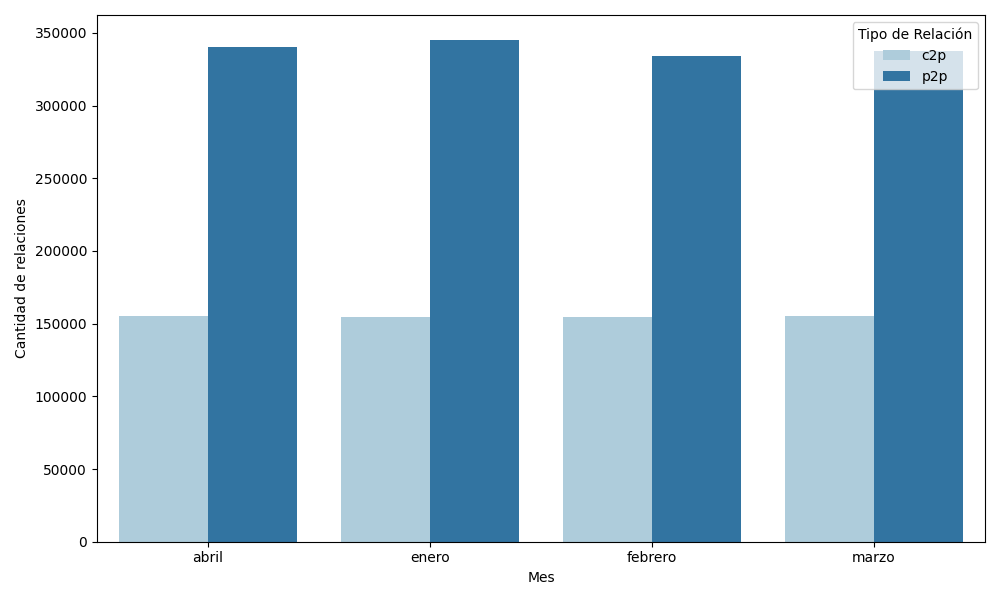
\includegraphics[width=\textwidth]{img/resultados/asrank/relaciones_por_tipo_asrank.png}
        \caption{Cantidad de relaciones por tipo según AS Rank.}
        \label{fig:relaciones_por_tipo_asrank}
    \end{subfigure}

    \caption{Cantidad de ASes, relaciones y tipos de relaciones de AS Rank para los meses de enero a abril de 2024.}
    \label{fig:cantidad_asrank_meses}
\end{figure}

\newpage
Los ASes con más relaciones C2P son en su mayoría Tier-1, como Cogent (AS174) y Lumen (AS3356), reflejando su rol como proveedores de tránsito. En contraste, los ASes con más relaciones P2P incluyen tanto Tier-1 como actores regionales o de hosting, como i3D.net (AS49544). La Tabla~\ref{tab:info_ases_top} entrega información complementaria sobre cada AS, permitiendo entender su rol en la estructura global de Internet.\\


\begin{figure}[H]
    \centering
    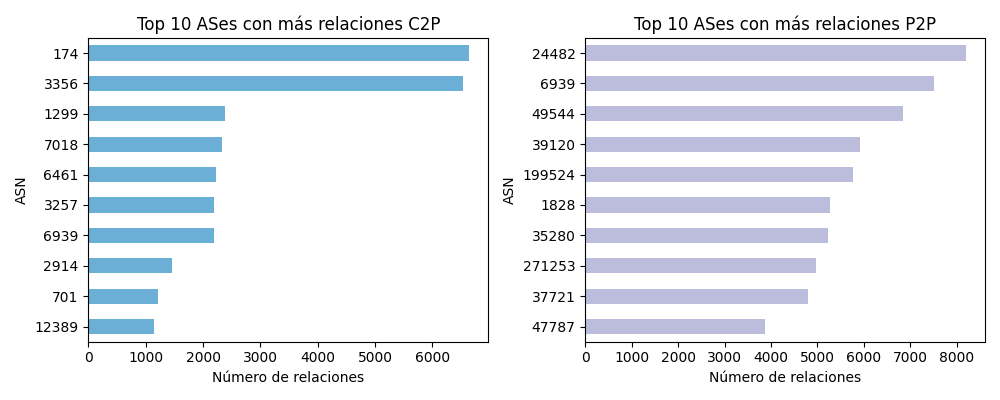
\includegraphics[width=0.9\textwidth]{img/resultados/top_ases_por_tipo_relacion.png}
    \caption{Top 10 ASes con mayor cantidad de relaciones C2P y P2P inferidas}
    \label{fig:top_ases_relaciones}
\end{figure}



Otro análisis consistió en comparar la cantidad de Sistemas Autónomos y aristas coincidentes entre los PATHs recolectados desde las RIBs y los presentes en el dataset de AS Rank. Esta comparación fue importante, ya que luego el dataset de AS Rank se ocupó para etiquetar los enlaces presentes en la topología. En la Figura~\ref{fig:aristas_coincidentes_por_mes_con_ribs} se muestra la cantidad de coincidencias de ASes y aristas por mes.\\


\begin{figure}[H]
    \centering
    \begin{subfigure}[h]{0.40\textwidth}
        \centering
        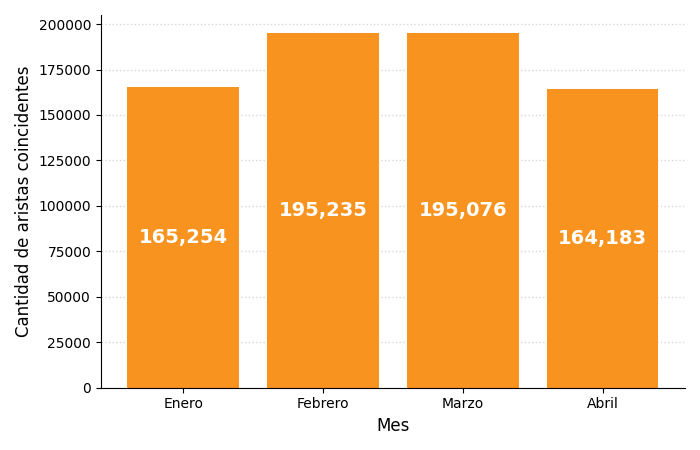
\includegraphics[width=\textwidth]{img/resultados/aristas_coincidentes_por_mes_con_ribs.png}
        \caption{Aristas coincidentes entre AS paths extraídos de las RIBs y de AS Rank.}
        \label{fig:aristas_coincidentes_por_mes_con_ribs}
    \end{subfigure}
    \hfill
    \begin{subfigure}[h]{0.40\textwidth}
        \centering
        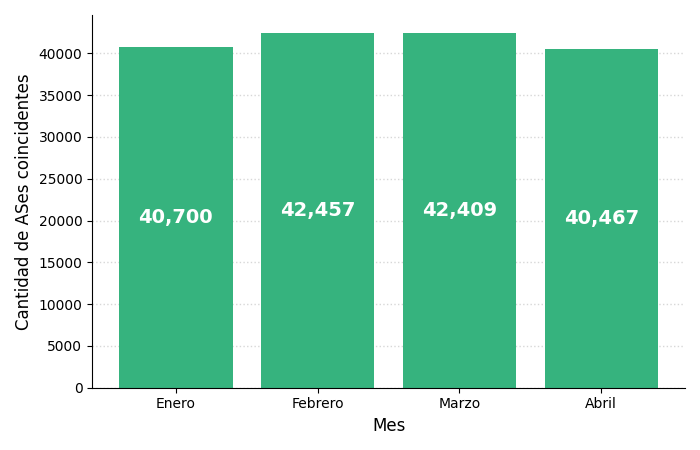
\includegraphics[width=\textwidth]{img/resultados/ases_coincidentes_por_mes_ribs.png}
        \caption{ASes coincidentes entre AS paths extraídos de las RIBs y de AS Rank.}
        \label{fig:ases_coincidentes_por_mes_ribs}
    \end{subfigure}
    \caption{Comparación de coincidencias entre RIBs recolectadas y AS Rank.}
    \label{fig:coincidencias_ribs_asrank}
\end{figure}



\begin{table}[H]
\centering
\caption{Información y clasificación de los principales ASes observados.}
\label{tab:info_ases_top}
\resizebox{\textwidth}{!}{
\begin{tabular}{lll}
\toprule
\textbf{ASN} & \textbf{Organización} & \textbf{Rol / Tipo} \\
\midrule
174     & Cogent Communications        & Tier-1 ISP           \\
3356    & Level 3 / Lumen              & Tier-1 ISP           \\
1299    & Arelion (ex Telia)           & Tier-1 ISP           \\
7018    & AT\&T Services               & Tier-1 ISP           \\
6461    & Zayo Group                   & Tier-1 ISP           \\
3257    & GTT Communications           & Tier-1 ISP           \\
6939    & Hurricane Electric           & Tier-1 ISP           \\
2914    & NTT America                  & Tier-1 ISP           \\
701     & Verizon Business             & Tier-1 ISP           \\
12389   & Rostelecom                   & Tier-1 nacional      \\
\midrule
24482   & SG.GS (Singapur)             & Hosting / Peer       \\
49544   & i3D.net (Holanda)            & Gaming / Hosting     \\
39120   & Consoltech (Europa del Este) & Datacenter           \\
199524  & MivoCloud (Moldavia)         & ISP regional         \\
1828    & Telenor (Noruega)            & ISP nacional         \\
35280   & Omantel                      & ISP nacional         \\
271253  & Empresa Argentina de Soluciones Satelitales (ARSAT) & ISP nacional \\
37721   & Safaricom (Kenia)            & ISP nacional         \\
47787   & Hosting Ukraine Ltd          & Hosting / Peer       \\
\bottomrule
\end{tabular}
}
\end{table}



%/////////////////////////////////////////////////
%/////////////////////////////////////////////////
%/////////////////////////////////////////////////
\vspace{0.5cm}
\section{Resultados del uso de Redes Neuronales de Grafos (GNNs)} \label{sec:gnn_result_section}

Como se mencionó previamente, para el uso de modelos GNN se exploraron dos enfoques: el \textbf{entrenamiento \textit{por etapas}} (Sección~\ref{sec:resultados_entrenamiento_por_etapas}) y el \textbf{entrenamiento \textit{end-to-end}} (Sección~\ref{sec:entrenamiento_end_to_end}).
A continuación se presenta una descripción de los experimentos y sus respectivos resultados.\\

%Las métricas utilizadas para evaluar los modelos se definen a continuación. 
%La \textbf{Accuracy} corresponde a la exactitud global, calculada como la proporción de instancias correctamente clasificadas sobre el total de ejemplos. 
%Por otro lado, las métricas de \textbf{Precision} y \textbf{Recall} se reportan como \textit{micro-promedio}, es decir, considerando de manera conjunta los verdaderos positivos (TP), falsos positivos (FP) y falsos negativos (FN) de todas las clases como si se tratara de un único problema binario, para luego aplicar las fórmulas correspondientes:

%\[
%\text{Precision}_{micro} = \frac{\sum_{i=1}^C TP_i}{\sum_{i=1}^C (TP_i + FP_i)}
%\]

%\[
%\text{Recall}_{micro} = \frac{\sum_{i=1}^C TP_i}{\sum_{i=1}^C (TP_i + FN_i)}
%\]

%\[
%\text{Accuracy} = \frac{\sum_{i=1}^C TP_i}{\sum_{i=1}^C (TP_i + FP_i + FN_i + TN_i)}
%\]

%donde \(C\) corresponde al número de clases consideradas.

%/////////////////////////////////////////////////

\subsection{Resultados de Entrenamiento \textit{Por Etapas}} \label{sec:resultados_entrenamiento_por_etapas}

En este enfoque, el aprendizaje se divide en dos fases separadas: primero se generan \textit{embeddings} para cada nodo del grafo, y luego estos \textit{embeddings} se utilizan como entrada para un modelo de clasificación. El flujo de trabajo fue el siguiente:


\begin{enumerate}
    \item Importación de RIBs y construcción del grafo DGL.
    \item Asociación de atributos a cada nodo, siguiendo los mismos tres casos mencionados anteriormente.
    \item Generación de representaciones vectoriales para cada AS mediante un modelo GNN entrenado para una tarea auxiliar. Se evaluaron dos estrategias principales:
    \begin{itemize}
        \item Inferencia de la existencia de conexiones entre nodos (tarea de predicción de enlaces).
        \item Inferencia de características específicas de los ASes a partir de su contexto en el grafo (por ejemplo, clasificación o clustering).
    \end{itemize}
    \item Uso de los \textit{embeddings} obtenidos como entrada para un modelo MLP que predice la relación entre pares de ASes.
\end{enumerate}

Dado el desbalance de clases en el dataset, en todos los experimentos se evaluaron con y sin balance de clases, así como con entrenamiento con el grafo completo y por batches. Además, cada caso fue probado utilizando los tres tipos de encoder (GCN, GraphSAGE y GAT) y ambos decoders (MLP y producto punto), para ver su comportamiento.\\

A continuación, se presentan los diferentes experimentos creados con este enfoque.\\



%/////////////////////////////////////////////////
\subsubsection{Caso 0: Predicción de enlaces utilizando grafo con atributos de nodos extraídos de PeeringDB}

\begin{itemize}
    \item \textbf{RIBs:} Febrero 2024.
    \item \textbf{Atributos de nodos:} Dataset creado a partir de PeeringDB.
   \item \textbf{Tarea para la creación de \textit{embeddings}:} Determinar la existencia o no de un enlace entre pares de nodos (Sistemas Autónomos).
    \item \textbf{Tamaño \textit{embeddings}:} 32.
    \item \textbf{Epochs:} 100 (GNN) y 20 (ANN).
    \item \textbf{Early Stopping:} Paciencia de 8 epochs.
    \item \textbf{Learning Rate:} 0.001 (GNN) y 0,001 (ANN).
\end{itemize}




% decir q se crearon aristas grafo ngativo

A continuación, los resultados obtenidos a partir de la tarea para crear \textit{embeddings}. La Tabla~\ref{tab:comparacion_accuracy_caso0} resume los valores de AUC y Accuracy alcanzados por cada combinación de encoder y decoder, mientras que la Figura \ref{fig:partes_caso_0_comparacion_roc_auc} presenta las curvas ROC asociadas, lo que permite contrastar visualmente el desempeño de cada variante.\\

\begin{figure}[H]
    \centering
    % Primera fila
    \begin{subfigure}[b]{0.45\textwidth}
        \centering
        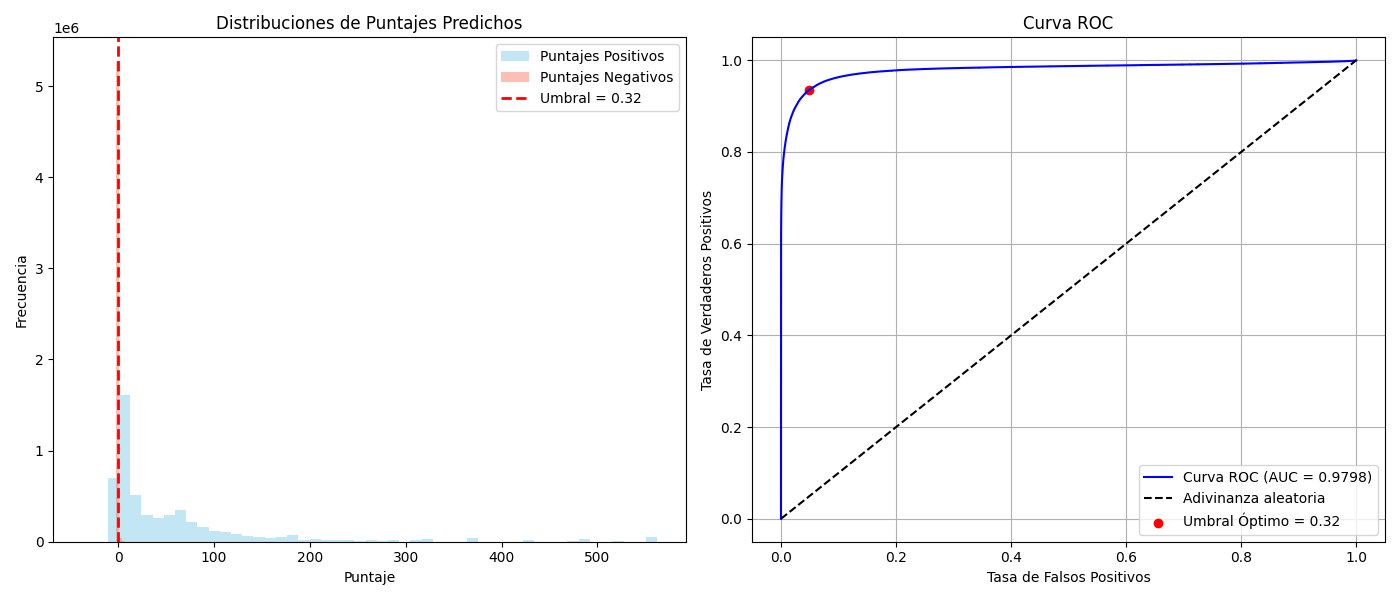
\includegraphics[width=\textwidth]{img/resultados/gnn/partes/caso2_mis_attr/resultados/roc_curve_GCN_DotProduct_mis_attr_febrero.png}
        \caption{GCN + Producto Punto}
        \label{fig:conf_matrix_gcn_dp}
    \end{subfigure}
    \hfill
    \begin{subfigure}[b]{0.45\textwidth}
        \centering
        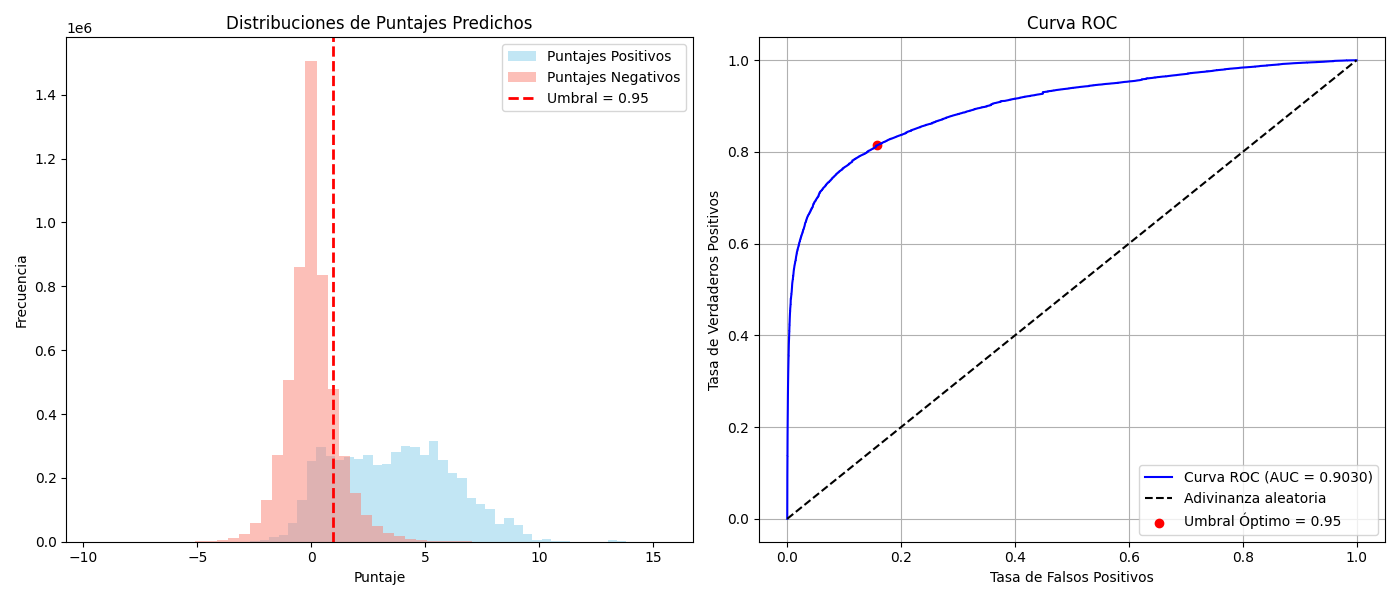
\includegraphics[width=\textwidth]{img/resultados/gnn/partes/caso2_mis_attr/resultados/roc_curve_GraphSAGE_DotProduct_mis_attr_febrero.png}
        \caption{GraphSAGE + Producto Punto}
        \label{fig:conf_matrix_sage_dp}
    \end{subfigure}

    \vspace{0.5cm}

    % Segunda fila
    \begin{subfigure}[b]{0.45\textwidth}
        \centering
        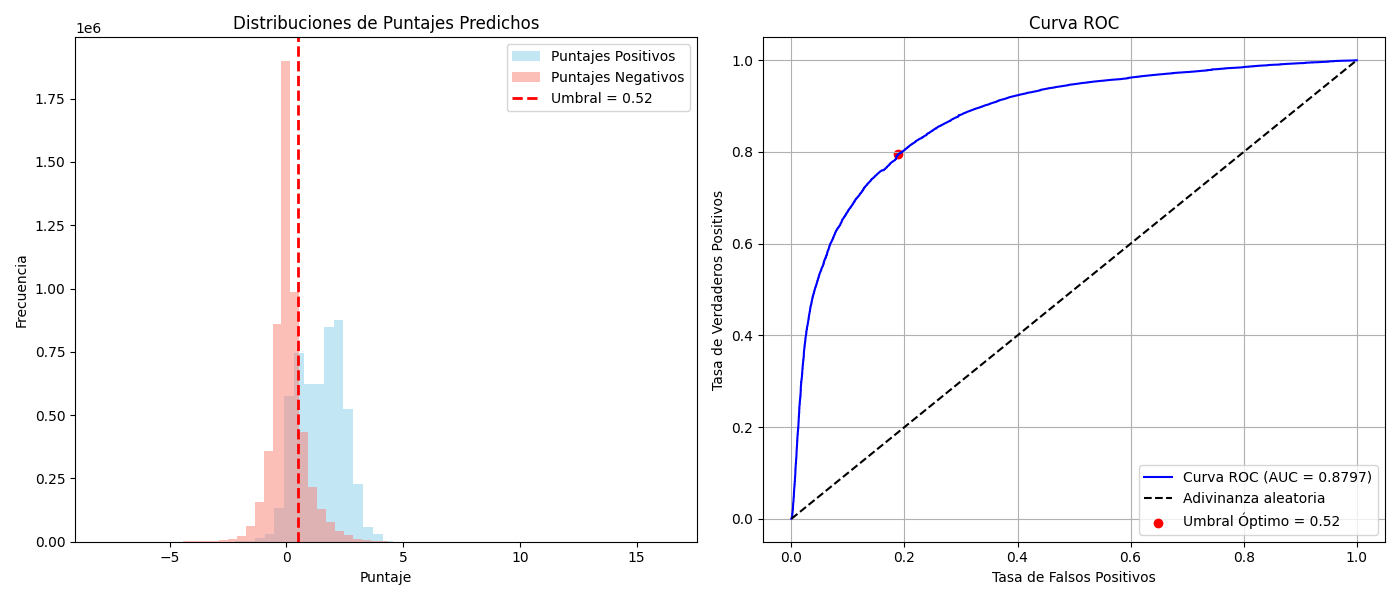
\includegraphics[width=\textwidth]{img/resultados/gnn/partes/caso2_mis_attr/resultados/roc_curve_GAT_DotProduct_mis_attr_febrero.png}
        \caption{GAT + Producto Punto}
        \label{fig:conf_matrix_gat_dp}
    \end{subfigure}
    \hfill
    \begin{subfigure}[b]{0.45\textwidth}
        \centering
        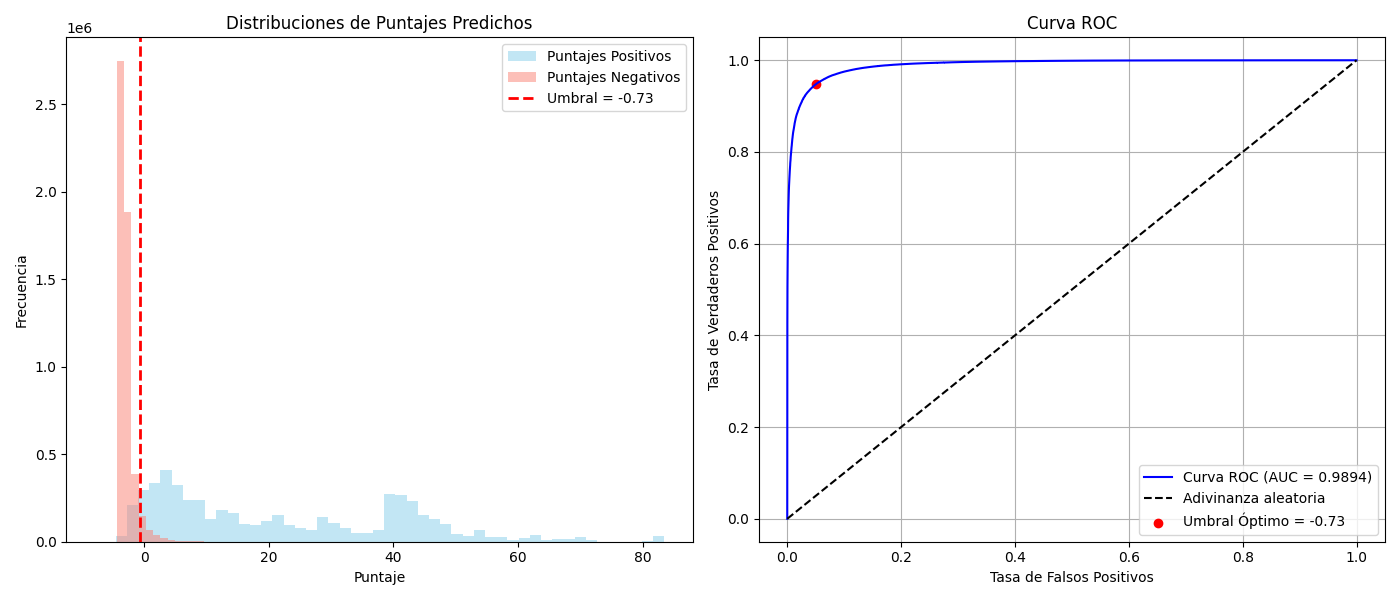
\includegraphics[width=\textwidth]{img/resultados/gnn/partes/caso2_mis_attr/resultados/roc_curve_GCN_MLP_mis_attr_febrero.png}
        \caption{GCN + MLP}
        \label{fig:conf_matrix_gcn_mlp}
    \end{subfigure}

    \vspace{0.5cm}

    % Tercera fila
    \begin{subfigure}[b]{0.45\textwidth}
        \centering
        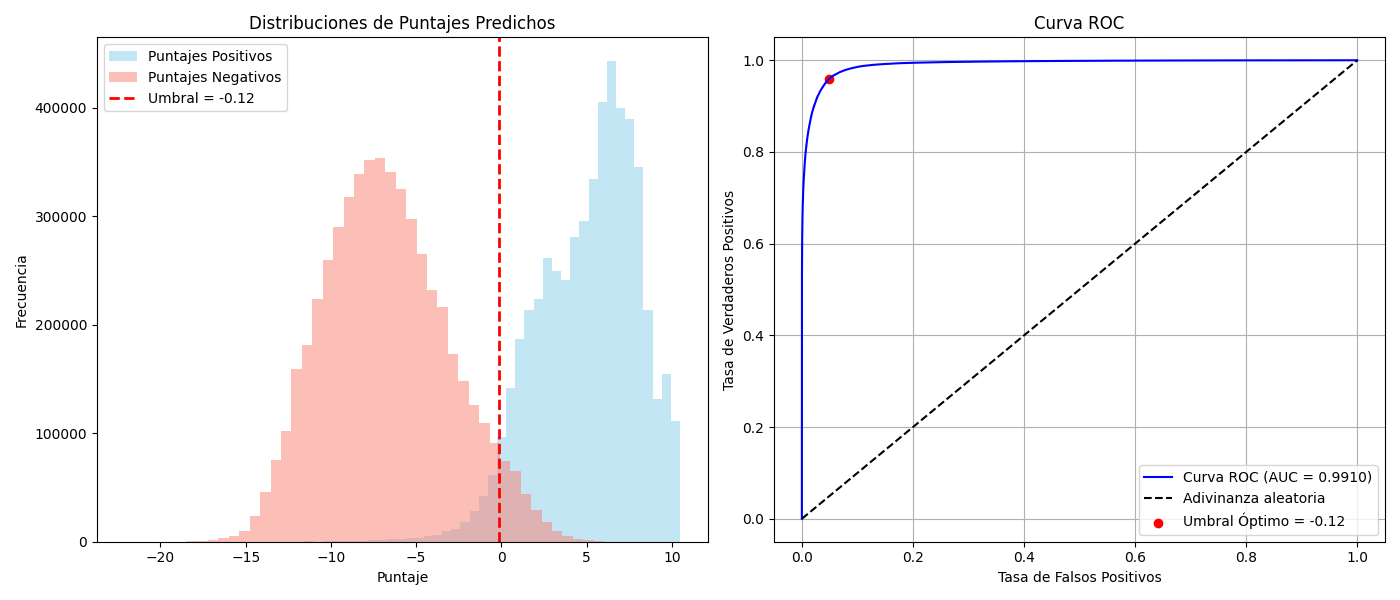
\includegraphics[width=\textwidth]{img/resultados/gnn/partes/caso2_mis_attr/resultados/roc_curve_GraphSAGE_MLP_mis_attr_febrero.png}
        \caption{\textbf{GraphSAGE + MLP}}
        \label{fig:conf_matrix_sage_mlp}
    \end{subfigure}
    \hfill
    \begin{subfigure}[b]{0.45\textwidth}
        \centering
        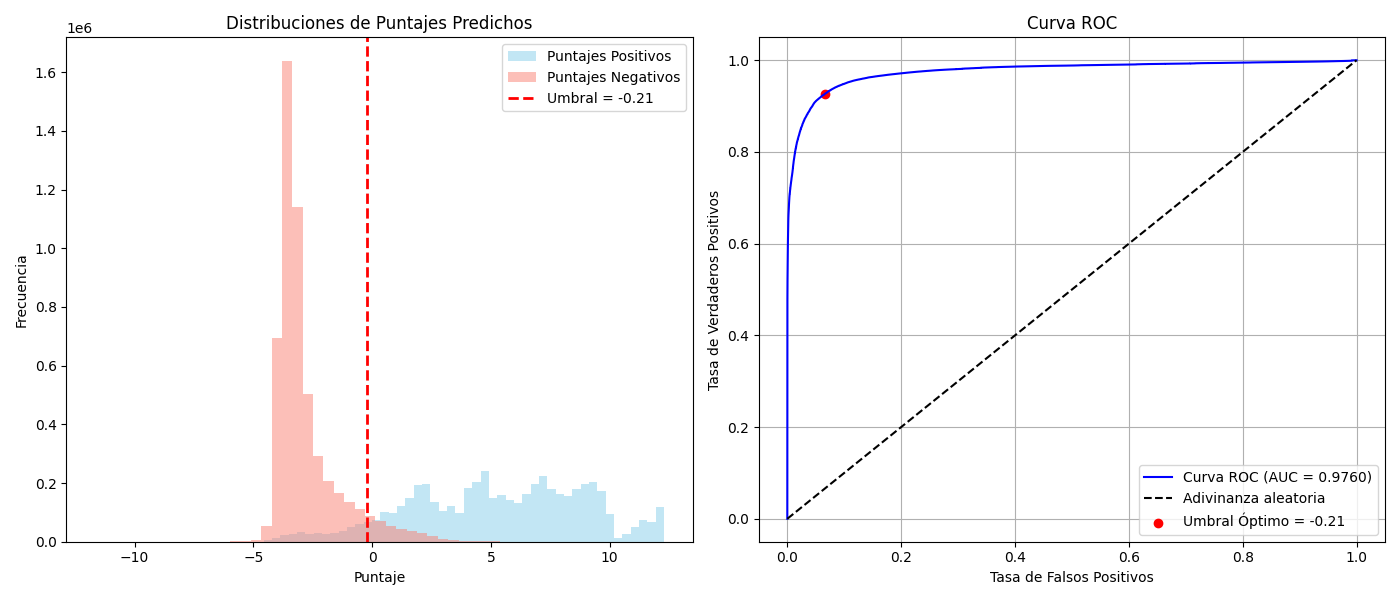
\includegraphics[width=\textwidth]{img/resultados/gnn/partes/caso2_mis_attr/resultados/roc_curve_GAT_MLP_mis_attr_febrero.png}
        \caption{GAT + MLP}
        \label{fig:conf_matrix_gat_mlp}
    \end{subfigure}

    \caption{Curvas ROC y distribución de los resultados.}
    \label{fig:partes_caso_0_comparacion_roc_auc}
\end{figure}

En todos los modelos (GCN, GraphSAGE y GAT), el decodificador MLP supera a Dot Product. Esto sugiere que un decodificador más expresivo es capaz de capturar mejor las relaciones entre los ASes. En contraste, el Dot Product es un decodificador simple que solo mide la “similitud” entre vectores, lo que puede resultar insuficiente para esta tarea.



\begin{table}[H]
    \centering
    \begin{tabular}{lccc}
    \hline
    \textbf{Modelo} & \textbf{Decodificador} & \textbf{AUC}& \textbf{Accuracy (\%)} \\
    \hline
    GCN & Dot Product &  0.986 & 0.945 \\
    GraphSAGE & Dot Product & 0.913 &  0.835\\
    GAT & Dot Product & 0.887 & 0.840 \\
    GCN & MLP  & 0.991 & 0.952 \\
    \textbf{GraphSAGE} & \textbf{MLP}  & \textbf{0.991} & \textbf{0.958} \\
    GAT & MLP &  0.967 & 0.916 \\
    \hline
    \end{tabular}
    \caption{Accuracy de la inferencia con link prediction para la creación de \textit{embeddings}.}
    \label{tab:comparacion_accuracy_caso0}
\end{table}

\newpage
Luego de la generación de \textit{embeddings}, se evaluó la tarea principal. En la Tabla~\ref{tab:accuracy_gnn_variants_caso0} se muestran los resultados de Accuracy obtenidos para cada combinación de encoder y decoder. Las cuales consisten en: sin batching y sin balanceo (`NoBatch-NoW'), sin batching pero con balanceo (`NoBatch-W'), con batching sin balanceo (`Batch-NoW'), y con ambas (`Batch-W').  \\


\begin{table}[H]
\centering
\resizebox{\textwidth}{!}{%
\begin{tabular}{llcccccccccccc}
\toprule
\multirow{2}{*}{\textbf{Modelo}} & 
\multirow{2}{*}{\textbf{Decodificador}} & 
\multicolumn{3}{c}{\textbf{NoBatch-NoW}} & 
\multicolumn{3}{c}{\textbf{NoBatch-W}} & 
\multicolumn{3}{c}{\textbf{Batch-NoW}} & 
\multicolumn{3}{c}{\textbf{Batch-W}} \\
\cmidrule(lr){3-5} \cmidrule(lr){6-8} \cmidrule(lr){9-11} \cmidrule(lr){12-14}
 & & \textbf{Precision} & \textbf{Recall} & \textbf{Accuracy} 
   & \textbf{Precision} & \textbf{Recall} & \textbf{Accuracy} 
   & \textbf{Precision} & \textbf{Recall} & \textbf{Accuracy} 
   & \textbf{Precision} & \textbf{Recall} & \textbf{Accuracy} \\
\midrule
GCN       & Dot Product &82.57&75.93&79.57&79.56&64.07&73.35&84.84&78.99&82.07&76.00&61.17&70.22\\
GraphSAGE & Dot Product &\textbf{86.08}&\textbf{83.87}&\textbf{85.04}&81.71&72.59&77.95&85.58&83.03&84.35&81.04&75.48&78.73\\
GAT       & Dot Product &85.83&81.69&83.80&79.98&71.85&76.53&86.10&83.62&84.94&79.94&73.36&77.00\\
\midrule
GCN       & MLP         &73.18&69.59&71.74&75.50&16.30&50.47&71.68&71.03&71.45&73.64&18.93&51.78\\
GraphSAGE & MLP         &82.33&76.82&79.75&79.39&53.34&70.44&78.74&74.05&76.74&76.75&44.08&65.82\\
GAT       & MLP         &79.97&74.04&77.27&64.04&38.26&60.57&76.08&71.47&74.30&66.56&32.81&59.56\\
\bottomrule
\end{tabular}}
\caption{Resultados de Precision, Recall y Accuracy (\%) por combinación de encoder y decoder bajo cuatro configuraciones: sin batching y sin balanceo (`NoBatch-NoW'), sin batching con balanceo (`NoBatch-W'), con batching sin balanceo (`Batch-NoW'), y con ambas (`Batch-W'). En negrita se indican los mejores resultados por métrica en cada configuración.}
\label{tab:accuracy_gnn_variants_caso0}
\end{table}

Podemos ver que se obtienen los mejores resultados con GraphSAGE y Dot Product como decoder, con una Accuracy de 85.04\%, diferente a lo que es de esperar, ya que para la creación de los \textit{embeddings}, con el decodificador MLP se obtuvieron los mejores resultados.\\

Esto ocurre porque para la clasificación de tipos de relación (C2P, P2P, P2C) con una ANN, lo que más importa es que los \textit{embeddings} sean bien estructurados y fáciles de separar. Aquí, el decoder Dot Product tiende a generar \textit{embeddings} más simples, lo que termina beneficiando la tarea final. Por otro lado, el NoBatch es mejor en rendimiento porque la ANN siempre entrena con la distribución global de los datos.\\


Se utilizó balanceo de clases aplicando pesos a cada categoría. Esto por el desbalance del dataset donde la clase mayoritaria es P2P, lo que podría sesgar al modelo y aumentar de forma falsa la Accuracy, ya que “acierta” muchos casos P2P únicamente por su alta frecuencia. Luego, la Precision y Recall de P2P tienden a ser altas, pero para C2P y P2C (las minorías) tienden a ser más bajas (Recall no las detecta y Precision confunde con P2P).


%Al observar los resultados de la Tabla~\ref{tab:accuracy_gnn_variants_caso0} y la Figura~\ref{fig:anex:matrices_confusion_experimentos_gnns_decoder}, se aprecia claramente el impacto del balanceo de clases (weights) en el desempeño. Cuando no se aplica balanceo, se observa una fuerte predominancia hacia la clase P2P, lo que indica que el modelo tiende a predecir mayoritariamente este tipo de enlace, independientemente de la clase real. Sin embargo, la tabla de accuracies muestra que el valor de accuracy es más alto cuando no se aplica balanceo, lo que puede resultar engañoso. Esto se debe a que la métrica de accuracy considera solo la proporción de aciertos globales y no penaliza la distribución desigual entre clases.\\

%En cuanto al uso de batching, su efecto no es tan pronunciado, sin embargo, en ciertos casos se observa una ligera mejora en la identificación de clases minoritarias al utilizar batching.\\

%Por último, al comparar con BGP2Vec, se observa que este método no se ve tan afectado por el desbalance de clases, a pesar de que la misma red neuronal (ANN) se utiliza como tarea downstream. Esto sugiere que los embeddings generados mediante GNNs son más sensibles al desbalance, ya que durante el proceso de message passing se refuerza la información de los enlaces dominantes, induciendo un sesgo en las representaciones aprendidas y afectando la capacidad del modelo para discriminar correctamente las clases minoritarias.  



% Se utilizaron un millón de rutas AS\_PATHS para construir el grafo de Internet. A partir de este grafo, se aplicaron diversas arquitecturas GNNs para generar los embeddings correspondientes. Los resultados obtenidos pueden ser consultados en el Anexo~\ref{sec:anexo_por_partes_caso_2}.\\


\subsubsection{Caso 1: Predicción de enlaces utilizando grafo con atributos de grado de entrada y salida}


\begin{itemize}
    \item \textbf{RIBs:} Febrero 2024.
    \item \textbf{Atributos de nodos:} Grado de entrada y salida de cada nodo.
    \item \textbf{Tarea para la creación de \textit{embeddings}:}  Determinar la existencia o no de un enlace entre pares de nodos (Sistemas Autónomos).
    \item \textbf{Tamaño \textit{embeddings}:} 32.
    \item \textbf{Epochs:} 100 (GNN) y 20 (ANN).
    \item \textbf{Early Stopping:} Paciencia de 8 epochs.
    \item \textbf{Learning Rate:} 0.001 (GNN) y 0,001 (ANN). 
\end{itemize}



A continuación se presentan los resultados obtenidos a partir de la tarea para crear \textit{embeddings}. La Tabla \ref{tab:accuracy_gnn_full} resume los valores de AUC y Accuracy alcanzados por cada combinación de encoder y decoder, mientras que la Figura \ref{fig:comparacion_roc_auc_caso1_full} presenta las curvas ROC asociadas, lo que permite contrastar visualmente el desempeño de cada variante.\\


\begin{figure}[H]
    \centering
    % Primera fila ── GCN
    \begin{subfigure}[b]{0.45\textwidth}
        \centering
        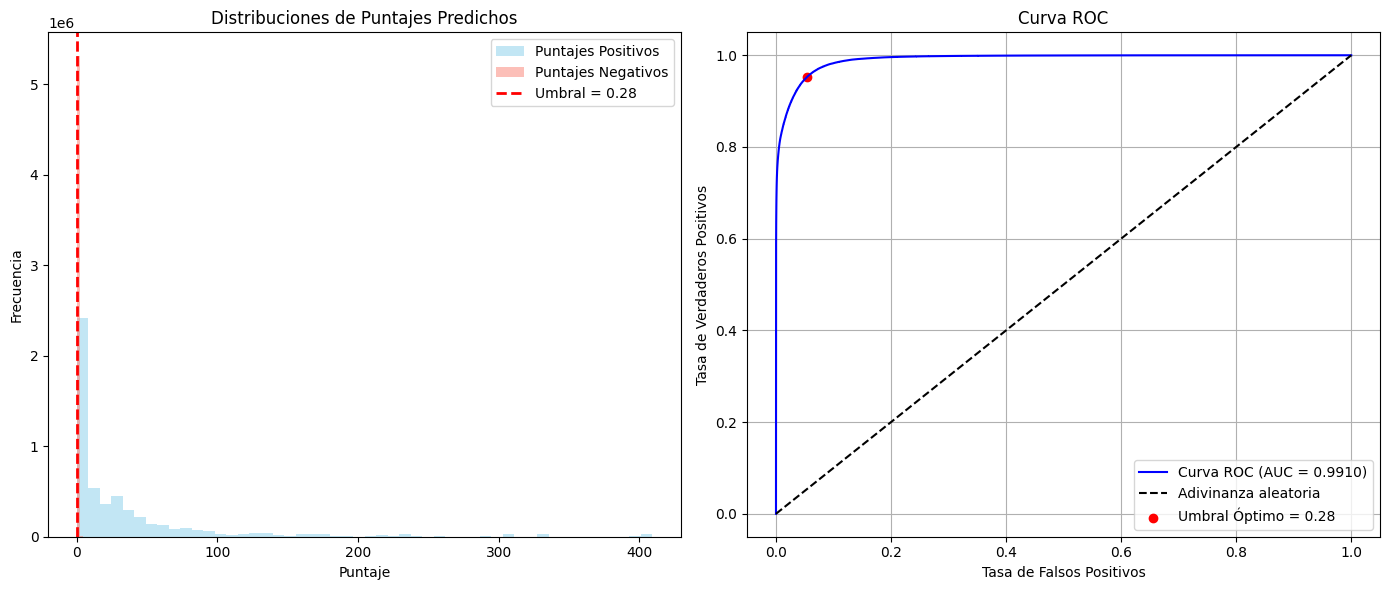
\includegraphics[width=\textwidth]{img/resultados/gnn/partes/caso1_degree/full/roc_GCN_DP_full.png}
        \caption{GCN + Dot Product}
        \label{fig:roc_gcn_dp_full}
    \end{subfigure}
    \hfill
    \begin{subfigure}[b]{0.45\textwidth}
        \centering
        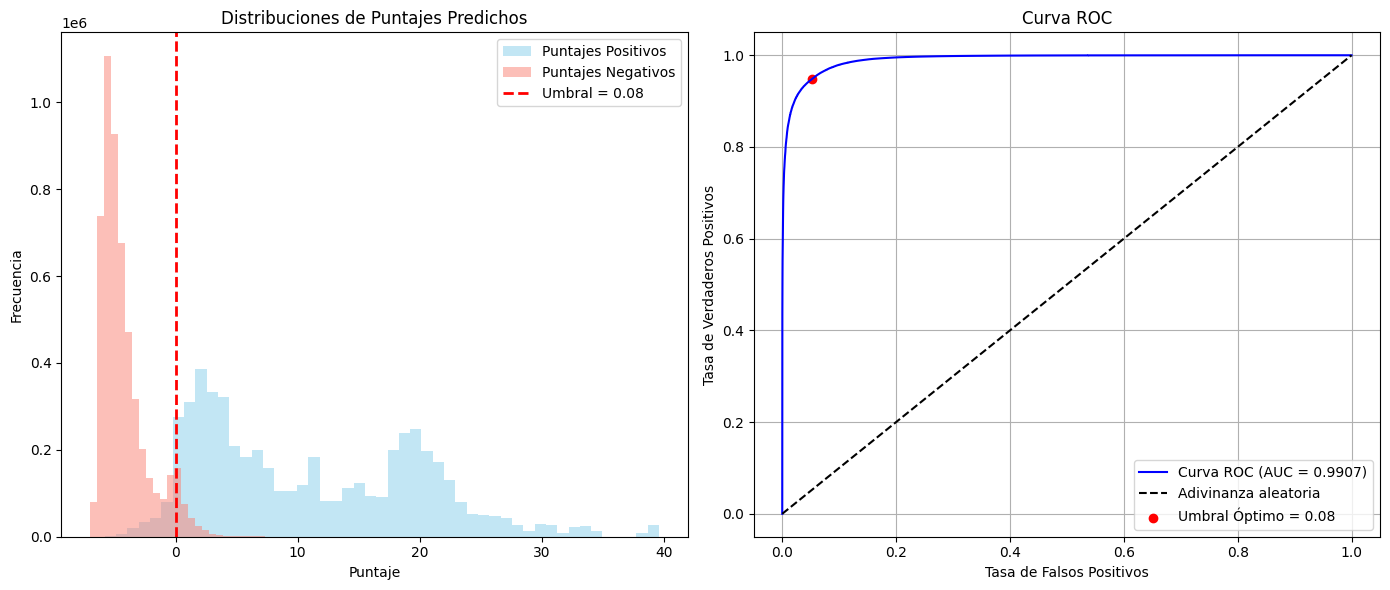
\includegraphics[width=\textwidth]{img/resultados/gnn/partes/caso1_degree/full/roc_GCN_MLP_full.png}
        \caption{GCN + MLP}
        \label{fig:roc_gcn_mlp_full}
    \end{subfigure}

    \vspace{0.5cm}

    % Segunda fila ── GraphSAGE
    \begin{subfigure}[b]{0.45\textwidth}
        \centering
        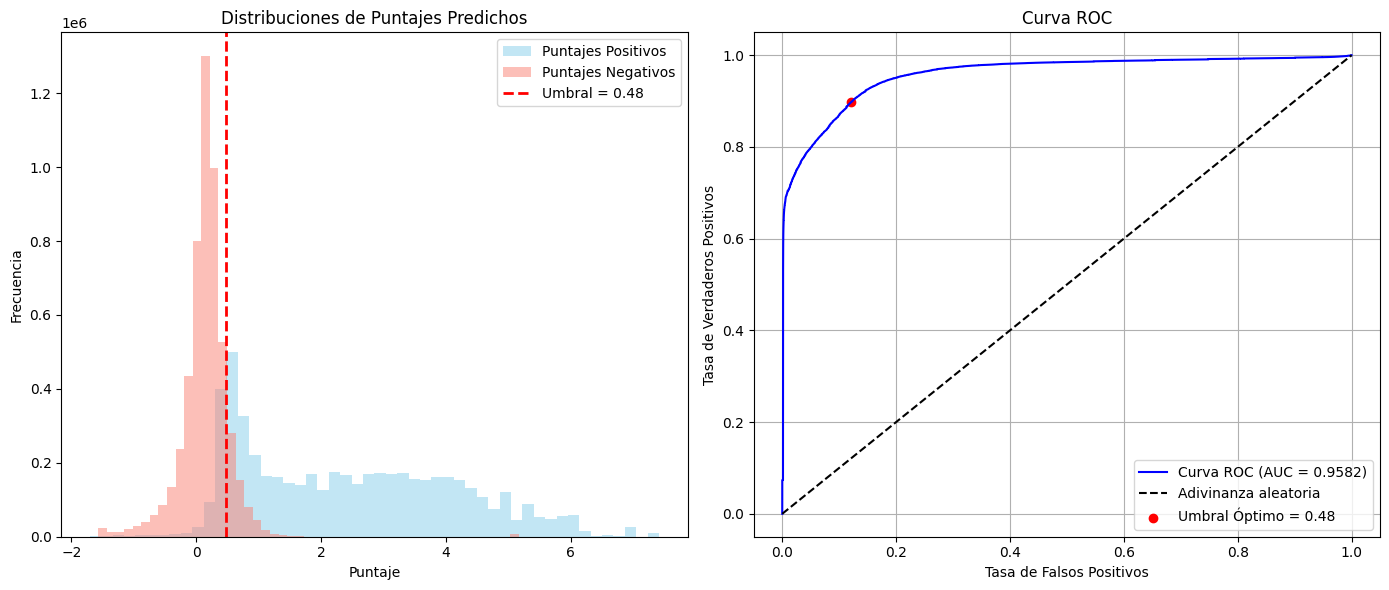
\includegraphics[width=\textwidth]{img/resultados/gnn/partes/caso1_degree/full/roc_GraphSAGE_DP_full.png}
        \caption{GraphSAGE + Dot Product}
        \label{fig:roc_graphsage_dp_full}
    \end{subfigure}
    \hfill
    \begin{subfigure}[b]{0.45\textwidth}
        \centering
        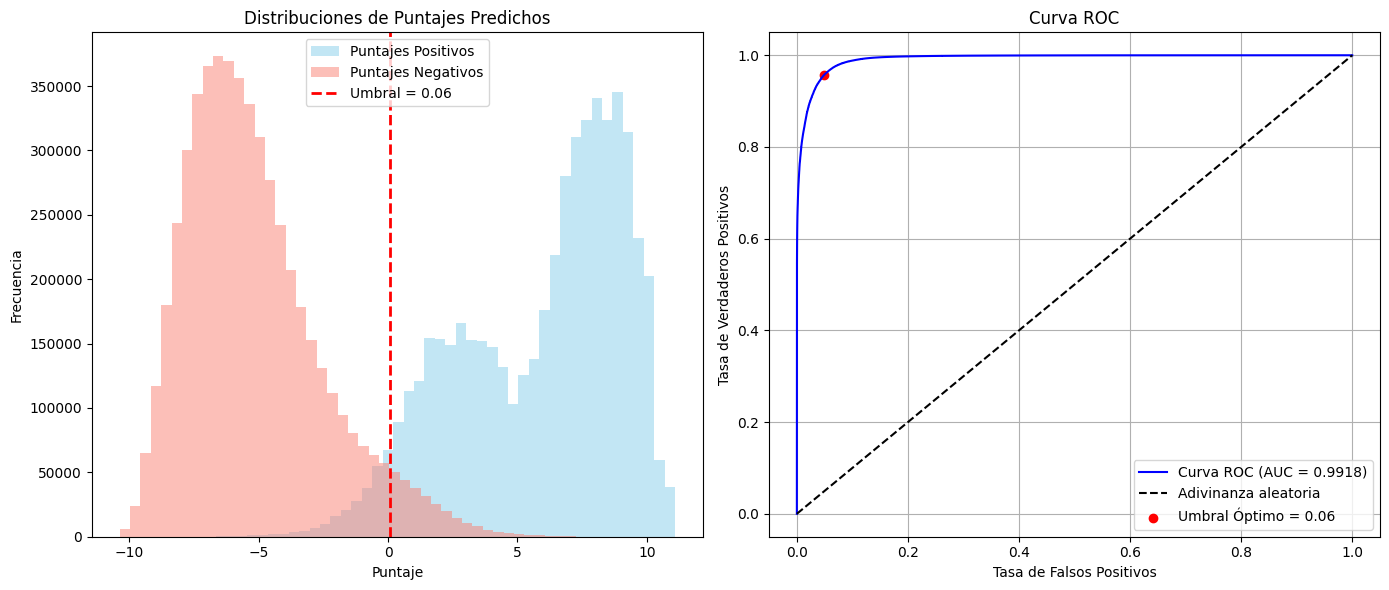
\includegraphics[width=\textwidth]{img/resultados/gnn/partes/caso1_degree/full/roc_GraphSAGE_MLP_full.png}
        \caption{\textbf{GraphSAGE + MLP}}
        \label{fig:roc_graphsage_mlp_full}
    \end{subfigure}

    \vspace{0.5cm}

    % Tercera fila ── GAT
    \begin{subfigure}[b]{0.45\textwidth}
        \centering
        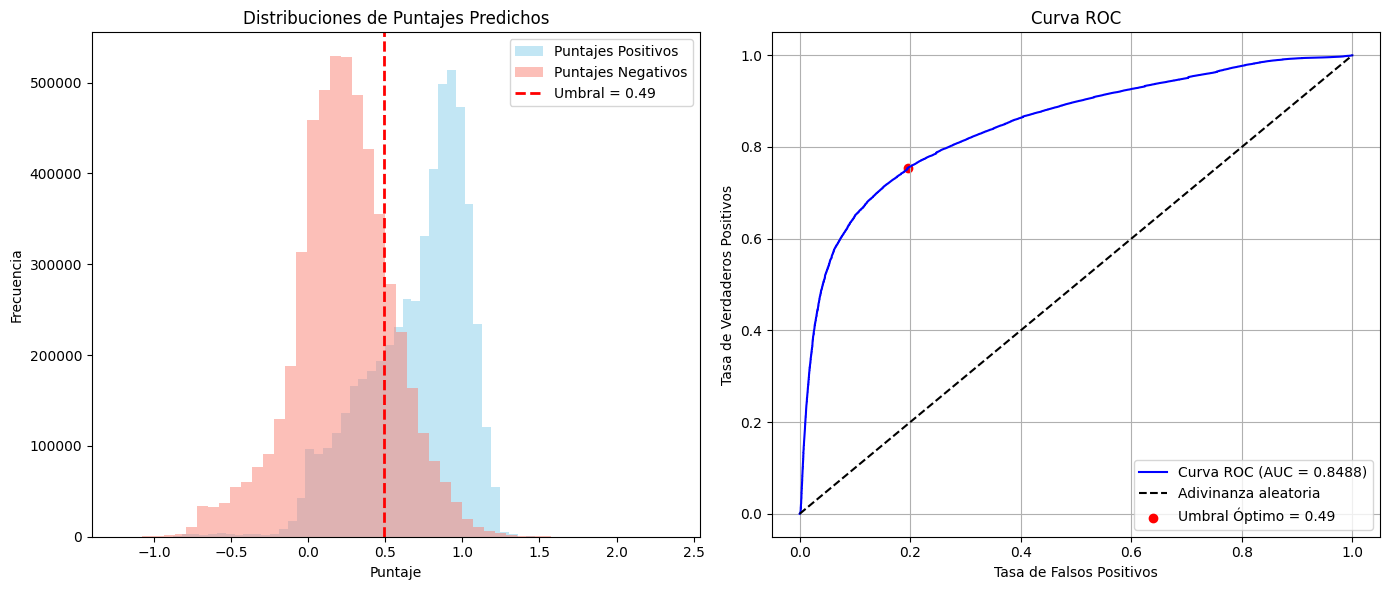
\includegraphics[width=\textwidth]{img/resultados/gnn/partes/caso1_degree/full/roc_GAT_DP_full.png}
        \caption{GAT + Dot Product}
        \label{fig:roc_gat_dp_full}
    \end{subfigure}
    \hfill
    \begin{subfigure}[b]{0.45\textwidth}
        \centering
        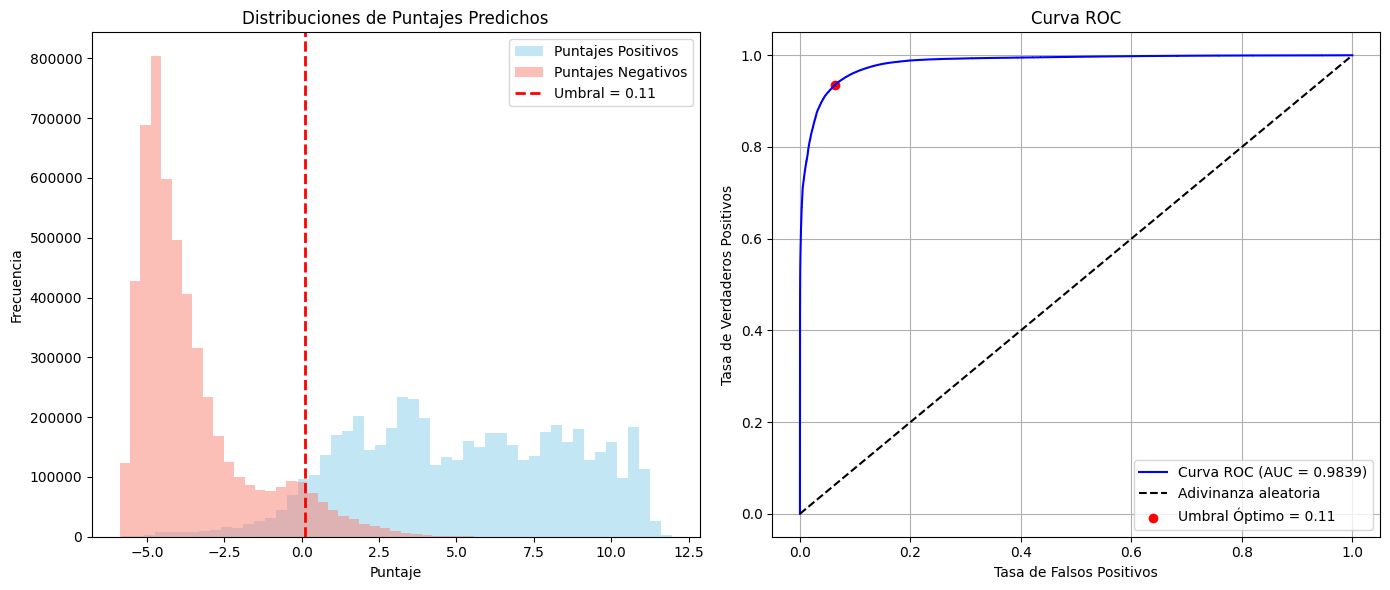
\includegraphics[width=\textwidth]{img/resultados/gnn/partes/caso1_degree/full/roc_GAT_MLP_full.png}
        \caption{GAT + MLP}
        \label{fig:roc_gat_mlp_full}
    \end{subfigure}

    \caption{Curvas ROC y valores AUC para el grafo construido a partir de todas las \texttt{AS\_PATHs}.}
    \label{fig:comparacion_roc_auc_caso1_full}
\end{figure}





\begin{table}[t]
\centering
\begin{tabular}{lccc}
\hline
\textbf{Modelo} & \textbf{Decodificador} & \textbf{AUC}& \textbf{Accuracy(\%)} \\
\hline
GCN & Dot Product & 0.982 & 0.947 \\
GraphSAGE & Dot Product & 0.958 & 0.888 \\
GAT & Dot Product & 0.848 &  0.779 \\
GCN & MLP & 0.990 &  0.948 \\
\textbf{GraphSAGE} & \textbf{MLP} &  \textbf{0.991} & \textbf{0.954} \\
GAT & MLP &  0.983 &  0.936 \\
\hline
\end{tabular}
\caption{Accuracy estimada por combinación de codificador y decodificador.}
\label{tab:accuracy_gnn_full}
\end{table}

\newpage
Podemos observar que el uso de un decoder MLP mejora la capacidad de discriminación entre enlaces positivos y negativos. Se puede ver que en los gráficos donde se usan MLP hay una clara separación entre las clases. 
GraphSAGE con MLP destaca con la mejor combinación (AUC = 0.991, accuracy ≈ 95\%).\\


Luego de la generación de \textit{embeddings}, se evaluó la tarea principal de inferencia de relaciones entre ASes, usando los \textit{embeddings} creados con la tarea previa. En la Tabla~\ref{tab:gnn_resultados_caso1} se muestran los resultados de Precision, Recall y Accuracy obtenidos para cada combinación.\\


\begin{table}[H]
\centering
\resizebox{\textwidth}{!}{
\begin{tabular}{llcccccccccccc}
\toprule
\multirow{2}{*}{\textbf{Modelo}} & 
\multirow{2}{*}{\textbf{Decodificador}} & 
\multicolumn{3}{c}{\textbf{NoBatch-NoW}} & 
\multicolumn{3}{c}{\textbf{NoBatch-W}} & 
\multicolumn{3}{c}{\textbf{Batch-NoW}} & 
\multicolumn{3}{c}{\textbf{Batch-W}} \\
\cmidrule(lr){3-5} \cmidrule(lr){6-8} \cmidrule(lr){9-11} \cmidrule(lr){12-14}
 & & \textbf{Precision} & \textbf{Recall} & \textbf{Accuracy} 
   & \textbf{Precision} & \textbf{Recall} & \textbf{Accuracy} 
   & \textbf{Precision} & \textbf{Recall} & \textbf{Accuracy} 
   & \textbf{Precision} & \textbf{Recall} & \textbf{Accuracy} \\
\midrule
GCN       & Dot Product &74.97&70.91&73.36&71.10&36.84&62.17&74.69&70.72&73.16&63.54&30.52&55.41\\
GraphSAGE & Dot Product &82.99&77.18&80.32&77.56&63.90&72.30&\textbf{82.96}&\textbf{78.88}&\textbf{81.09}&78.71&71.31&75.59\\
GAT       & Dot Product &74.75&70.78&73.15&75.14&39.91&65.74&75.35&71.95&73.99&71.96&49.27&64.41\\
\midrule
GCN       & MLP         &70.06&68.19&69.24&68.80&18.33&48.05&73.17&67.36&71.02&63.76&33.69&55.60\\
GraphSAGE & MLP         &78.92&74.04&76.81&75.94&55.16&69.10&79.70&74.46&77.48&73.01&53.97&66.47\\
GAT       & MLP         &73.93&70.40&72.71&74.33&28.63&62.86&76.42&72.03&74.49&71.43&33.28&59.94\\
\bottomrule
\end{tabular}
}
\caption{Resultados de Precision, Recall y Accuracy (\%) por combinación de encoder y decoder bajo cuatro configuraciones: sin batching y sin balanceo (`NoBatch-NoW'), sin batching con balanceo (`NoBatch-W'), con batching sin balanceo (`Batch-NoW'), y con ambas (`Batch-W'). En negrita se indican los mejores resultados por métrica en cada configuración.}
\label{tab:gnn_resultados_caso1}
\end{table}


Con esto podemos ver que utilizar los atributos provenientes de peeringDB permite obtener mejores resultados que al usar únicamente atributos estructurales básicos como el grado. Asimismo, este caso repite la misma lógica en los resultados donde la MLP es más adecuada como decoder para la tarea auxiliar de link prediction, mientras que Dot Product produce \textit{embeddings} más simples fáciles de analizar para la ANN, lo que resulta en un mejor desempeño en la clasificación final de relaciones entre los Sistemas Autónomos.\\






\subsubsection{Caso 2: Predicción de enlaces utilizando grafo con atributos provenientes de estudios previos}

\begin{itemize}
    \item \textbf{RIBs:} Febrero 2024.
    \item \textbf{Atributos de nodos:} Definidos en un \textit{dataset} utilizado en trabajos anteriores~\cite{BenchmarkingGNN}.
    \item \textbf{Tarea para la creación de \textit{embeddings}:} Determinar la existencia o no de un enlace entre pares de nodos (Sistemas Autónomos).
    \item \textbf{Tamaño \textit{embeddings}:} 32.
    \item \textbf{Epochs:} 100 (GNN) y 20 (ANN).
    \item \textbf{Early Stopping:} Paciencia de 8 epochs.
    \item \textbf{Learning Rate:} 0.001 (GNN) y 0,005 (ANN).
\end{itemize}


Con el objetivo de validar la utilidad de los atributos de nodo definidos en este trabajo, se realizó la inferencia utilizando los atributos propuestos por Giakatos et al.~\cite{BenchmarkingGNN}. Estos atributos fueron extraídos de diferentes fuentes~\cite{PeeringDB,CAIDAAS-rank,BGP2VecCode} y corresponden a la fecha de julio de 2022.  \\

Este grafo, a diferencia del construido en nuestro trabajo, es más pequeño. Esto se debe a que en el estudio de Giakatos et al. se decidió eliminar en tres iteraciones los nodos hoja, es decir, aquellos nodos con grado 1. \\


A continuación, los resultados obtenidos a partir de la tarea para crear \textit{embeddings}. La Tabla~\ref{tab:comparacion_accuracy_caso2_t} resume los valores de AUC y Accuracy alcanzados por cada combinación de encoder y decoder, mientras que la Figura \ref{fig:roc_auc_prev_2022} presenta las curvas ROC asociadas, lo que permite contrastar visualmente el desempeño de cada variante.\\




\begin{figure}[t]
    \centering
    % Primera fila
    \begin{subfigure}[b]{0.45\textwidth}
        \centering
        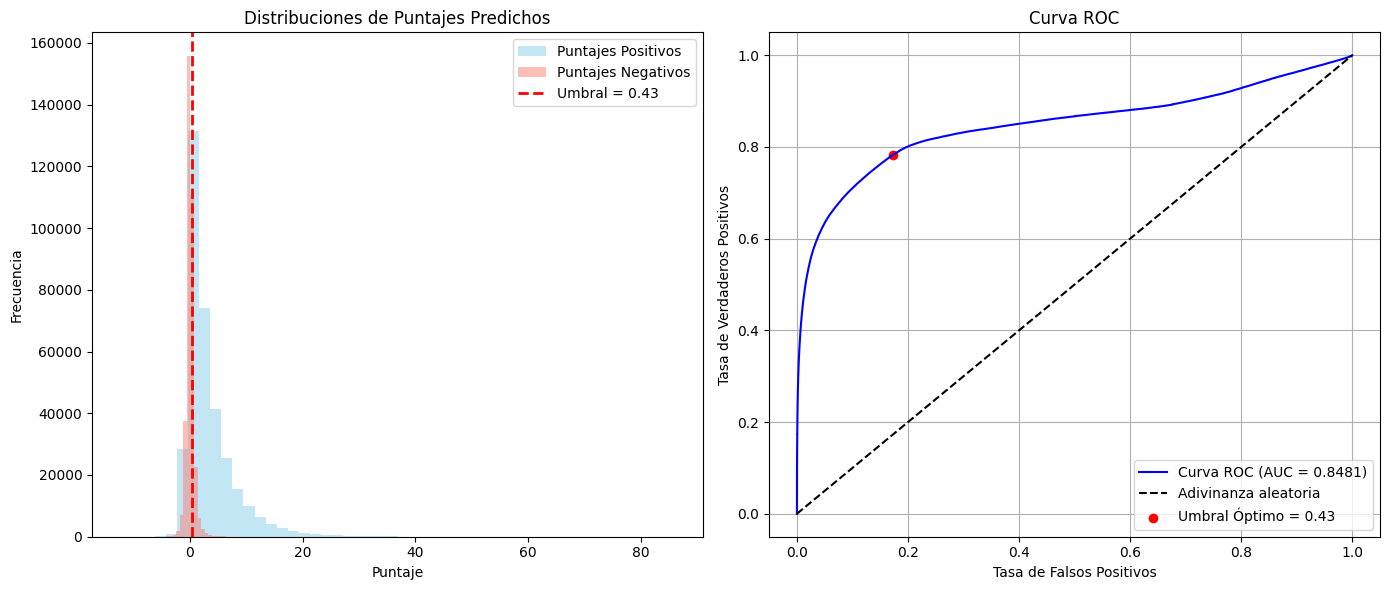
\includegraphics[width=\textwidth]{img//resultados//gnn//partes//caso3_previo/GCN_previo_linkPred.png}
        \caption{GCN + Producto Punto}
    \end{subfigure}
    \hfill
    \begin{subfigure}[b]{0.45\textwidth}
        \centering
        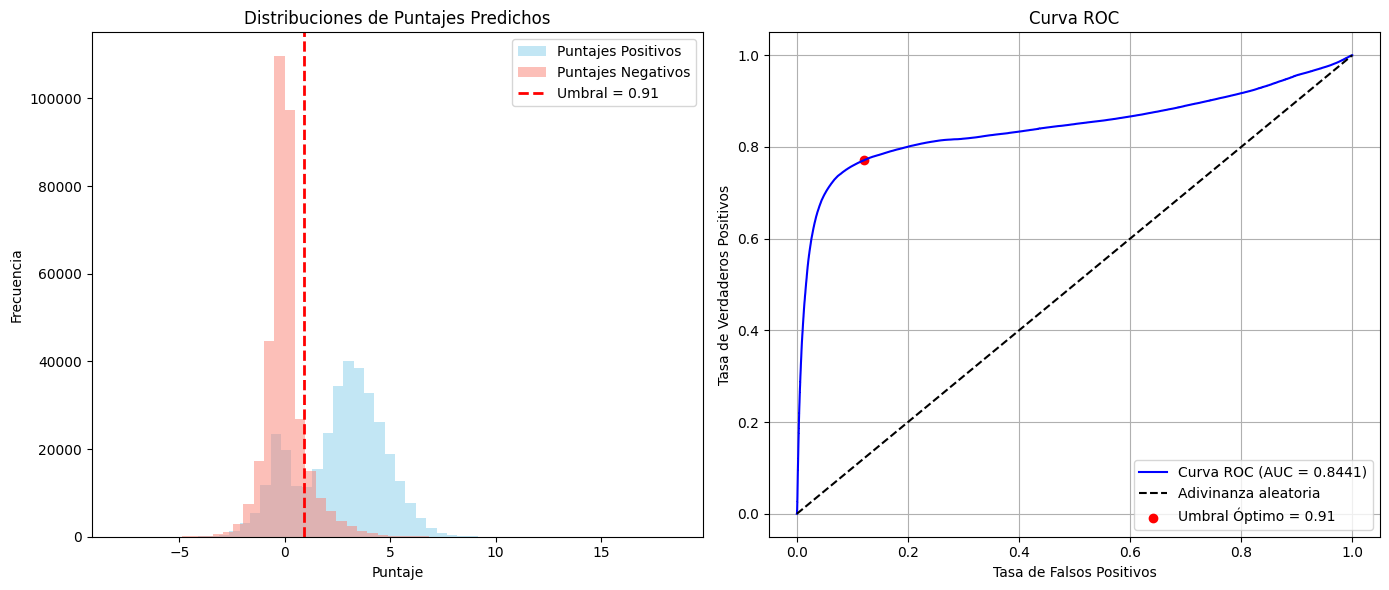
\includegraphics[width=\textwidth]{img//resultados//gnn//partes//caso3_previo/GraphSAGE_previo_LP.png}
        \caption{GraphSAGE + Producto Punto}
        \label{fig:conf_matrix_sage_dp_prev}
    \end{subfigure}

    \vspace{0.5cm}

    % Segunda fila
    \begin{subfigure}[b]{0.45\textwidth}
        \centering
        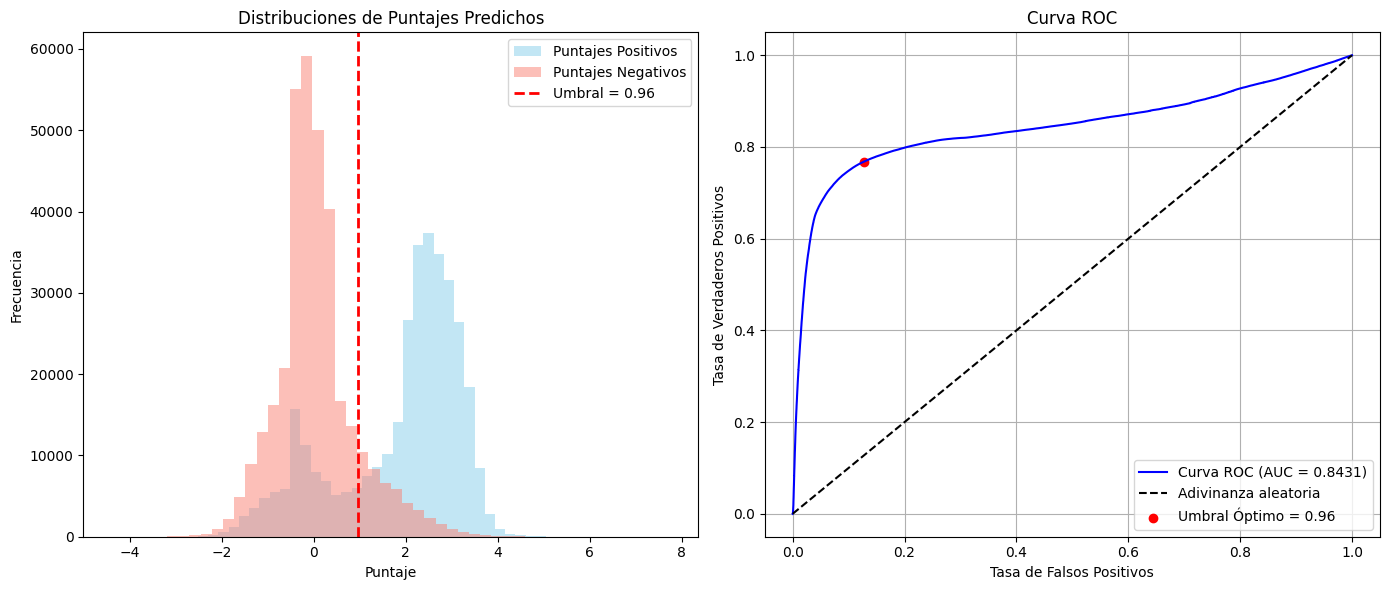
\includegraphics[width=\textwidth]{img//resultados//gnn//partes//caso3_previo/GAT_previo_LP.png}
        \caption{GAT + Producto Punto}
    \end{subfigure}
    \hfill
    \begin{subfigure}[b]{0.45\textwidth}
        \centering
        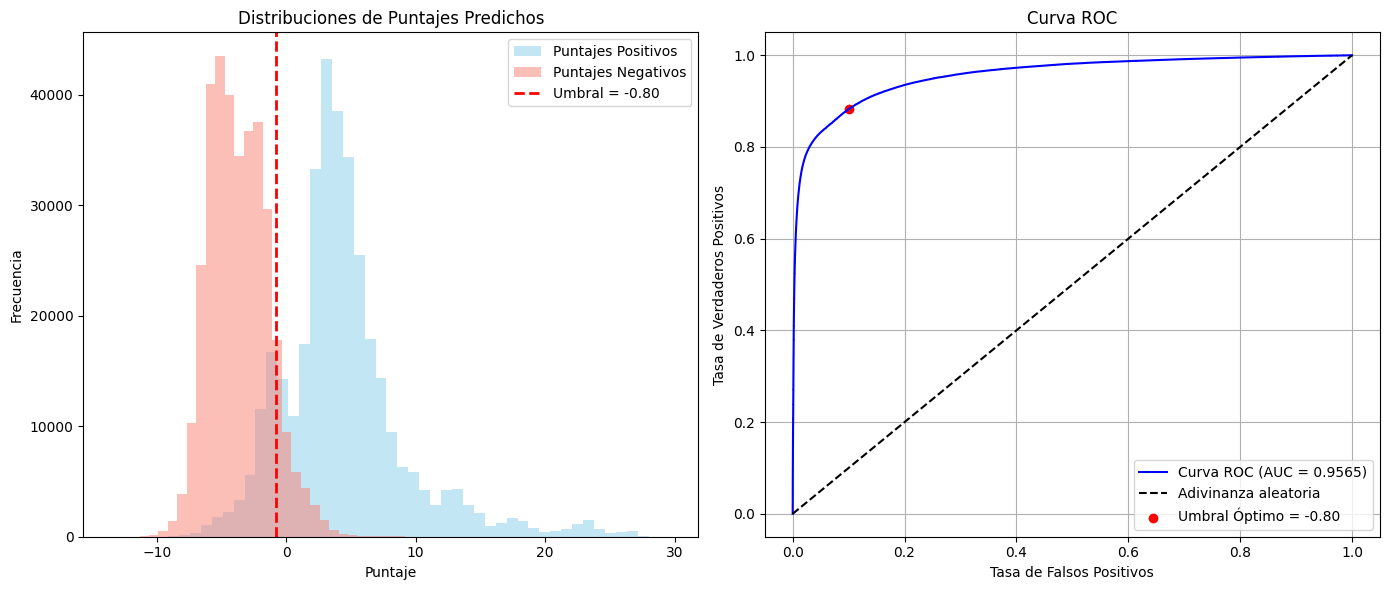
\includegraphics[width=\textwidth]{img//resultados//gnn//partes//caso3_previo/GCN_MLP_previo_LP.png}
        \caption{\textbf{GCN + MLP}}
    \end{subfigure}

    \vspace{0.5cm}

    % Tercera fila
    \begin{subfigure}[b]{0.45\textwidth}
        \centering
        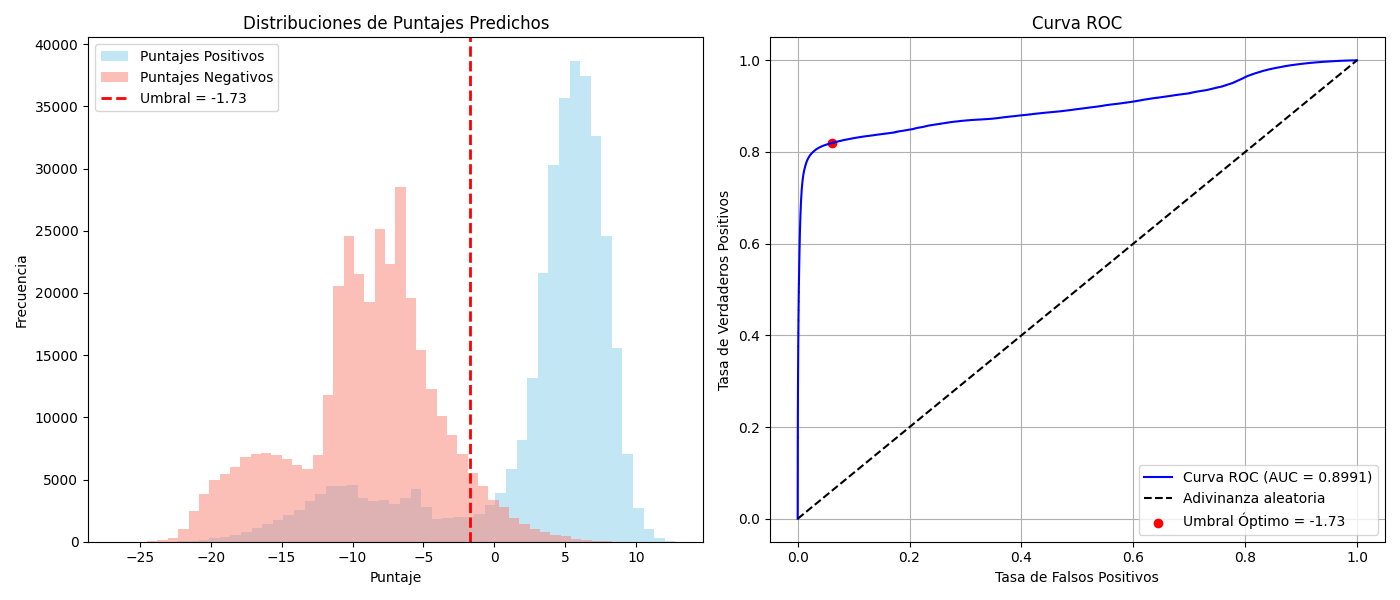
\includegraphics[width=\textwidth]{img/resultados/gnn/partes/caso3_previo/roc_curve_GraphSAGE_MLP.png}
        \caption{GraphSAGE + MLP}
    \end{subfigure}
    \hfill
    \begin{subfigure}[b]{0.45\textwidth}
        \centering
        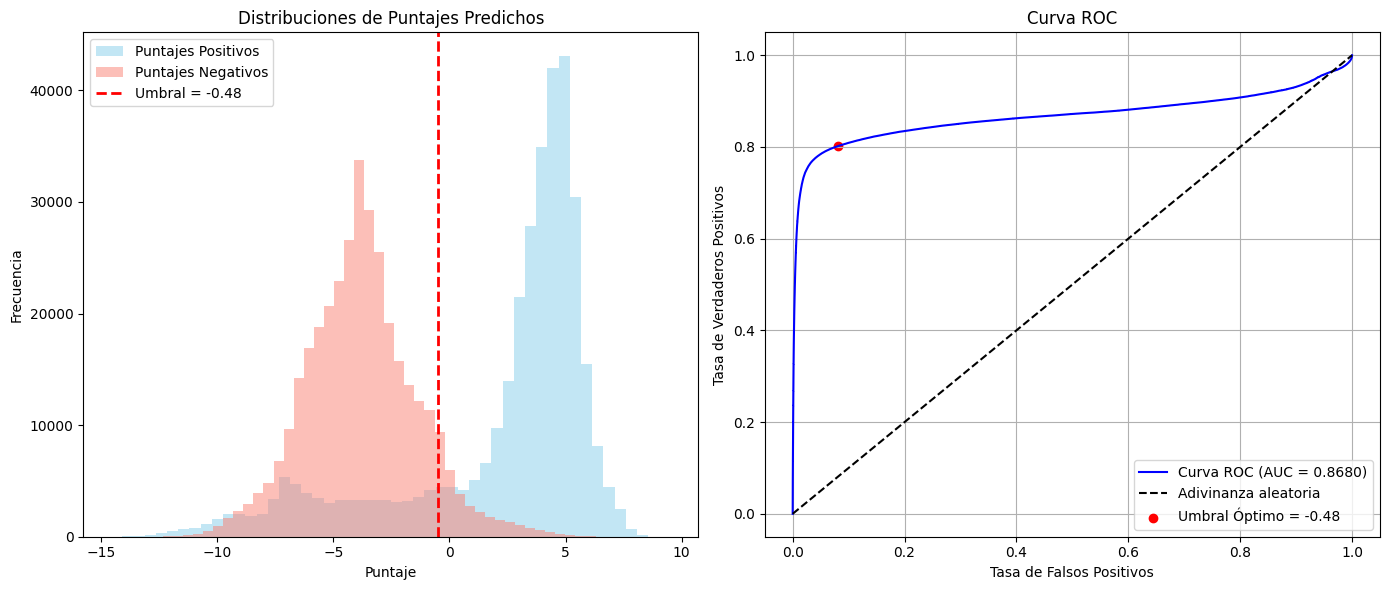
\includegraphics[width=\textwidth]{img//resultados//gnn//partes//caso3_previo/GAT_MLP_previo_LP.png}
        \caption{GAT + MLP}
    \end{subfigure}

    \caption{Curvas ROC y distribución de los resultados. Con diferentes encoders y decoders para grafo con atributos de julio 2022.}
    \label{fig:roc_auc_prev_2022}
\end{figure}



\begin{table}[H]
\centering
\begin{tabular}{lccc}
\hline
\textbf{Modelo} & \textbf{Decodificador} & \textbf{AUC}& \textbf{Accuracy (\%)} \\
\hline
GCN & Dot Product & 0.848  & 0.805 \\
GraphSAGE & Dot Product & 0.844 & 0.825 \\
GAT & Dot Product & 0.843 & 0.820 \\
\textbf{GCN} & \textbf{MLP} & \textbf{0.956} &  \textbf{0.891} \\
GraphSAGE & MLP &  0.937 & 0.874 \\
GAT & MLP & 0.860 & 0.857 \\
\hline
\end{tabular}
\caption{Accuracy de la inferencia con link prediction para la creación de \textit{embeddings}.}
\label{tab:comparacion_accuracy_caso2_t}
\end{table}



Luego de la generación de \textit{embeddings}, se evaluó la tarea principal. En la Tabla~\ref{tab:comparacion_metricas_caso2_now_w} se muestran los resultados obtenidos para cada combinación.\\


\begin{table}[H]
\centering
\resizebox{0.9\textwidth}{!}{
\begin{tabular}{llcccccc}
\toprule
\multirow{2}{*}{\textbf{Modelo}} & 
\multirow{2}{*}{\textbf{Decodificador}} & 
\multicolumn{3}{c}{\textbf{NoBatch-NoW}} & 
\multicolumn{3}{c}{\textbf{NoBatch-W}} \\
\cmidrule(lr){3-5} \cmidrule(lr){6-8}
 & & \textbf{Precision} & \textbf{Recall} & \textbf{Accuracy} 
   & \textbf{Precision} & \textbf{Recall} & \textbf{Accuracy} \\
\midrule
GCN       & Dot Product &82.47&77.02&80.03&80.07&69.73&75.95\\
          & MLP         &79.25&74.73&77.15&73.03&56.64&67.39\\
\midrule
GraphSAGE & Dot Product &\textbf{85.14}&\textbf{82.18}&\textbf{83.76}&79.97&69.27&75.81\\
          & MLP         &75.63&72.60&74.21&68.44&43.77&62.66\\
\midrule
GAT       & Dot Product &84.56&79.89&82.35&78.04&68.46&74.31\\
          & MLP         &77.31&71.85&75.06&65.10&44.02&59.31\\
\bottomrule
\end{tabular}
}
\caption{Resultados de Precision, Recall y Accuracy (\%) por combinación de encoder y decoder bajo dos configuraciones: sin batching y sin balanceo (`NoBatch-NoW'), y sin batching con balanceo (`NoBatch-W'). En negrita se indican los mejores resultados por métrica.}
\label{tab:comparacion_metricas_caso2_now_w}
\end{table}


Para la tarea principal de clasificación de relaciones (C2P, P2P, P2C) se repiten los resultados observados en los Casos 0 y 1: los \textit{embeddings} generados con Dot Product superan en desempeño a los obtenidos con MLP, siendo GraphSAGE + Dot Product la mejor combinación, con una Accuracy ≈ 83.8\% y un Recall ≈ 82.2\%. 
En cuanto al uso de pesos para balancear las clases (P2P mayoritaria), las métricas se reducen de manera significativa. Este experimento genera resultados ligeramente inferiores a los del Caso 0 (Recall ≈ 83\% y Accuracy ≈ 85\%), lo que refuerza la idea de que los atributos diseñados en este trabajo aportan información para distintas tareas en el ámbito de Internet. Esto es porque los atributos del estudio de Giakatos et al.~\cite{BenchmarkingGNN} fueron creados como una base para analizar diferentes tareas exploratorias usando GNNs.\\


%- Con lr 0.05 y sin class wight todas (los 6 casos) predicen p2p
%- Los q ocupan MLP sin class wieght obtienen malos resulatados, tind a predecir como p2p a los p2c y c2p






\subsubsection{Caso 3: Predicción del grado de los nodos utilizando grafo con atributos extraídos de PeeringDB}

\begin{itemize}
    \item \textbf{RIBs:} Febrero 2024.
    \item \textbf{Atributos de nodos:} Dataset creado a partir de PeeringDB.
    \item \textbf{Epochs:} 20.
    \item \textbf{Tarea para la creación de \textit{embeddings}:} Determinar el grado de salida (out-degree) de cada nodo.
    \item \textbf{Tamaño \textit{embeddings}:} 32.
    \item \textbf{Epochs:} 100 (GNN) y 20 (ANN).
    \item \textbf{Early Stopping:} Paciencia de 8 epochs.
    \item \textbf{Learning Rate:} 0.001 (GNN) y 0,001 (ANN).
\end{itemize}

Para este caso, se utilizó la tarea de inferencia del grado de los nodos para la creación de los \textit{embeddings}. Se seleccionó este atributo (grado de salida) debido a que muchas métricas (por ejemplo, el PageRank clásico) se basan principalmente en el grado de salida, ya que representa la cantidad de conexiones que un nodo ofrece hacia otros.\\


%\newpage
%Luego tenemos prediccion del atributo grado, se ocupa el grado de salida porque primero muchos métodos (por ejemplo, PageRank clásico) se basan principalmente en el out-degree, ya que la idea es repartir "importancia" hacia afuera. En nuestro caso el out-degree suele reflejar cuántas conexiones directas ofrece un nodo hacia otros. Por otro lado vimos en lso resultados que generalmente son los mismos nodos que tienne mayor cantidad de in y out degree.\\


Antes del entrenamiento, el grado de los nodos fue calculado y posteriormente se le aplicó una transformación logarítmica, esto porque, como se observó en la Figura~\ref{fig:distribucion_as_grado_salida_entrada_febrero_log}, la distribución del grado de los nodos presenta una alta concentración, donde pocos Sistemas Autónomos poseen un gran número de conexiones y la mayoría tiene pocos. Finalmente, se realizó una normalización para ajustar los valores resultantes al intervalo $[0,1]$, facilitando así el proceso de entrenamiento.\\



\begin{figure}[H]
    \centering
    \begin{subfigure}[b]{0.4\linewidth}
        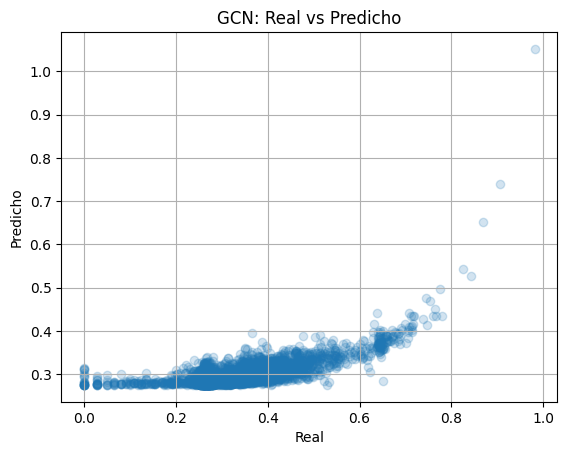
\includegraphics[width=\linewidth]{img//resultados//gnn//partes//caso4_attr_pred//degree/distr_gcn_1m.png}
        \caption{\textbf{GCN}}
        \label{fig:gcn_real_pred}
    \end{subfigure}
    \hfill
    \begin{subfigure}[b]{0.4\linewidth}
        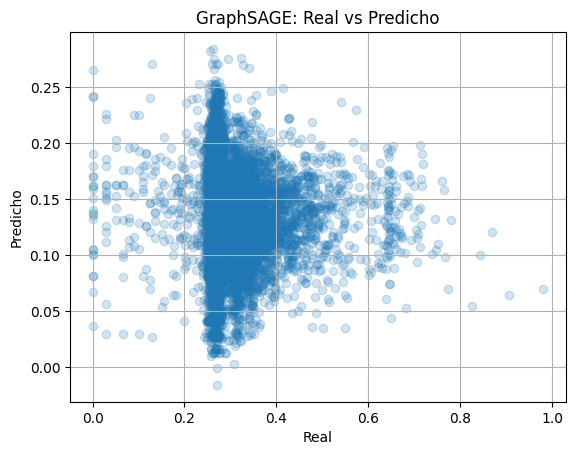
\includegraphics[width=\linewidth]{img//resultados//gnn//partes//caso4_attr_pred//degree/distr_graphsage_1m.png}
        \caption{GraphSAGE}
        \label{fig:graphsage_real_pred}
    \end{subfigure}
    \hfill
    \begin{subfigure}[b]{0.4\linewidth}
        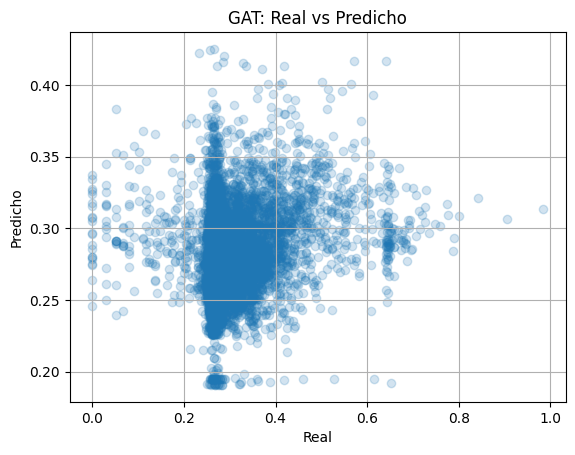
\includegraphics[width=\linewidth]{img//resultados//gnn//partes//caso4_attr_pred//degree/dist_gat_1m.png}
        \caption{GAT}
        \label{fig:gat_real_pred}
    \end{subfigure}
    
    \caption{Comparación entre valores reales y predichos por los modelos GCN, GraphSAGE y GAT.}
    \label{fig:comparacion_real_vs_pred}
\end{figure}

%En la Figura~\ref{fig:comparacion_real_vs_pred} se presenta una comparación entre los valores reales y los predichos por los modelos GCN, GraphSAGE y GAT.\\


La Figura~\ref{fig:gcn_real_pred} muestra los resultados del modelo GCN, donde se observa una tendencia general, aunque el modelo tiende a subestimar los valores. Por otro lado, las Figuras~\ref{fig:graphsage_real_pred} y \ref{fig:gat_real_pred} presentan predicciones concentradas en torno a un valor promedio. Se probaron varios ajustes para intentar solucionar esto, incluyendo cambios en la tasa de aprendizaje, usar una función de pérdida diferente  y aumentar la cantidad de epochs; sin embargo, ninguno de estos ajustes logró una mejora en los resultados. Sugiriendo que GraphSAGE y GAT tienen dificultad para capturar la variabilidad real del grado de salida, es decir, una baja capacidad de generalización.\\



La Tabla~\ref{tab:resultados_regresion_outdegree} muestra las métricas que reflejan el desempeño de cada modelo.\\

\begin{table}[H]
\centering
\caption{Desempeño de arquitecturas GNN para la predicción del atributo \textit{out\_degree} transformado con logaritmo.}
\label{tab:resultados_regresion_outdegree}
\begin{tabular}{lccc}
\toprule
\textbf{Modelo} & \textbf{MAE} & \textbf{MSE} & \textbf{$R^2$} \\
\midrule
GCN        & \textbf{0.0437}  & \textbf{0.00297}  & \textbf{0.1793} \\
GraphSAGE  & 0.0803  & 0.00597  & -1.111 \\
GAT        & 0.0486  & 0.04862  & -0.055  \\
\bottomrule
\end{tabular}
\end{table}



Luego de la generación de \textit{embeddings}, se evaluó la tarea principal. La Tabla~\ref{tab:accuracy_outdegree_downstream} resume los resultados de Precision, Recall y Accuracy.

\begin{table}[H]
\centering
\resizebox{0.7\textwidth}{!}{
\begin{tabular}{lcccccc}
\toprule
\multirow{2}{*}{\textbf{Modelo}} &
\multicolumn{3}{c}{\textbf{NoBatch-NoW}} &
\multicolumn{3}{c}{\textbf{NoBatch-W}} \\
\cmidrule(lr){2-4} \cmidrule(lr){5-7}
 & \textbf{Precision} & \textbf{Recall} & \textbf{Accuracy} 
 & \textbf{Precision} & \textbf{Recall} & \textbf{Accuracy} \\
\midrule
GCN       &67.40&65.52&67.24&62.52&1.39&45.27\\
GraphSAGE &\textbf{84.61}&\textbf{79.65}&\textbf{82.29}& 79.54 & 71.24 & 75.80 \\
GAT       &84.55&76.09&80.70& 78.63 & 67.51 & 73.89 \\
\bottomrule
\end{tabular}
}
\caption{Resultados de Precision, Recall y Accuracy (\%) por modelo GNN bajo dos configuraciones: sin balanceo de clases (`NoBatch-NoW') y con balanceo de clases (`NoBatch-W').}
\label{tab:accuracy_outdegree_downstream}
\end{table}


Con estos resultados podemos ver el impacto de la tarea auxiliar sobre la creación de las representaciones vectoriales de los nodos. Para este caso, si bien GCN obtuvo los mejores resultados en la tarea auxiliar de predicción de grado de salida, sus \textit{embeddings} resultan poco útiles para la clasificación de relaciones entre ASes, 
es decir, no capturan propiedades relevantes para diferenciar relaciones económicas. En cambio, GraphSAGE y GAT, aunque fallan en predecir bien el grado, producen \textit{embeddings} más ricos para la tarea final.\\ 



\subsubsection{Caso 4: Predicción del valor de PageRank utilizando grafo con atributos extraídos de PeeringDB.}

\begin{itemize}
    \item \textbf{RIBs:} Febrero 2024.
    \item \textbf{Atributos de nodos:} Dataset creado a partir de PeeringDB.
    \item \textbf{Epochs:} 100 (GNN) y 20 (ANN).
    \item \textbf{Tarea para la creación de \textit{embeddings}:} Predicción del valor de PageRank de cada nodo, una métrica de centralidad que refleja su importancia en el grafo.
    \item \textbf{Early Stopping:} Paciencia de 8 epochs.
    \item \textbf{Learning Rate:} 0.001 (GNN) y 0,001 (ANN).
\end{itemize}



Primero, se calculó el valor de PageRank para cada nodo, como estos valores tienden a concentrarse en rangos pequeños con algunos valores extremos, se aplicó una transformación logarítmica, con el objetivo de reducir la dispersión y estabilizar la escala. Luego, se normalizó el resultado utilizando una transformación tipo \textit{z-score}.\\







\begin{figure}[H]
    \centering
    % ---------- Fila 1 ----------
    \begin{subfigure}[b]{0.40\linewidth}
        \centering
        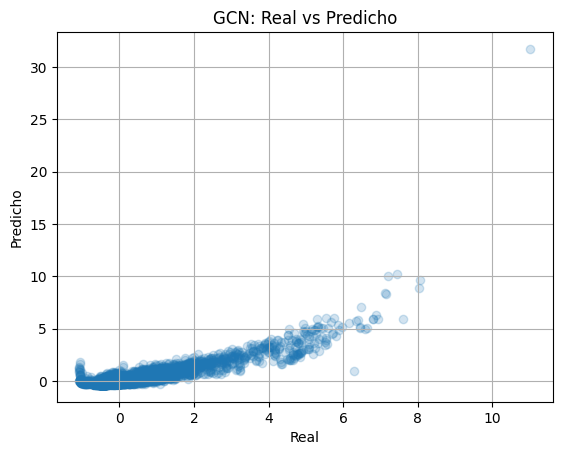
\includegraphics[width=\linewidth]{img//resultados//gnn//partes//caso5/distr_gcn.png}
        \caption{GCN}
        \label{fig:distr_gcn}
    \end{subfigure}
    \hfill
    \begin{subfigure}[b]{0.40\linewidth}
        \centering
        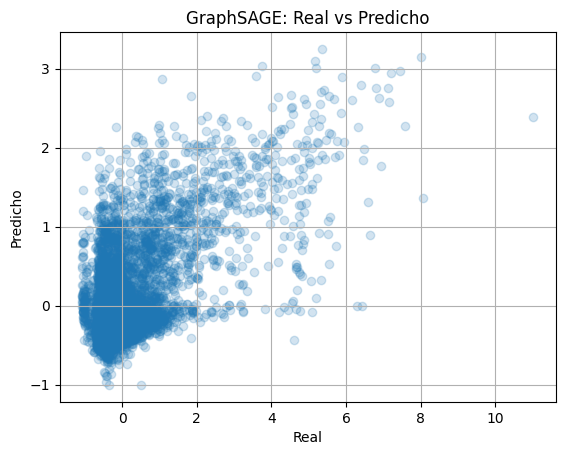
\includegraphics[width=\linewidth]{img//resultados//gnn//partes//caso5/distr_graphsage.png}
        \caption{GraphSAGE}
        \label{fig:distr_graphsage}
    \end{subfigure}

    \vspace{0.8em} % separación vertical entre filas

    % ---------- Fila 2 ----------
    \begin{subfigure}[b]{0.40\linewidth}
        \centering
        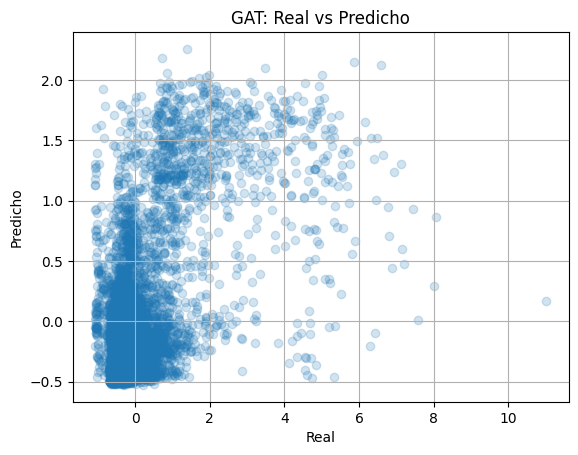
\includegraphics[width=\linewidth]{img//resultados//gnn//partes//caso5/distr_gat.png}
        \caption{GAT}
        \label{fig:distr_gat}
    \end{subfigure}

    \caption{Comparación entre valores reales y predichos por los modelos
GCN, GraphSAGE y GAT.}
    \label{fig:distr_gnn_all}
\end{figure}

La Tabla~\ref{tab:resultados_test_modelos_pagerank} muestra los resultados obtenidos en el conjunto de test para cada arquitectura utilizada.

\begin{table}[H]
\centering
\begin{tabular}{lccc}
\toprule
\textbf{Modelo} & \textbf{MSE} & \textbf{MAE} & \textbf{$R^2$} \\
\midrule
GCN       & \textbf{0.242087} & \textbf{0.316427} & \textbf{0.746798} \\
GraphSAGE & 0.560129 & 0.439433 & 0.414153 \\
GAT       & 0.639733 & 0.463012 & 0.330895 \\
\bottomrule
\end{tabular}
\caption{Resultados para la tarea de predicción de PageRank utilizando distintas arquitecturas GNN. En negrita se resaltan los mejores resultados por métrica.}
\label{tab:resultados_test_modelos_pagerank}
\end{table}



Al igual que en el caso anterior, podemos ver que GCN (Figura~\ref{fig:distr_gcn}) es la que sigue mejor la diagonal, aunque empieza a subestimar los nodos con PageRank más alto. Por otro lado, GraphSAGE y GAT (Figuras~\ref{fig:distr_graphsage} y \ref{fig:distr_gat}) concentran muchos puntos cerca de un valor promedio, lo que indica que les cuesta distinguir los extremos, pero aun así capturan suficiente estructura para la tarea siguiente de inferencia.\\

En cuanto a la tarea \textit{downstream}, la Tabla~\ref{tab:downstream_caso4} muestra los resultados obtenidos en la tarea de inferencia de relaciones a partir de los \textit{embeddings} generados durante la predicción de PageRank. Se presentan los valores de Accuracy tanto para el caso con y sin balance de clases.\\




\begin{table}[H]
\centering
\resizebox{0.7\textwidth}{!}{
\begin{tabular}{lcccccc}
\toprule
\multirow{2}{*}{\textbf{Modelo}} &
\multicolumn{3}{c}{\textbf{NoBatch-NoW}} &
\multicolumn{3}{c}{\textbf{NoBatch-W}} \\
\cmidrule(lr){2-4} \cmidrule(lr){5-7}
 & \textbf{Precision} & \textbf{Recall} & \textbf{Accuracy} 
 & \textbf{Precision} & \textbf{Recall} & \textbf{Accuracy} \\
\midrule
GCN       & 78.55 & 73.04 & 76.29 & 72.16 & 48.21 & 63.30 \\
GraphSAGE & \textbf{86.74} & \textbf{83.58} & \textbf{85.17} & 80.20 & 73.97 & 77.445 \\
GAT       & 84.46 & 79.08 & 81.98 & 80.31 & 71.68 & 76.64 \\
\bottomrule
\end{tabular}
}
\caption{Resultados de Precision, Recall y Accuracy (\%) por modelo GNN bajo dos configuraciones: sin balanceo de clases (`NoBatch-NoW') y con balanceo de clases (`NoBatch-W').}
\label{tab:downstream_caso4}
\end{table}



Aquí se observa que la predicción de PageRank como tarea auxiliar para la creación de embeddings es más apropiada que la predicción de grado para generar \textit{embeddings} de Sistemas Autónomos, donde GCN obtiene el mejor desempeño ($R^2$ ≈ 0.75), mientras que GraphSAGE y GAT muestran un mayor nivel de dispersión y menor poder explicativo. Sin embargo, todos los modelos tienen dificultad  para representar valores extremos, lo que muestra una limitación al trabajar con distribuciones muy desiguales (\textit{long tail}), típicas de la topología de Internet.\\



En comparación con los casos anteriores, este caso, al predecir PageRank, permite generar \textit{embeddings} más informativos que los obtenidos al predecir el grado (Caso 3), capturando mejor la centralidad y relevancia global de los nodos. Sin embargo, los resultados finales son inferiores a los alcanzados por la tarea  de predicción de enlaces (Casos 0, 1 y 2), lo que nos dice que esa tarea es más efectiva para este problema.\\

\newpage
\subsubsection{Caso 5: Creación de \textit{embeddings} a partir de DeepWalk y BGP2Vec}

\begin{itemize}
    \item \textbf{RIBs:} Febrero 2024.
    \item Se aplicó el algoritmo DeepWalk y BGP2Vec para generar una representación vectorial (\textit{embedding}) para cada nodo, basada en recorridos aleatorios.
    \item \textbf{Tarea para la creación de \textit{embeddings}:}
    \item \textbf{Epochs:} 100 (GNN) y 20 (ANN).
    \item \textbf{Early Stopping:} Paciencia de 8 epochs (ANN).
    \item \textbf{Learning Rate:} 0,001 (ANN).
\end{itemize}

La Tabla~\ref{tab:accuracy_gnn_variants_dw_bgp2vc} muestra los resultados obtenidos para la tarea de inferencia a partir de la creación de \textit{embeddings} con los métodos de DeepWalk y BGP2Vec .\\



\begin{figure}[H]
    \centering
    \begin{subfigure}[t]{0.48\textwidth}
        \centering
        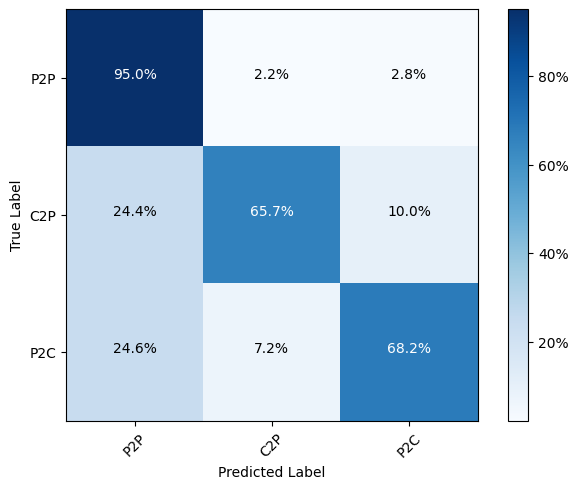
\includegraphics[width=\linewidth]{img//resultados//gnn//partes//caso5/mc_deepwalk_nobatch_noweight.png}
        \caption{DeepWalk}
        \label{fig:mc_deepwalk}
    \end{subfigure}%
    \hfill
    \begin{subfigure}[t]{0.48\textwidth}
        \centering
        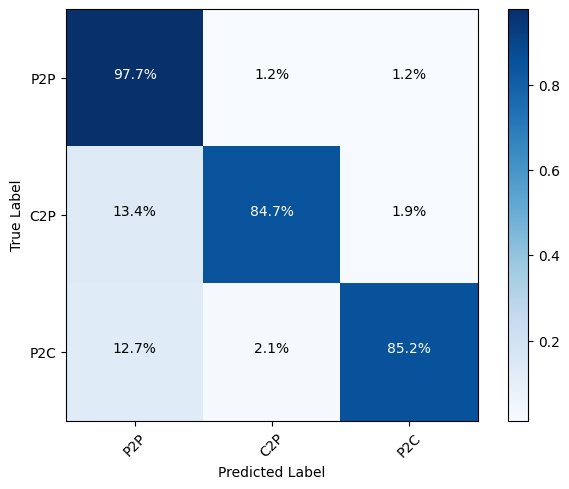
\includegraphics[width=\linewidth]{img//resultados//gnn//partes//caso5/mc_bgp2vec.png}
        \caption{BGP2Vec}
        \label{fig:mc_bgp2vec}
    \end{subfigure}
    \caption{Matrices de confusión obtenidas a partir de los resultados de inferencia utilizando \textit{embeddings} generados con DeepWalk y BGP2Vec.}
    \label{fig:mc_comparacion}
\end{figure}




\begin{table}[H]
\centering
\resizebox{\textwidth}{!}{
\begin{tabular}{lcccccccccccc}
\toprule
\multirow{2}{*}{\textbf{Modelo}} & 
\multicolumn{3}{c}{\textbf{NoBatch-NoW}} & 
\multicolumn{3}{c}{\textbf{NoBatch-W}} & 
\multicolumn{3}{c}{\textbf{Batch-NoW}} & 
\multicolumn{3}{c}{\textbf{Batch-W}} \\
\cmidrule(lr){2-4} \cmidrule(lr){5-7} \cmidrule(lr){8-10} \cmidrule(lr){11-13}
 & \textbf{Precision} & \textbf{Recall} & \textbf{Accuracy} 
 & \textbf{Precision} & \textbf{Recall} & \textbf{Accuracy} 
 & \textbf{Precision} & \textbf{Recall} & \textbf{Accuracy} 
 & \textbf{Precision} & \textbf{Recall} & \textbf{Accuracy} \\
\midrule
DeepWalk  & \textbf{86.99} & \textbf{82.78} & \textbf{84.81} & 84.28 & 81.09 & 82.82 & 87.54 & 85.43 & 86.43 & 84.05 & 81.68 & 82.92 \\
BGP2Vec   & \textbf{94.15} & \textbf{93.72} & \textbf{93.92} & 92.24 & 91.83 & \textbf{92.02} & 94.66 & 94.32 & 94.48 & 92.20 & 91.64 & 91.90 \\
\bottomrule
\end{tabular}
}
\caption{Resultados de Precision, Recall y Accuracy (\%) para la inferencia utilizando \textit{embeddings} generados con DeepWalk y BGP2Vec bajo cuatro configuraciones: sin batching y sin balanceo (`NoBatch-NoW'), sin batching con balanceo (`NoBatch-W'), con batching sin balanceo (`Batch-NoW'), y con ambas (`Batch-W').}
\label{tab:accuracy_gnn_variants_dw_bgp2vc}
\end{table}


%Para estos casos d batching hubo early stoping, en el ccas batch con waight en epochs epoch 9 y en batch sin weigh el 11. =que nos dice eso???

%Poner si os i amtroz bgp 2 vec pues s eve super bacan y si redcococe p2c y c2p , no los pone como p2p2

%Deep walk batchin sin weight tuvo arly stoping en poch 12


%bgp2vec early stoping en 16 con batch y wught



\newpage
Podemos ver que los métodos de generación de \textit{embeddings} basados en recorridos aleatorios, entregan un desempeño superior al de las tareas auxiliares de GNN planteadas en los Casos 0 al 4. DeepWalk alcanza una Accuracy ≈ 85\% (similar a casos anteriores), pero BGP2Vec sobresale con una Accuracy de 92\% y Precision/Recall más equilibrada. Estos resultados sugieren que incorporar información derivada de las rutas BGP permite capturar la estructura y jerarquía de la red, superando a las tareas auxiliares basadas en predicción de enlaces o atributos nodales.\\


%////////////////////////////////////////////////////////////////
\subsection{Resultados de Entrenamiento \textit{End-to-End}} \label{sec:entrenamiento_end_to_end}

En este enfoque, el modelo GNN se entrena directamente para predecir el tipo de relación entre pares de Sistemas Autónomos (ASes), integrando todas las etapas del pipeline en un solo proceso. El flujo de trabajo consistió en los siguientes pasos:
\begin{enumerate}
    \item Importación de los RIBs (Routing Information Base) y construcción del grafo en DGL.
    \item Asociación de atributos a cada nodo del grafo (AS). Se probaron tres tipos de atributos:
    \begin{itemize}
        \item Atributos provistos por el dataset base (extraídos del trabajo de Giakatos et al.~\cite{BenchmarkingGNN}).
        \item Atributos definidos a partir de datos obtenidos de PeeringDB.
        \item Métricas de centralidad computadas directamente desde el grafo (por ejemplo, grado, cercanía, intermediación).
    \end{itemize}
    \item Selección del tipo de GNN y del predictor a utilizar. Como se mencionó en la sección anterior, se exploraron modelos como GraphSAGE y GCN, junto a un MLP como clasificador final.

\end{enumerate}

A diferencia del enfoque anterior, durante el entrenamiento se trabajó con un único grafo, los conjuntos de entrenamiento y test se generan mediante máscaras sobre las aristas, en lugar de crear subgrafos.\\

En cuanto al \textit{split}, ambas aristas dirigidas que conforman un mismo par de AS (src, dst) se asignan al mismo conjunto de datos, de modo que la información de una relación no aparezca simultáneamente en entrenamiento y prueba.\\


A continuación, se presentan los diferentes experimentos creados con este enfoque.\\



\subsubsection{Caso 0: Se utiliza grafo con atributos de nodos extraídos de PeeringDB}

\begin{itemize}
    \item \textbf{RIBs:} Febrero 2024.
    \item \textbf{Atributos de nodos:} Dataset creado a partir de PeeringDB.
    \item \textbf{Epochs:} 100.
    \item \textbf{Early Stopping:} Paciencia de 8 epochs.
    \item \textbf{Learning Rate:} de 0,02.
\end{itemize}

Se entrena el modelo sobre la tarea específica de clasificación de aristas para saber la relación económica que dos Sistemas Autónomos comparten. Este primer caso utiliza los atributos creados a partir de PeeringDB.\\

% El grafo construido utilizado para este enfoque cuenta con un total de 401.308 nodos y 1.676.600 aristas dirigidas. Cada nodo posee un vector de atributos de dimensión 68. En cuanto a las aristas, se asignaron etiquetas económicas según el dataset de CAIDA: un total de 977.554 aristas fueron etiquetadas, mientras que 699.046 no poseen etiqueta.\\


% La distribución de clases fue la siguiente:
% \begin{itemize}
%     \item \texttt{C2P}: 668.732 aristas
%     \item \texttt{P2C}: 154.411 aristas
%     \item \texttt{P2P}: 154.411 aristas
%     \item Sin etiqueta: 699.046 aristas (marcadas como $-1$)
% \end{itemize}



\begin{table}[H]
\centering
\caption{Resultados de clasificación por modelo utilizando decodificadores Bilinear y MLP.}
\label{tab:resultados_caso0_bilinear_mlp_500ep}
\resizebox{\textwidth}{!}{
\begin{tabular}{llccc}
\toprule
\textbf{Modelo} & \textbf{Decoder} & \textbf{Precision (\%)} & \textbf{Recall (\%)} & \textbf{Accuracy (\%)} \\
\midrule
GCN       & Bilinear & 88.26 & 85.90 &  91.01 \\
GraphSAGE & Bilinear & 90.53 & 87.78 & 92.57 \\
GAT       & Bilinear & 85.19 & 86.25 & 90.56 \\
\midrule
GCN       & MLP      & 87.74 & 82.00 & 89.41 \\
GraphSAGE & MLP      & \textbf{91.06} & \textbf{89.85} & \textbf{93.48} \\
GAT       & MLP      & 89.44 & 85.22 & 91.57 \\
\bottomrule
\end{tabular}
}
\end{table} 





Como se muestra en la Tabla~\ref{tab:resultados_caso0_bilinear_mlp_500ep}, GraphSAGE alcanza el mejor desempeño general, con un 93,48\% de \textit{Accuracy} al igual que en Precision y Recall.\\

\begin{figure}[H]
    \centering

    \begin{minipage}[b]{0.32\linewidth}
        \centering
        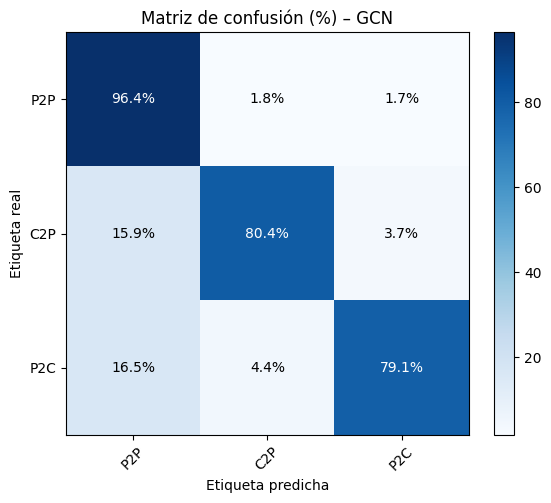
\includegraphics[width=\linewidth]{img//resultados//gnn//end-to-end//caso0/mc_gcn_caso0_b.png}
%        \caption{Matriz de confusión – GCN}
        \label{fig:mc_gcn_caso0}
    \end{minipage}
    \hfill
    \begin{minipage}[b]{0.32\linewidth}
        \centering
        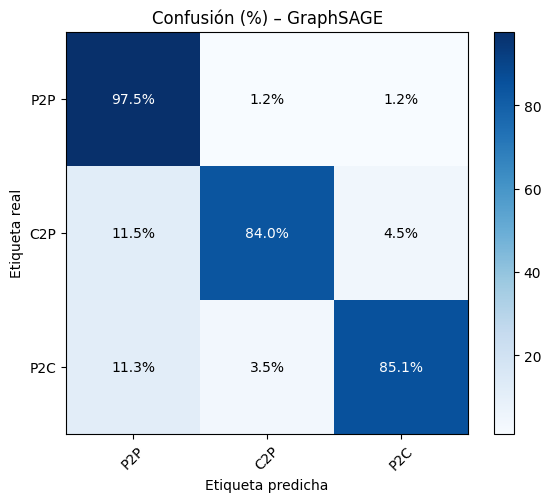
\includegraphics[width=\linewidth]{img//resultados//gnn//end-to-end//caso0/mc_graphsage_mlp_caso0.png}
%        \caption{Matriz de confusión – GraphSAGE}
        \label{fig:mc_graphsage_caso0}
    \end{minipage}
    \hfill
    \begin{minipage}[b]{0.32\linewidth}
        \centering
        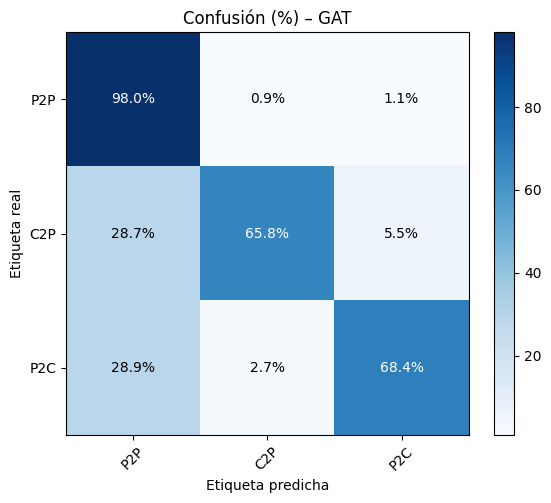
\includegraphics[width=\linewidth]{img//resultados//gnn//end-to-end//caso0/mc_gat_mlp_caso0.png}
%        \caption{Matriz de confusión – GAT}
        \label{fig:mc_gat_caso0}
    \end{minipage}
    \caption{Matrices de confusión obtenidas para el Caso 0 utilizando diferentes modelos GNN (GCN, GraphSAGE y GAT) con decodificador Bilinear.}

\end{figure}





\begin{figure}[H]
    \centering

    \begin{minipage}[b]{0.32\linewidth}
        \centering
        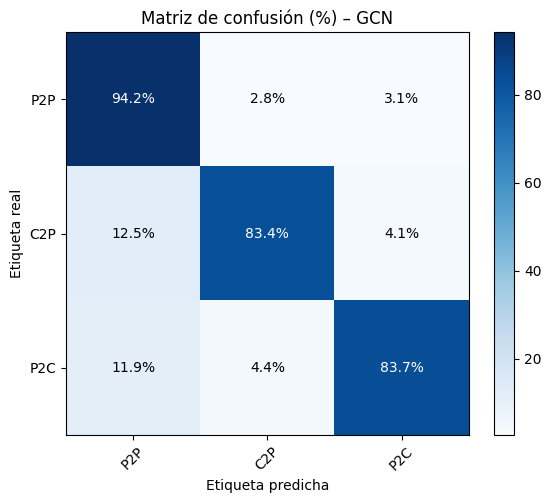
\includegraphics[width=\linewidth]{img//resultados//gnn//end-to-end//caso0/mc_gcn_mlp_caso0.png}
        % \caption{Matriz de confusión – GCN con MLP Early stop en epoch 110}
        \label{fig:mc_gcn_mlp_caso0}
    \end{minipage}
    \hfill
    \begin{minipage}[b]{0.32\linewidth}
        \centering
        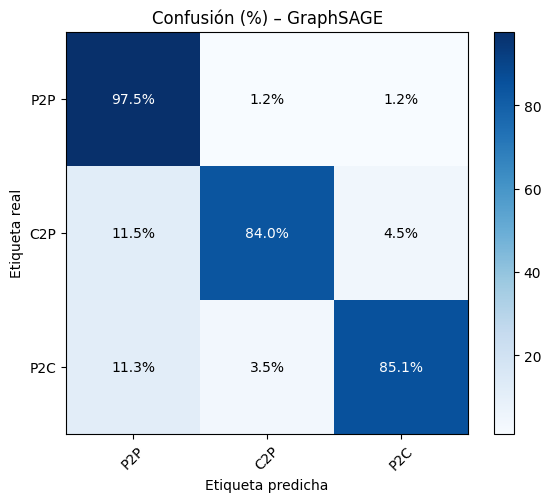
\includegraphics[width=\linewidth]{img//resultados//gnn//end-to-end//caso0/mc_graphsage_mlp_caso0.png}
        % \caption{Matriz de confusión – GraphSAGE con MLP Early stop en epoch 325}
        \label{fig:mc_graphsage_mlp_caso0}
    \end{minipage}
    \hfill
    \begin{minipage}[b]{0.32\linewidth}
        \centering
        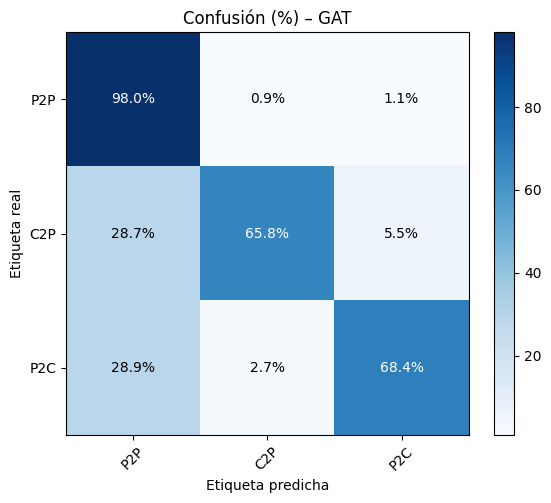
\includegraphics[width=\linewidth]{img//resultados//gnn//end-to-end//caso0/mc_gat_mlp_caso0.png}
        % \caption{Matriz de confusión – GAT con MLP Early stop en epoch 123}
        \label{fig:mc_gat_mlp_caso0}
    \end{minipage}
    \caption{Matrices de confusión obtenidas para el Caso 0 utilizando diferentes modelos GNN (GCN, GraphSAGE y GAT) con decodificador MLP.}

\end{figure}

Con este caso del enfoque \textit{end-to-end} podemos ver una clara mejora respecto al enfoque \textit{por etapas}. Las GNNs directamente sobre la tarea final (clasificación de relaciones económicas) permiten obtener representaciones de nodos más ajustadas al problema. La arquitectura GraphSAGE con decodificador MLP alcanza el mejor desempeño, con un Accuracy de 93,48\%, Precision 91\% y Recall 90\%.\\



% Para ver si lo sbuenos rusltados s trataban por los attributos se corrio l xprimnto 5 , donde se diron attr alatorios a cada nodo y lugo s ntrno.\\



\subsubsection{Caso 1: Se utiliza grafo con atributos de grado de entrada y salida}

\begin{itemize}
    \item \textbf{RIBs:} Febrero 2024.
    \item \textbf{Atributos de nodos:} Grado de entrada y salida de cada nodo.
    \item \textbf{Epochs:} 100.
    \item \textbf{Early Stopping:} Paciencia de 8 epochs.
    \item \textbf{Learning Rate:} 0,01.
\end{itemize}


Se entrena el modelo utilizando únicamente el decoder MLP, decisión que se tomó luego de ver los resultados obtenidos en el Caso 0, donde este alcanzó el mejor desempeño. A diferencia del caso anterior, se utilizan como atributos de los nodos solo el grado de entrada y el grado de salida de cada Sistema Autónomo.\\


\begin{figure}[H]
    \centering

    \begin{minipage}[b]{0.32\textwidth}
        \centering
        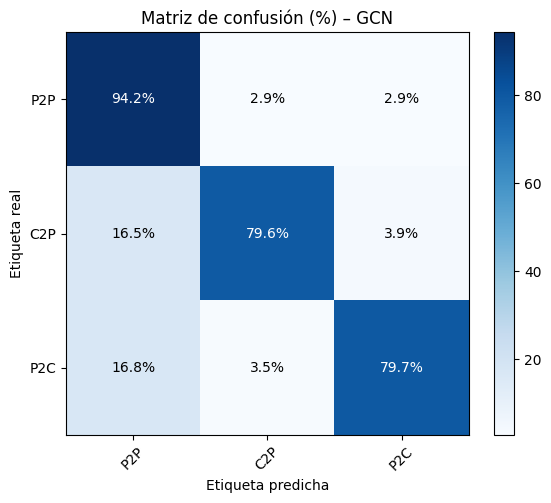
\includegraphics[width=\linewidth]{img//resultados//gnn//end-to-end//caso2/mc_bi_gcn.png}
%        \caption{GCN con decodificador bilineal}
        \label{fig:mc_bi_gcn}
    \end{minipage}
    \hfill
    \begin{minipage}[b]{0.32\textwidth}
        \centering
        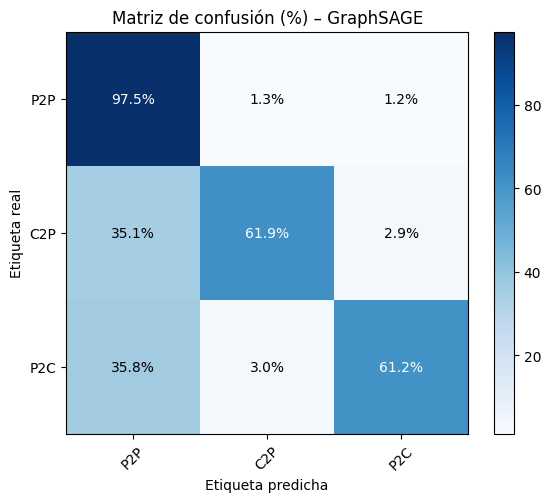
\includegraphics[width=\linewidth]{img//resultados//gnn//end-to-end//caso2/mc_bi_graphsage.png}
 %       \caption{GraphSAGE con decodificador bilineal}
        \label{fig:mc_bi_graphsage}
    \end{minipage}
    \hfill
    \begin{minipage}[b]{0.32\textwidth}
        \centering
        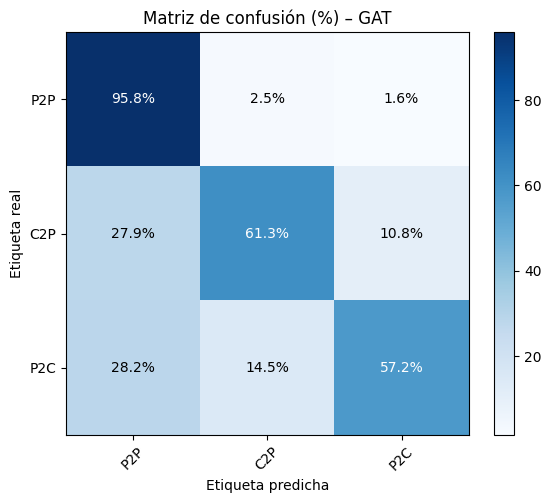
\includegraphics[width=\linewidth]{img//resultados//gnn//end-to-end//caso2/mc_bi_gat.png}
 %       \caption{GAT con decodificador bilineal}
        \label{fig:mc_bi_gat}
    \end{minipage}
    \caption{Matrices de confusión obtenidas para el Caso 1 utilizando diferentes modelos GNN (GCN, GraphSAGE y GAT) con decodificador MLP.}
\end{figure}




\begin{table}[H]
\centering
\begin{tabular}{lcccc}
\toprule
\textbf{Modelo} & \textbf{Precision (\%)}  & \textbf{Recall (\%)}  & \textbf{Accuracy (\%)} \\
\midrule
GCN        & \textbf{85.90} & \textbf{82.82} & \textbf{89.01} \\
GraphSAGE  & 84.76 & 67.92 & 83.44 \\
GAT        & 73.97 & 72.53 & 82.70 \\
\bottomrule
\end{tabular}
\caption{Resultados de clasificación por modelo utilizando decodificador MLP.}
\label{tab:caso1_mlp}
\end{table}




A pesar de utilizar atributos básicos como el grado de entrada y salida, este enfoque logra resultados competitivos, donde se alcanza un 89\% de Accuracy. Sin embargo, el resultado es inferior al caso 0 donde se trabaja con los atributos obtenidos de PeeringDB, lo que confirma que la calidad de los atributos  nodales es importante para obtener resultados superiores en la inferencia de relaciones económicas entre ASes. 




\subsubsection{Caso 2: Enfoque \textit{end-to-end} utilizando grafo con atributos de PeeringDB y muestreo aleatorio de vecinos (Random Neighbour Sampling)}

\begin{itemize}
    \item \textbf{RIBs:} Febrero 2024.
    \item \textbf{Atributos de nodos:} Dataset creado a partir de PeeringDB.
    \item \textbf{Esquema de entrenamiento:} Por \textit{batches}, aplicando \textit{Random Neighbour Sampling} en cada capa.
    \item \textbf{Epochs:}  100
    \item \textbf{Configuraciones evaluadas:} 5, 10, 15 y 20 vecinos por capa.
    \item \textbf{Early stopping:} Paciencia de 8 epochs.
    \item \textbf{Learning rate:} 0,01.
\end{itemize}








\begin{table}[H]
\centering
\caption{Desempeño de arquitecturas GNN con diferentes cantidades de vecinos aleatorios por capa.}
\label{tab:resultados_random_neighbors_resumen}
\resizebox{0.85\textwidth}{!}{
\begin{tabular}{lccccc}
\toprule
\textbf{Modelo} & \textbf{Vecinos} & \textbf{Precision (\%)} & \textbf{Recall (\%)} & \textbf{Accuracy (\%)} \\
\midrule
GCN        & 5  & 81.09 & 66.65 & 82.26 \\
GraphSAGE  & 5  & 81.55 & 58.95 & 79.68 \\
GAT        & 5  & 75.31 & 68.74 & 81.33 \\
\midrule
GCN        & 10 & 88.84 & 76.85 & 88.17 \\
GraphSAGE  & 10 & 87.60 & 80.94 & 89.38 \\
GAT        & 10 & 86.41 & 81.88 & 89.24 \\
\midrule
GCN        & 15 & 90.57 & 80.89 & 90.12 \\
GraphSAGE  & 15 & 90.90 & 81.89 & 90.56 \\
GAT        & 15 & 89.29 & 82.41 & 90.39 \\
\midrule
GCN        & 20 & \textbf{90.85} & \textbf{86.25} & \textbf{92.18} \\
GraphSAGE  & 20 & 90.46 & 85.35 & 91.78 \\
GAT        & 20 & 90.57 & 85.44 & 91.78 \\
\bottomrule
\end{tabular}
}
\end{table}

% ------------------------------------------
\begin{figure}[H]
    \centering

    \begin{minipage}[b]{0.32\textwidth}
        \centering
        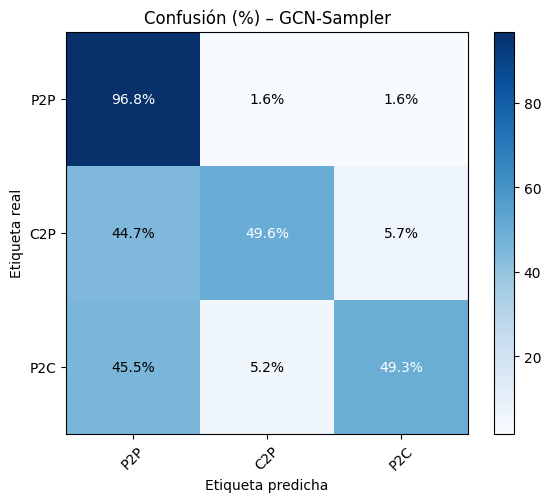
\includegraphics[width=\linewidth]{img//resultados//gnn//end-to-end//caso3/mc_gcn_mlp.png}
        % \caption{GCN con decoder MLP (5 vecinos)}
        \label{fig:mc_gcn_mlp_5nei}
    \end{minipage}
    \hfill
    \begin{minipage}[b]{0.32\textwidth}
        \centering
        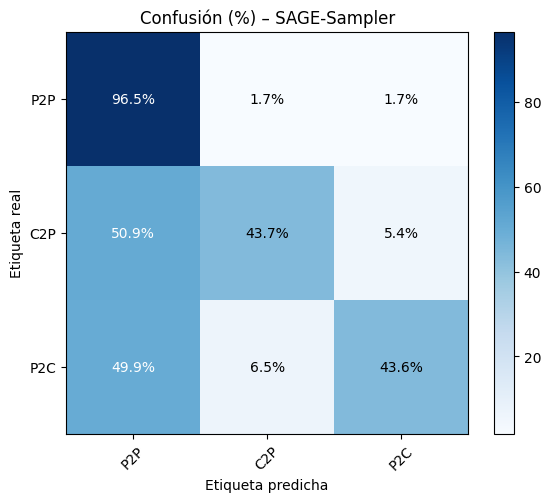
\includegraphics[width=\linewidth]{img//resultados//gnn//end-to-end//caso3/mc_graphsage_mlp.png}
        % \caption{GraphSAGE con decoder MLP (5 vecinos)}
        \label{fig:mc_graphsage_mlp_5nei}
    \end{minipage}
    \hfill
    \begin{minipage}[b]{0.32\textwidth}
        \centering
        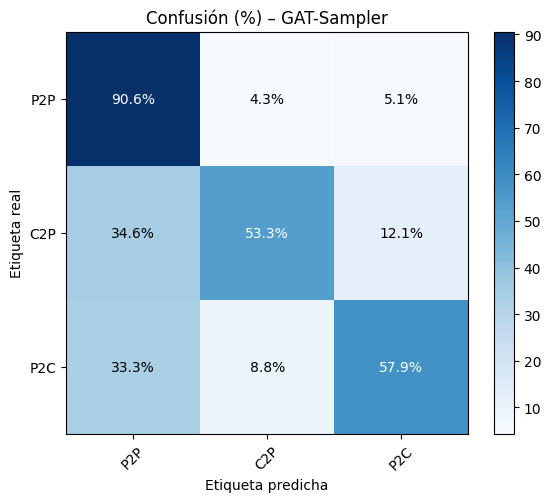
\includegraphics[width=\linewidth]{img//resultados//gnn//end-to-end//caso3/mc_gat_mlp.png}
        % \caption{GAT con decoder MLP (5 vecinos)}
        \label{fig:mc_gat_mlp_5nei}
    \end{minipage}
    \caption{Matrices de confusión obtenidas utilizando diferentes modelos GNN (GCN, GraphSAGE y GAT) con decodificador MLP y muestreo aleatorio de 5 vecinos por capa. }

 \end{figure}

% ------------------------------------------
\begin{figure}[H]
    \centering

    \begin{minipage}[b]{0.32\textwidth}
        \centering
        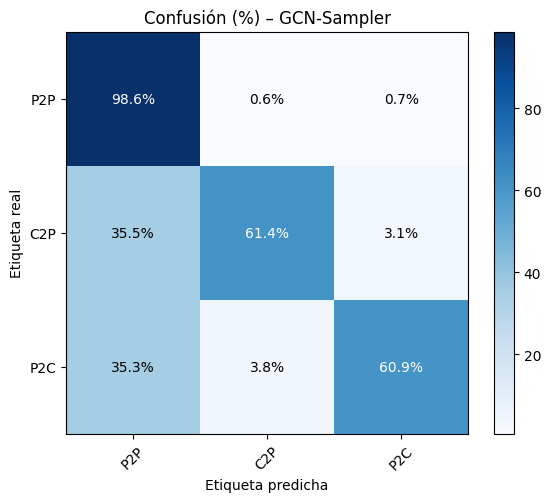
\includegraphics[width=\linewidth]{img//resultados//gnn//end-to-end//caso3/mc_gcn_mlp_10nei.png}
        %\caption*{(a) GCN con decoder MLP — Early stopping en epoch 15}        
        \label{fig:mc_gcn_mlp_10nei}
    \end{minipage}
    \hfill
    \begin{minipage}[b]{0.32\textwidth}
        \centering
        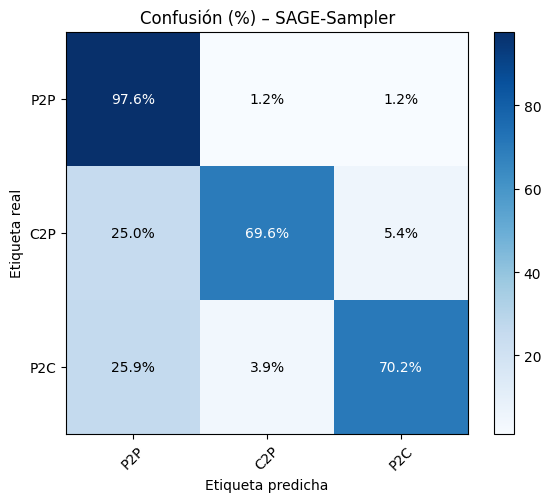
\includegraphics[width=\linewidth]{img//resultados//gnn//end-to-end//caso3/mc_graghsage_mlp_10nei.png}
       %\caption*{(b) GraphSAGE con decoder MLP — Early stopping en epoch 23}        
        \label{fig:mc_graphsage_mlp_10nei}
    \end{minipage}
    \hfill
    \begin{minipage}[b]{0.32\textwidth}
        \centering
        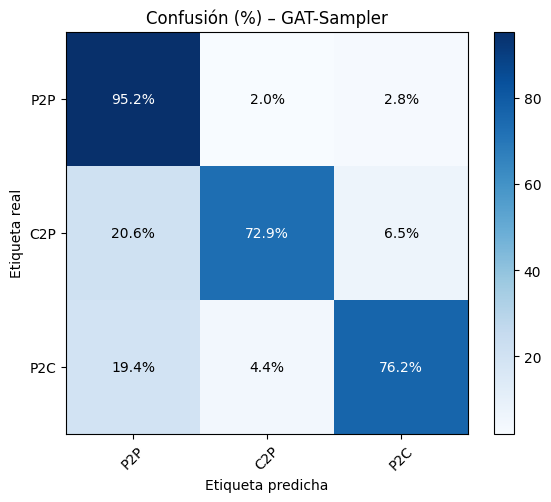
\includegraphics[width=\linewidth]{img//resultados//gnn//end-to-end//caso3/mc_gat_mlp_10nei.png}
        %\caption*{(c) GAT con decoder MLP — Early stopping en epoch 38}  
        \label{fig:mc_gat_mlp_10nei}
    \end{minipage}
    
    \caption{Matrices de confusión obtenidas utilizando diferentes modelos GNN (GCN, GraphSAGE y GAT) con decodificador MLP y muestreo aleatorio de 10 vecinos por capa. }
\end{figure}
% ------------------------------------------

\begin{figure}[H]
    \centering

    \begin{minipage}[b]{0.32\textwidth}
        \centering
        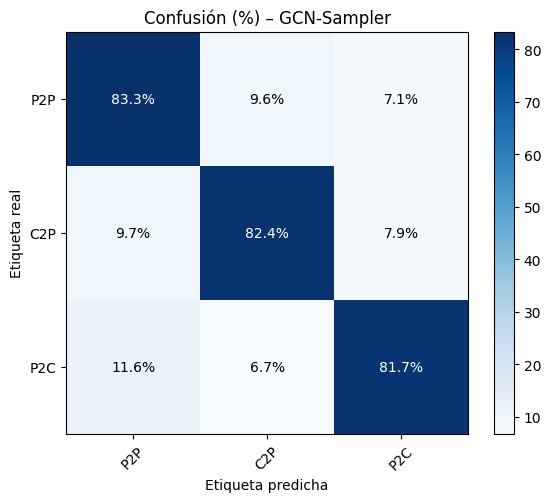
\includegraphics[width=\linewidth]{img//resultados//gnn//end-to-end//caso3/mc_gcn_mlp_15nei.png}
        % \caption{GCN con decoder MLP (15 vecinos)}
        \label{fig:mc_gcn_mlp_15nei}
    \end{minipage}
    \hfill
    \begin{minipage}[b]{0.32\textwidth}
        \centering
        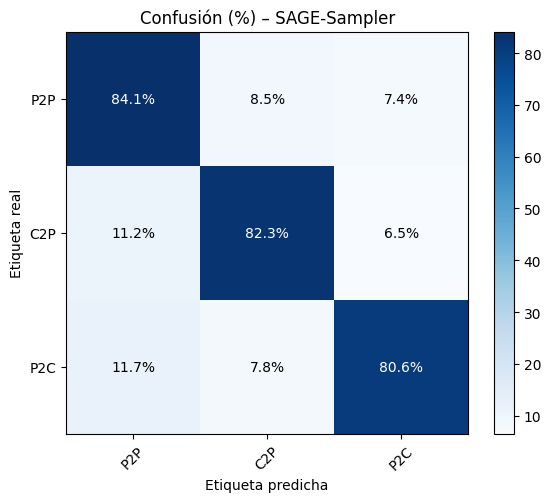
\includegraphics[width=\linewidth]{img//resultados//gnn//end-to-end//caso3/mc_graphsage_mlp_15nei.png}
        % \caption{GraphSAGE con decoder MLP (15 vecinos)}
        \label{fig:mc_graphsage_mlp_15nei}
    \end{minipage}
    \hfill
    \begin{minipage}[b]{0.32\textwidth}
        \centering
        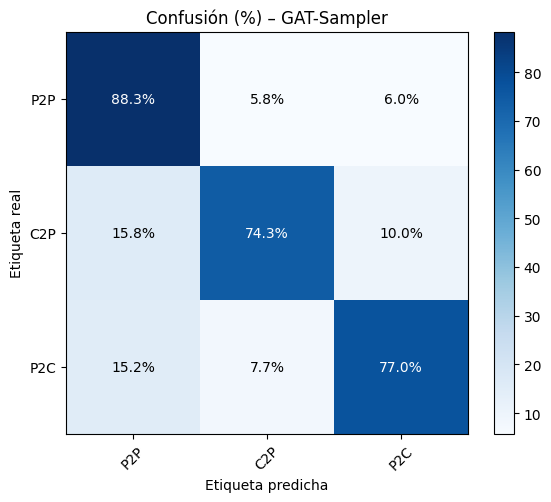
\includegraphics[width=\linewidth]{img//resultados//gnn//end-to-end//caso3/mc_gat_mlp_15nei.png}
        % \caption{GAT con decoder MLP (15 vecinos)}
        \label{fig:mc_gat_mlp_15nei}
    \end{minipage}
    \caption{Matrices de confusión obtenidas utilizando diferentes modelos GNN (GCN, GraphSAGE y GAT) con decodificador MLP y muestreo aleatorio de 15 vecinos por capa. }
\end{figure}

% ------------------------------------------

\begin{figure}[H]
    \centering

    \begin{minipage}[b]{0.32\linewidth}
        \centering
        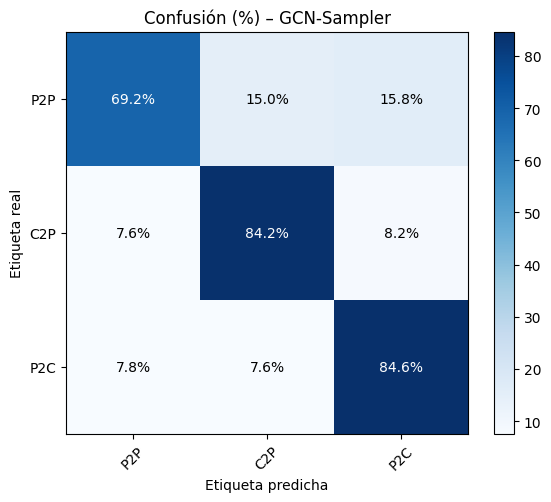
\includegraphics[width=\linewidth]{img//resultados//gnn//end-to-end//caso3/mc_gcn_mlp_20nei.png}
        % \caption*{GCN + MLP}
        \label{fig:mc_gcn_mlp_20nei}
    \end{minipage}
    \hfill
    \begin{minipage}[b]{0.32\linewidth}
        \centering
        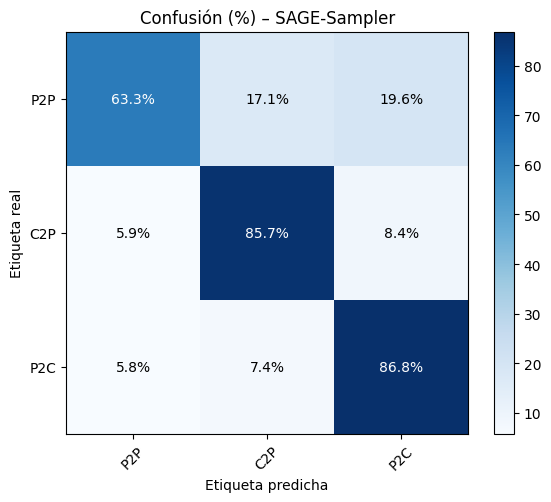
\includegraphics[width=\linewidth]{img//resultados//gnn//end-to-end//caso3/mc_graphsage_mlp_20neig.png}
        % \caption*{GraphSAGE + MLP}
        \label{fig:mc_graphsage_mlp_20nei}
    \end{minipage}
    \hfill
    \begin{minipage}[b]{0.32\linewidth}
        \centering
        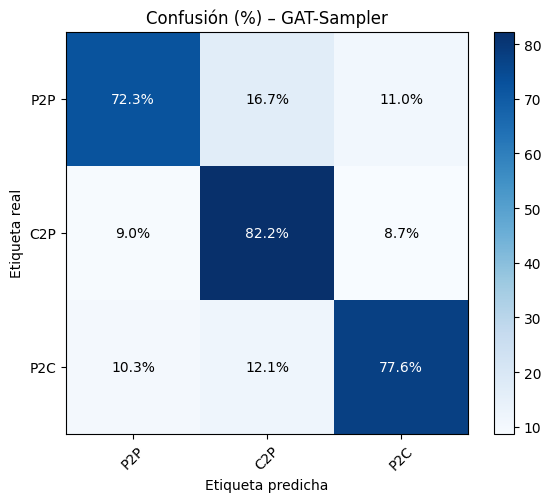
\includegraphics[width=\linewidth]{img//resultados//gnn//end-to-end//caso3/mc_gat_mlp_20nei.png}
        % \caption*{GAT + MLP}
        \label{fig:mc_gat_mlp_20nei}
    \end{minipage}

    \caption{Matrices de confusión para GCN, GraphSAGE y GAT usando decodificador MLP con 20 vecinos aleatorios por capa.}
    \label{fig:mc_gnns_mlp_20nei}
\end{figure}


Se logra ver que el uso de muestreo aleatorio de vecinos es una alternativa eficiente para entrenar modelos GNN en grafos grandes, permitiendo reducir la carga computacional sin sacrificar demasiado rendimiento. 
Específicamente para nuestro escenario, GCN alcanza el mejor resultado con una Accuracy de 92.18\%. El mejor resultado se obtiene con 20 vecinos, lo que nos dice que el muestreo de un mayor número de vecinos permite capturar más contexto estructural, reduciendo la pérdida de información.\\

%A medida que se incrementa la cantidad de vecinos muestreados por capa, se observa una mejora en el desempeño de los modelos, especialmente en la clasificación de las clases minoritarias (C2P y P2C). Con 10 y 15 vecinos, los modelos logran un mejor balance entre Precision y recall. Sin embargo, al llegar a 20 vecinos, el rendimiento disminuye en algunos casos, probablemente por información redundante o ruido. GAT se muestra más robusto ante este aumento, gracias a su mecanismo de atención, mientras que GraphSAGE es más sensible a este cambio.\\

%El modelo GAT aprovecha mejor el hecho de tener más vecinos gracias a su mecanismo de atención, que le permite asignar distintos pesos a cada nodo y priorizar la información más relevante. En cambio, GraphSAGE combina directamente la información de sus vecinos mediante agregación, lo que puede ser más perjudicial en escenarios con muestreo aleatorio, ya que no existe un criterio topológico para seleccionar vecinos y esto puede llevar a un muestreo poo representativo.\\


\subsubsection{Caso 3: Se utiliza grafo con atributos de PeeringDB y muestreo basado en comunidades (ClusterGCN)}

\begin{itemize}
    \item \textbf{RIBs:} Febrero 2024.
    \item \textbf{Atributos de nodos:} Dataset creado a partir de PeeringDB.
    \item \textbf{Esquema de entrenamiento:} Por \textit{batches}, aplicando \textit{ClusterGCN}.
    \item \textbf{Epochs:} 100.
    \item \textbf{Configuraciones evaluadas:} Tamaño de  clúster de 1000 nodos.    
    \item \textbf{Early Stopping:} Paciencia de 8 epochs.
    \item \textbf{Learning rate:} 0,01.
\end{itemize}


ClusterGCNSampler es un estrategia de muestreo que divide el grafo en clusters, y entrena usando mini-batches basados en esos subgrafos en lugar de todo el grafo.\\


\begin{table}[H]
\centering

\begin{tabular}{lcccc}
\toprule
\textbf{Modelo} & \textbf{Precision (\%)}  & \textbf{Recall (\%)} & \textbf{Accuracy (\%)} \\
\midrule
GCN & \textbf{89.16} & \textbf{89.21} & \textbf{89.16} \\
GraphSAGE & 89.16 & 89.22 & 89.11 \\
GAT & 79.92 & 78.40 & 78.54 \\
\bottomrule
\end{tabular}

\caption{Resultados de clasificación por modelo utilizando decodificador MLP con muestreo basado en comunidades (\textit{ClusterGCN}).}

\label{tab:caso3_mlp_clustergcn}
\end{table}




\begin{figure}[H]
    \centering
        \centering
        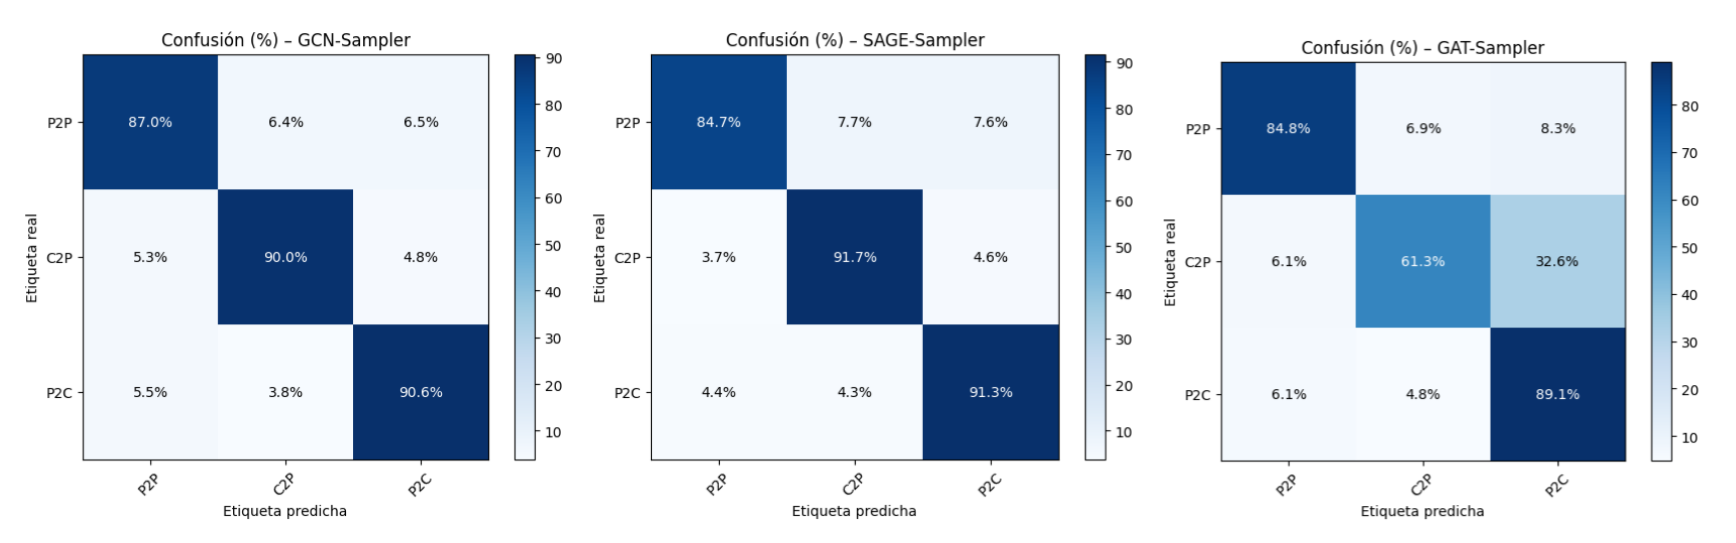
\includegraphics[width=\linewidth]{img//resultados//gnn//end-to-end//casoclustrgcn/clusterGCNMatrices.png}
        %\caption{GCN + MLP con ClusterGCN}
        \label{fig:mc_gcn_cluster}
    \caption{Matrices de confusión obtenidas utilizando diferentes modelos GNN (GCN, GraphSAGE y GAT) con decodificador MLP y clúster tamaño 10000.}
\end{figure}




Este caso demuestra que el muestreo por comunidades (ClusterGCN) es una opción viable para escalar en grafos grandes. Sin embargo, los resultados son inferiores a los obtenidos con full batch, lo que sugiere un trade-off entre escalabilidad y métricas de desempeño del modelo. Además, se observa que GAT pierde capacidad discriminatoria bajo este esquema.\\


%En comparación a los otros casos, el enfoque con ClusterGCN muestra un rendimiento intermedio. Aunque GCN y GraphSAGE alcanzan buenos resultados (87,83\% y 88,10\% de accuracy, respectivamente), estos son inferiores a los obtenidos en el Caso 0 (con atributos ricos de PeeringDB y entrenamiento full-batch), donde los mismos modelos superan el 92\% de accuracy. Esto sugiere que, si bien ClusterGCN permite escalar a grafos grandes con eficiencia, puede perder parte del contexto global al segmentar la topología del grafo en subgrafos desconectados.



%hay arly stopying n poch 40
 %En contraste, los resultados superan claramente a los del Caso 1, donde los nodos solo contaban con información de grado, y también son más estables que en el Caso 2 con muestreo aleatorio, especialmente para GAT, que presenta una degradación considerable con 20 vecinos. 
 
%     GCN clásico requiere toda la vecindad de cada nodo → no es batchable naturalmente.

%     ClusterGCN lo resuelve permitiendo entrenamiento por subgrafos precomputados.

% 3. Subgrafos más informativos

%     A diferencia del muestreo aleatorio (e.g., en GraphSAGE), los clusters suelen estar estructuralmente conectados, preservando mejor la topología del grafo.

    

%     Subgrafos más densos → mejores señales de entrenamiento.

%     Menos variabilidad por sampling → más estable que random neighbors.






% Algunas razones posibles son:

%     El modelo es simple o no tiene suficiente capacidad para sobreajustar incluso si quisiera (por ejemplo, pocas capas o parámetros).

%     El problema es fácil o las clases están bien separadas, por lo que el modelo no necesita memorizar ejemplos específicos.

%     Los conjuntos de entrenamiento y validación son muy similares (por ejemplo, por cómo hiciste el split, o si hay mucha redundancia entre ambos).

%     Regularización efectiva: Puede que uses dropout, weight decay o alguna técnica que evita el overfitting de forma natural.

%     Cantidad de datos: Si tienes muchos datos y el modelo es pequeño, es difícil que sobreentrene.






\subsubsection{Caso 4: Se utiliza grafo con atributos de nodos generados aleatoriamente}



\begin{itemize}
    \item \textbf{RIBs:} Febrero 2024.
    \item \textbf{Atributos de nodos:} Atributos generados aleatoriamente, tamaño 32.
    \item \textbf{Epochs:} 100. 
    \item \textbf{Early Stopping:} Paciencia de 10 epochs.
    \item \textbf{Learning Rate:} 0.01.
\end{itemize}


El objetivo fue evaluar cómo se comporta el modelo cuando los atributos de los nodos no contienen información estructural ni semántica. Para esto se generaron atributos aleatorios para los nodos del grafo con el fin de evaluar si la información estructural del grafo por sí sola es suficiente para realizar la tarea de inferencia y así comparar con los casos anteriores y analizar que tan importantes son los atributos utilizados previamente.\\



\begin{table}[H]
\centering
\begin{tabular}{lcccc}
\toprule
\textbf{Modelo} & \textbf{Precision (\%)} & \textbf{Recall (\%)}  & \textbf{Accuracy (\%)} \\
\midrule
GCN & \textbf{85.75} & \textbf{74.68} & \textbf{85.85} \\
GraphSAGE & 56.19 & 33.34 & 68.56\\
GAT & 63.02 & 61.86 & 77.73 \\
\bottomrule
\end{tabular}

\caption{Resultados de clasificación por modelo utilizando decodificador MLP. En Precision, recall y F1-score se muestran los valores promedio macro (clases 0, 1 y 2).}
\label{tab:caso4_mlp_random_attr}
\end{table}

\begin{figure}[H]
    \centering
    \begin{minipage}{0.32\textwidth}
        \centering
        
\includegraphics[width=\linewidth]{img//resultados//gnn//end-to-end//casorandom/mc_gcn_mlp.png}
  %      \caption*{GCN + MLP}
        \label{fig:mc_gcn_random}
    \end{minipage}\hfill
    \begin{minipage}{0.32\textwidth}
        \centering
        
\includegraphics[width=\linewidth]{img//resultados//gnn//end-to-end//casorandom/mc_graphsage_mlp.png}
 %       \caption*{GraphSAGE + MLP}
        \label{fig:mc_graphsage_random}
    \end{minipage}\hfill
    \begin{minipage}{0.32\textwidth}
        \centering
        
\includegraphics[width=\linewidth]{img//resultados//gnn//end-to-end//casorandom/mc_gat_mlp.png}
%        \caption*{GAT + MLP}
        \label{fig:mc_gat_random}
    \end{minipage}
    \caption{Matrices de confusión obtenidas utilizando modelos GCN, GraphSAGE y GAT con decodificador MLP con atributos aleatorios.}
    \label{fig:mc_random_all}
\end{figure}

Los resultados muestran que GCN es el único que alcanza resultados aceptables con una Accuracy de 85,9\% , mientras que GraphSAGE y GAT colapsan hacia la predicción trivial de la clase mayoritaria (P2P), sin lograr discriminar las clases C2P y P2C. Esto se debe a cómo cada arquitectura procesa la información; GCN utiliza una matriz de adyacencia, que le permite capturar patrones estructurales del grafo incluso en ausencia de atributos significativos. En cambio, GraphSAGE y GAT dependen fuertemente de la agregación de atributos de los vecinos y como en estos experimentos los atributos son aleatorios resulta en que los modelos predigan siempre la misma clase superior (P2P). Con esto podemos decir que, si bien la estructura del grafo por sí sola contiene información suficiente para que GCN mantenga un desempeño razonable, los atributos tienen un rol importante en las arquitecturas GNN. Por lo tanto, el uso de atributos resulta esencial para explotar plenamente el potencial de estos modelos en la inferencia de relaciones económicas.\\



%Los resultados muestran que GCN es el único modelo que alcanza un rendimiento aceptable, con una accuracy de 85,9%, mientras que GraphSAGE y GAT colapsan hacia la predicción trivial de la clase mayoritaria (P2P), sin lograr discriminar las clases C2P y P2C. Esto se debe a la forma en que cada arquitectura procesa la información: GCN utiliza una matriz de adyacencia normalizada, lo que le permite capturar patrones estructurales del grafo incluso en ausencia de atributos significativos. En cambio, GraphSAGE y GAT dependen fuertemente de la agregación de atributos de los vecinos y, dado que en este experimento los atributos son aleatorios, los embeddings resultan poco diferenciados, llevando a los modelos a predecir siempre la clase dominante (P2P). Con ello podemos concluir que, si bien la estructura del grafo por sí sola contiene información suficiente para que GCN mantenga un desempeño razonable, los atributos de los nodos juegan un rol fundamental en arquitecturas más complejas. Por lo tanto, el uso de atributos informativos resulta esencial para explotar plenamente el potencial de los modelos GNN en la inferencia de relaciones económicas.








%/////////////////////////////////////////////////
\section{Resultados del \textit{Benchmark} de métodos tradicionales} \label{sec:benchmark_result_section}

Para la inferencia de las relaciones comerciales entre Sistemas Autónomos, primero se ejecutaron los distintos métodos sobre los datos correspondientes a las fechas en que se recolectaron las RIBs. Para esto se ocuparon las primeras $1.000.000$ de rutas de \texttt{sanitized\_ribs.txt}. Como el dataset de evaluación (CAIDA AS Relationships) se ocuparía para métodos de deep learning, se tuvo que dividir en conjuntos de entrenamiento y evaluación. Además, este mismo dataset de evaluación se utilizó para evaluar todos los métodos, con el fin de mantener la consistencia en la comparación de los resultados. \\

\begin{figure}[H]
    \centering

    \begin{subfigure}[h]{0.48\textwidth}
        \centering
        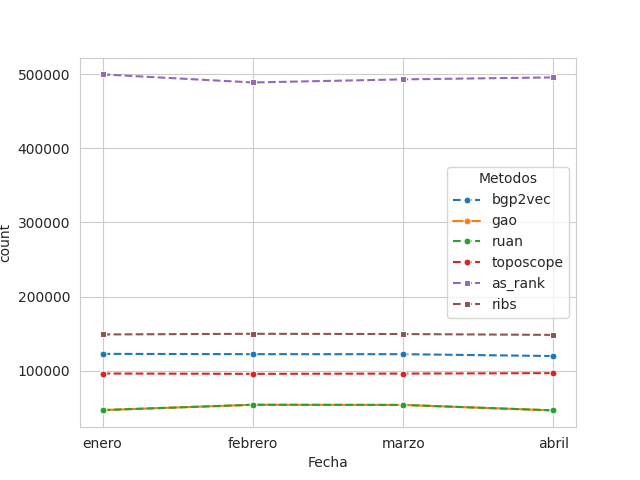
\includegraphics[width=\textwidth]{img/resultados/comparacion_metodos_cantidad.png}
        \caption{Cantidad de relaciones de los métodos para diferentes fechas.}
        \label{fig:comparacion_metodos_cantidad}
    \end{subfigure}
    \hfill
    \begin{subfigure}[h]{0.48\textwidth}
        \centering
        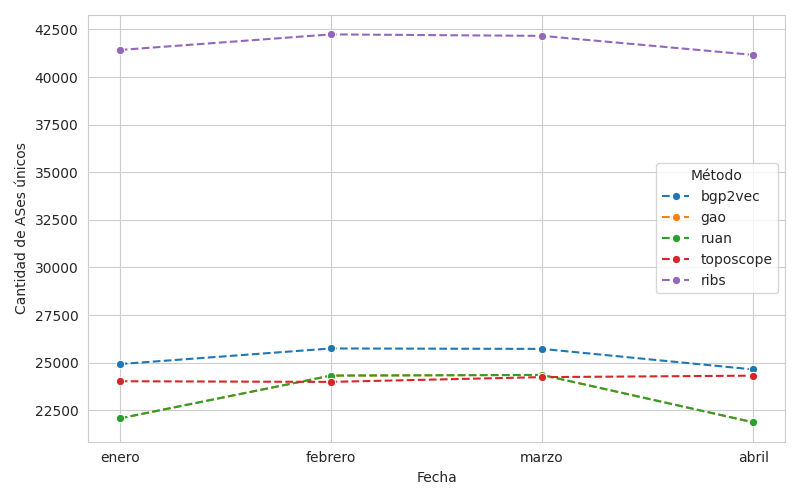
\includegraphics[width=\textwidth]{img/resultados/comparacion_metodos_cantidad_ASes.png}
        \caption{Cantidad de ASes de los métodos para diferentes fechas.}
        \label{fig:comparacion_metodos_cantidad_ASes}
    \end{subfigure}

    \caption{Cantidad de aristas inferidas y cantidad de ASes inferidos por cada método para distintas fechas.}


\end{figure}

Por esta razón, en la Figuras ~\ref{fig:comparacion_metodos_cantidad}  y \ref{fig:comparacion_metodos_cantidad_ASes} se muestran la cantidad de ASes y aristas inferidas por cada método, pues puede haber aristas que fueron inferidas pero no están presentes en el dataset de evaluación, así como aristas que sí están en el dataset pero no fueron inferidas por algunos métodos, lo cual es de esperarse dada la naturaleza del problema y las diferencias en los enfoques utilizados. Como era de esperarse, bgp2vec es el método que infiere la mayor cantidad de relaciones, ya que infiere todas las relaciones que se le proporcionan en el conjunto de test.\\


Se analizaron los enlaces inferidos y se vio si estos se mantenían constantes a lo largo de los distintos meses. Sin embargo, dado que solo se pudo utilizar una porción de las RIBs, los paths disponibles varían entre meses, lo que provocó que algunas relaciones estuvieran presentes en un mes pero ausentes en otros. Como resultado, el número de relaciones que coincidían en los cuatro meses fue muy reducido. Sin embargo, si se considera que una relación se mantiene constante si aparece en al menos dos meses, se obtiene la distribución presentada en la Figura~\ref{fig:relaciones_constantes_cambiantes_por_metodo}, donde en naranjo aparece la cantidad de enlaces que aparecen iguales en los cuatro meses en los que se ejecutaron los diferentes métodos y en rojo la cantidad que fue cambiando.\\

\begin{figure}[H]
    \centering
    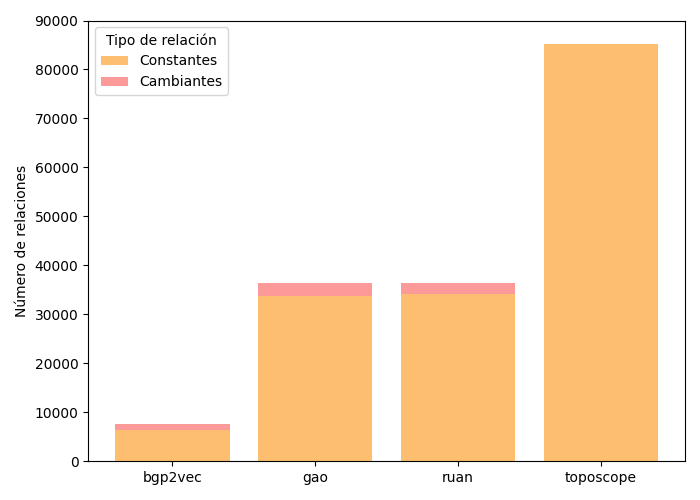
\includegraphics[width=0.7\textwidth]{img/resultados/relaciones_constantes_cambiantes_por_metodo.png}
    
    \caption{Constancia de relaciones con el tiempo}
    \label{fig:relaciones_constantes_cambiantes_por_metodo}
\end{figure}


\begin{table}[H]
\centering
\caption{Coincidencia entre métodos de inferencia en febrero}
\label{tab:comparacion_metodos_febrero}
\begin{tabular}{llrrr}
\toprule
Método 1 & Método 2 & Relaciones comparadas & Coincidencias & Porcentaje (\%) \\
\midrule
gao       & ruan       & 48.680 & 37.147 & 76.31 \\
gao       & toposcope  & 15.238 & 6.558  & 43.04 \\
gao       & bgp2vec    & 10     & 4      & 40.00 \\
ruan      & toposcope  & 15.238 & 3.922  & 25.74 \\
ruan      & bgp2vec    & 10     & 3      & 30.00 \\
toposcope & bgp2vec    & 13     & 6      & 46.15 \\
\bottomrule
\end{tabular}
\end{table}

La Tabla~\ref{tab:comparacion_metodos_febrero} muestra el grado de coincidencia entre distintos métodos de inferencia de relaciones AS durante el mes de febrero. Se observa una alta consistencia entre los métodos Gao y Ruan, con más del 76\% de coincidencias. En contraste con los métodos Toposcope y BGP2Vec que  presentan un menor grado de coincidencia, probablemente debido a diferencias metodológicas y a la cobertura de inferencia. La información presentada fue obtenida cruzando los \textit{datasets} de cada método para el mes de febrero, identificando las relaciones entre sistemas autónomos (AS) comunes entre pares de métodos.\\




Una vez ejecutados los diferentes métodos, se obtuvieron los valores de Accuracy que se presentan en la Tabla~\ref{tab:comparacion_accuracy}. 
%Los valores de Precision, Recall y F1-score correspondientes pueden encontrarse en las Tablas~\ref{tab:comparacion_presicion},  ~\ref{tab:comparacion_f1_score}, y ~\ref{tab:comparacion_recall} respectivamente, ubicadas en el Anexo~\ref{sec:bechmark_resultados}. \\


\begin{table}[H]
    \centering
    \begin{tabular}{lccccc}
    \hline
    \textbf{Método} & \textbf{Accuracy} \\
    \hline
    Gao & 81.77\% \\
    Ruan & 64.48\% \\
    ProbLink & 94.83\% \\
    TopoScope & 94.13\% \\
    bgp2vec & 94.51\% \\
    \hline
    \end{tabular}
    \caption{Comparación de resultados de \textit{Accuracy} entre distintos métodos.}
    \label{tab:comparacion_accuracy}
\end{table}

En la Figura~\ref{fig:relaciones_por_tipo_y_metodo} se muestra la cantidad de relaciones inferidas por tipo para cada uno de los métodos evaluados, donde claramente, bgp2vec es el método que infiere el mayor número de relaciones. Esto se debe a que su enfoque está basado en Machine Learning, el cual le permite inferir un tipo de relación para cada enlace presente en las rutas del conjunto de test. Además, se observa que bgp2vec tiende a inferir una gran cantidad de relaciones del tipo p2p. 
Por otro lado, Gao y Ruan infieren la misma cantidad total de relaciones, sin embargo, en esta figura se aprecia que, la distribución por tipo de relación es distinta.\\


\begin{figure}[H]
    \centering
    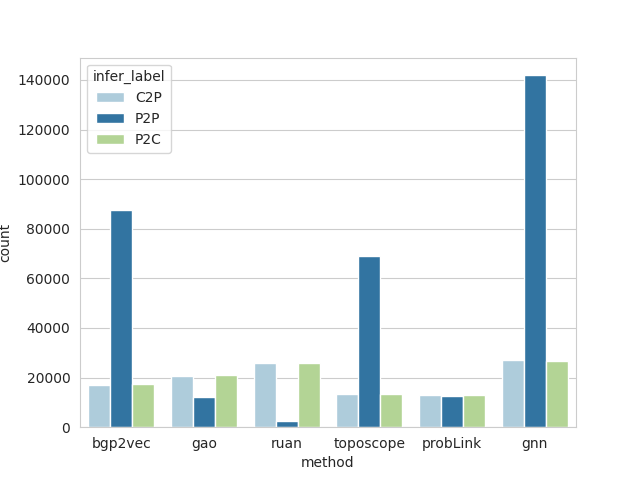
\includegraphics[width=0.7\textwidth]{img/resultados/benchmark/relaciones_por_tipo_y_metodo.png}
    \caption{Cantidad de relaciones por tipo para cada método para relaciones extraídas de RIBs de febrero de 2024.}
    \label{fig:relaciones_por_tipo_y_metodo}
\end{figure}


En las Figuras~\ref{fig:inferidos_correcta_icorrectamente_todo} y~\ref{fig:inferidos_correcta_icorrectamente_por_tipo} se presenta el conteo de relaciones inferidas correctamente e incorrectamente por cada método, y separadas por tipo, utilizando el conjunto de evaluación correspondiente a febrero de 2024.\\

\begin{figure}[H]
    \centering
    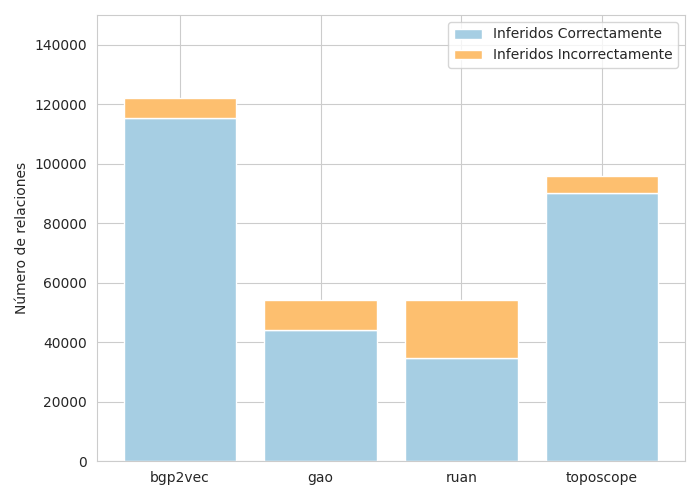
\includegraphics[width=0.7\textwidth]{img/resultados/inferidos_correcta_icorrectamente_todo.png}
    \caption{Cantidad de relaciones correctamente e incorrectamente inferidas por cada método para febrero de 2024.}
\label{fig:inferidos_correcta_icorrectamente_todo}
\end{figure}


\begin{figure}[H]
    \centering
    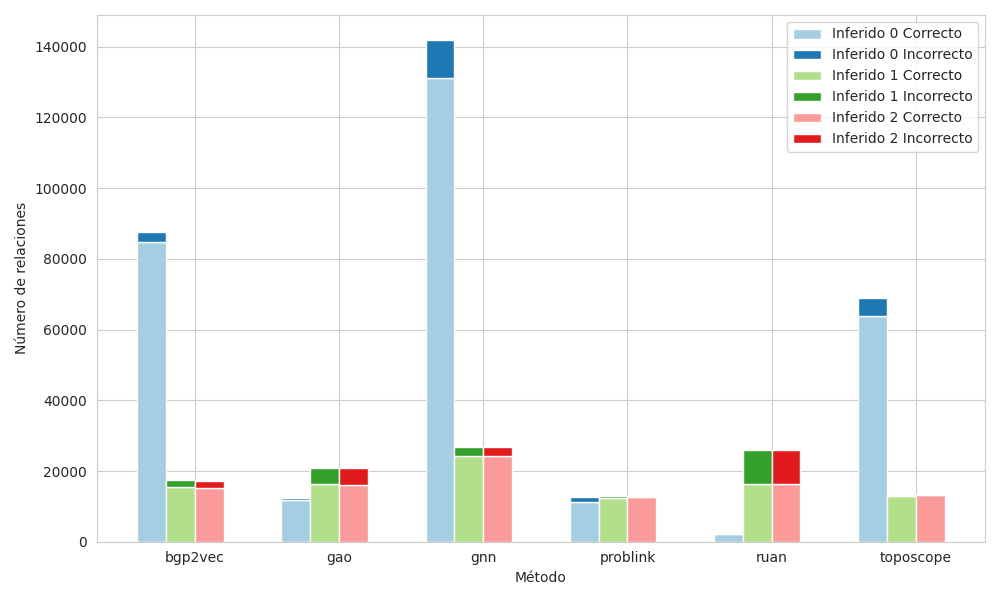
\includegraphics[width=0.8\textwidth]{img/resultados/benchmark/relaciones_inferidas_por_metodo_y_tipo.png}
    
    \caption{Cantidad de relaciones correctamente e incorrectamente inferidas, separadas por tipo, para febrero de 2024.}
    \label{fig:inferidos_correcta_icorrectamente_por_tipo}
\end{figure}

\newpage
Finalmente, al obtener las matrices de confusión para cada uno de los métodos, correspondientes al mes de febrero de 2024 (Figura~\ref{fig:comparacion-confusion}), se observa que las relaciones p2p son las más difíciles de inferir, ya que varios métodos tienden a confundirlas con c2p. Los métodos modernos como \textbf{ProbLink} y \textbf{TopoScope} ofrecen un mayor poder discriminativo, reduciendo significativamente la confusión entre pares P2P–C2P, mientras que los enfoques basados en \textit{embeddings} o heurísticas previas (BGP2Vec, Guo, Ruan) tienden a sobreclasificar las relaciones descendentes (c2p).




\begin{figure}[H]
    \centering

    \begin{subfigure}[t]{0.40\textwidth}
        \centering
        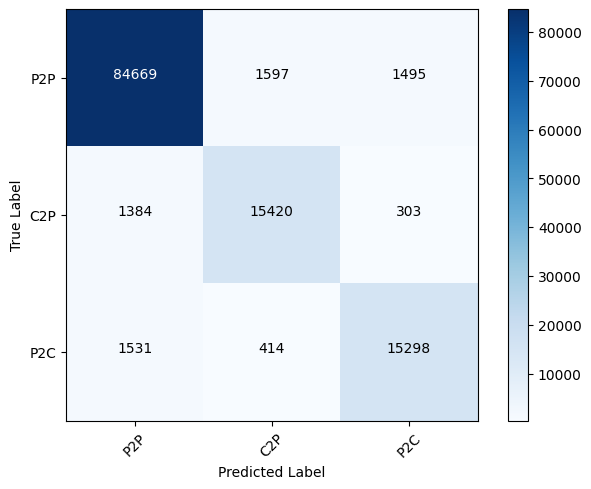
\includegraphics[width=\textwidth]{img/resultados/matrices_confusion/Confusion_matrix_bgp2vec_1m_febrero.png}
        \caption{BGP2Vec}
        \label{fig:confusion-bgp2vec}
    \end{subfigure}
    \hfill
    \begin{subfigure}[t]{0.4\textwidth}
        \centering
        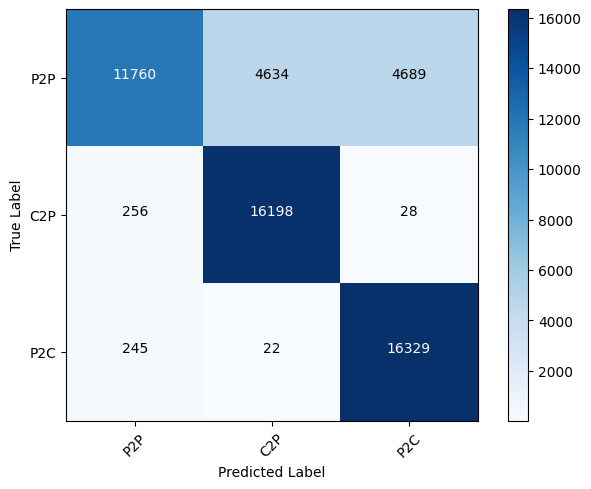
\includegraphics[width=\textwidth]{img/resultados/matrices_confusion/Confusion_matrix_gao_1m_febrero.png}
        \caption{Gao}
        \label{fig:confusion-gao}
    \end{subfigure}

    \vspace{0.75em}

    \begin{subfigure}[t]{0.4\textwidth}
        \centering
        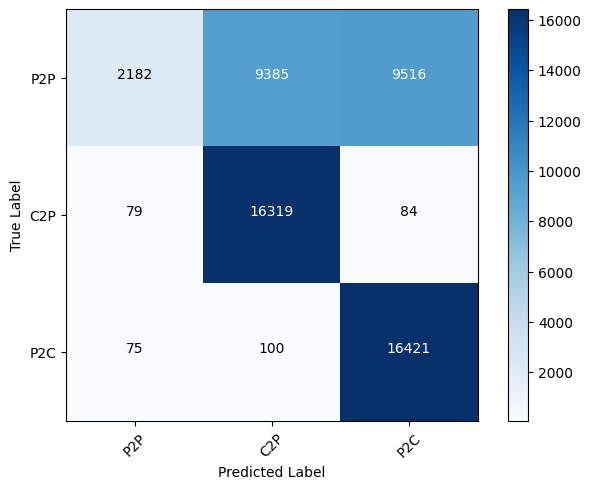
\includegraphics[width=\textwidth]{img/resultados/matrices_confusion/Confusion_matrix_ruan_1m_febrero.png}
        \caption{Ruan}
        \label{fig:confusion-ruan}
    \end{subfigure}
    \hfill
    \begin{subfigure}[t]{0.4\textwidth}
        \centering
        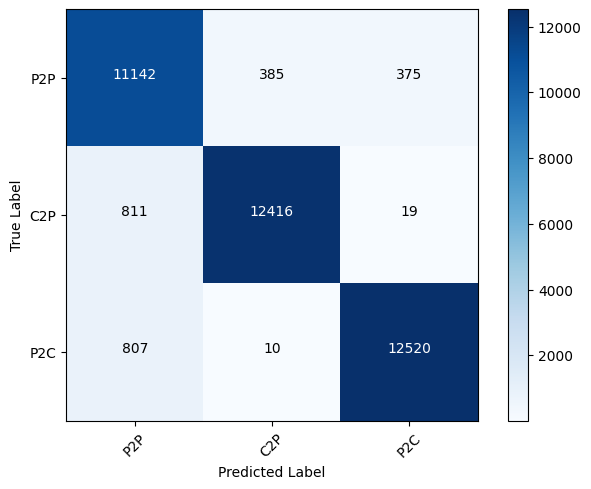
\includegraphics[width=\textwidth]{img/resultados/matrices_confusion/Confusion_matrix_problink_1m_febrero.png}
        \caption{ProbLink}
        \label{fig:confusion-problink}
    \end{subfigure}

    \vspace{0.75em}

    \begin{subfigure}[t]{0.4\textwidth}
        \centering
        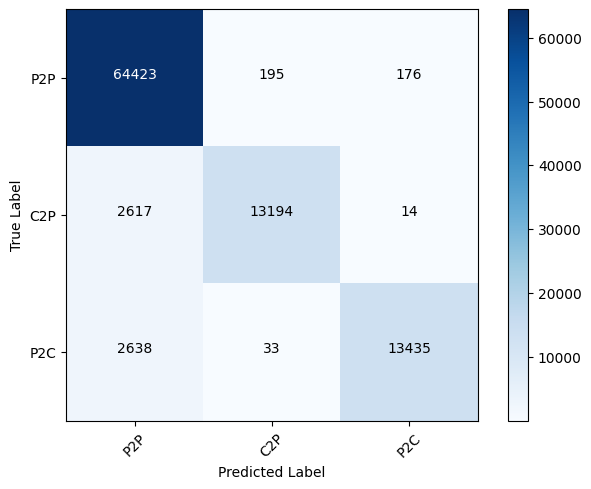
\includegraphics[width=\textwidth]{img/resultados/matrices_confusion/Confusion_matrix_toposcope_1m_febrero.png}
        \caption{TopoScope}
        \label{fig:confusion-toposcope}
    \end{subfigure}

    \caption{Matrices de confusión por método (febrero 2024).}
    \label{fig:comparacion-confusion}
\end{figure}


%El método GAO presenta una tendencia clara a confundir relaciones simétricas (P2P) con relaciones jerárquicas. En particular, se observan 4721 casos en que una relación P2P fue inferida como C2P, y 4636 casos en que fue clasificada como P2C. No obstante, el modelo demuestra alta Precision al inferir correctamente relaciones jerárquicas: 16.218 casos correctamente clasificados como C2P y 16.128 como P2C. Esto sugiere que GAO es un método confiable para la inferencia jerárquica, aunque tiende a subestimar la presencia de relaciones simétricas.\\


%Por su parte, el método RUAN presenta errores significativamente altos al momento de inferir relaciones P2P. Solo 2163 de estas relaciones fueron correctamente identificadas, mientras que más de 18.900 fueron clasificadas erróneamente como jerárquicas (9444 como C2P y 9502 como P2C). A pesar de esto, RUAN muestra un excelente rendimiento al clasificar relaciones jerárquicas, con 16.347 aciertos en C2P y 16.250 en P2C. Esta evidencia indica que RUAN comparte con GAO la fortaleza en jerarquías, pero presenta una marcada debilidad al reconocer relaciones simétricas.\\


%El método TOPOSCOPE presenta un comportamiento opuesto al de GAO y RUAN. Este clasificador tiende a sobreestimar las relaciones P2P, mostrando una gran cantidad de falsos positivos en esta categoría. Específicamente, 2645 relaciones reales C2P y 2620 P2C fueron clasificadas como P2P. Aunque logra un alto número de aciertos en esta clase (63.799), su tendencia a generalizar las relaciones como simétricas puede afectar negativamente la Precision en escenarios donde se requiere distinguir claramente las jerarquías.\\


%Finalmente, el método BGP2Vec demuestra el comportamiento más balanceado entre todos los métodos analizados. Sus errores se distribuyen de forma más equitativa entre las distintas clases, y mantiene un buen nivel de Precision en las tres. Clasifica correctamente 84.669 relaciones P2P, 15.420 C2P y 15.298 P2C. Aunque comete errores como P2P → C2P (1597), C2P → P2P (1384) y P2C → P2P (1531), la magnitud de estos es relativamente baja. Este resultado sugiere que BGP2Vec puede ser una alternativa más equilibrada para contextos en los que se requiere una cobertura general y menor sesgo por tipo de relación.\\


%El análisis de errores por tipo de relación muestra que cada método posee una estrategia inferencial distinta. Mientras GAO y RUAN priorizan la inferencia jerárquica y presentan dificultades con relaciones P2P, TOPOSCOPE privilegia las simétricas, a costa de errores en las jerárquicas. BGP2Vec, por otro lado, entrega una inferencia más homogénea y menos sesgada. Esta diversidad sugiere que una combinación inteligente de los métodos podría mejorar la robustez global del sistema de inferencia.\\

% \begin{itemize}
%     \item HAbalr de que bgp2vec tiene mayor cantidad de relaciones p2p y que s epuede deber a que el dataset de training tienen un numero superior de este tipo de enlaces, pro otro lado tmb s eve en los rsultados de las metricos. Es mas como hay muchos enlaces p2 si solo se infirieran todos los enlaces como op2p se tendria un resulatdo no mala de como XX.
%     \item Explciar por que ruan infiere tan pocas relaciones como p2p AAAAA
%     \item poner aquí todo de quien hace mejores o peores inferencias aquí poner todo lo que tengo que pensar y hacer sentido con los resultados de las métricas de arriba
% \end{itemize}






%Una particularidad que pudimos observar fue que al ejecutar los métodos con diferentes cantidad de rutas: primero con 1.000.000 de rutas y luego con 10.000.000. En el primer caso, el método de Gao obtuvo una accuracy de 80\%. Sin embargo, al ejecutarla 10.000.000 de rutas, la accuracy bajó a un 50\%, con estó se observó que, aumentó significativamente la cantidad de relaciones p2c y c2p, pasando de alrededor de 20.000 a aproximadamente 40.000 para ambas categorías, mientras que las relaciones p2p permanecieron casi constantes. Este mismo comportamiento se pudo observar también para el metodo de Ruan.\\






\section{Resumen}

En la tabla~\ref{tab:resumen_mejores_gnn_benchmark} se presenta un resumen comparativo de los resultados de los distintos experimentos, tanto para los enfoques basados en Redes Neuronales de Grafos como para los métodos preexistentes.\\
% Una vez obtenidos todos los resultados de los distintos experimentos, tanto para los dos enfoques basados en Redes Neuronales de Grafos como para los métodos preexistentes, se presenta en la Tabla~\ref{tab:resumen_mejores_gnn_benchmark} un resumen comparativo.  
% Este permite visualizar de manera más clara el desempeño de cada método en la tarea de inferencia de relaciones económicas entre Sistemas Autónomos.


\begin{table}[H]
\centering
\resizebox{\textwidth}{!}{
\begin{tabular}{llccc}
\toprule
\textbf{Método} & \textbf{Modelo / Configuración} & \textbf{Precision (\%)} & \textbf{Recall (\%)} & \textbf{Accuracy (\%)} \\
\midrule
\multicolumn{5}{l}{\textit{Benchmarks}} \\
\cmidrule(lr){1-5}
Heurístico   & Gao        & --   & --   & 81.77 \\
Heurístico   & Ruan       & --   & --   & 64.48 \\
Heurístico   & ProbLink   & --   & --   & \textbf{94.83} \\
Heurístico   & TopoScope  & --   & --   & 94.13 \\
\midrule
\multicolumn{5}{l}{\textit{Enfoque por etapas (Embeddings + Clasificador)}} \\
\cmidrule(lr){1-5}
Embeddings (PeeringDB, tarea: pred. aristas) & GraphSAGE + Dot Product & 86.08 & 83.87 & 85.04 \\
Embeddings (Grado nodos, tarea: pred. aristas) & GraphSAGE + Dot Product & 82.96 & 78.88 & 81.09 \\
Embeddings (Atributos estudio previo, tarea: pred. aristas) & GraphSAGE + Dot Product  & 85.14 & 82.18 & 83.76 \\
Embeddings (PeeringDB, tarea: pred. grado) & GraphSAGE + MLP & 84.61 & 79.65 & 82.29 \\
Embeddings (PeeringDB, tarea: pred. PageRank) & GraphSAGE + MLP & 86.74 & 83.58 & 85.17 \\
DeepWalk embeddings & -- & 87.54 & 85.43 & 86.43 \\
BGP2Vec embeddings & -- & \textbf{94.66} & \textbf{94.32} & \textbf{94.48} \\
\midrule
\multicolumn{5}{l}{\textit{Enfoque end-to-end (Encoder–Decoder)}} \\
\cmidrule(lr){1-5}
PeeringDB & GraphSAGE + MLP & \textbf{91.06} & \textbf{89.85} & \textbf{93.48} \\
Grado nodos & GCN + MLP     & 85.90 & 82.82 & 89.01 \\
PeeringDB + Random Neighbor Sampling & GCN & 90.85 & 86.25 & 92.18 \\
PeeringDB + ClusterGCN   & GCN + MLP & 89.16 & 89.21 & 89.16 \\
Atributos aleatorios  & GCN + MLP & 85.75 & 74.68 & 85.85 \\
\bottomrule
\end{tabular}
}
\caption{Resumen comparativo de los mejores resultados por caso y de los métodos de \textit{benchmark}.}
\label{tab:resumen_mejores_gnn_benchmark}
\end{table}



A continuación, se presenta un resumen de los aportes de cada experimento con aquello que fueron revelando respecto a la tarea de inferencia de relaciones económicas entre Sistemas Autónomos y la topología o relevancia de rasgos de Internet al momento de su uso en GNNs.
\vspace{0.5cm}
\begin{itemize}
    \item \textbf{Enfoque \textit{por etapas} (\textit{Embeddings} + Clasificador):}

    \begin{itemize}
        \item \textbf{Caso 0 (\textit{Embeddings} PeeringDB, tarea auxiliar: predicción de aristas):} Rendimiento sólido (Accuracy ≈ 85\%), confirma que los atributos de PeeringDB son informativos.

        \item \textbf{Caso 1 (\textit{Embeddings} con grado de entrada/salida):} Resultados más débiles (≈ 81\%), lo que evidencia que atributos muy básicos limitan el desempeño del modelo.

        \item \textbf{Caso 2 (\textit{Embeddings} con atributos de estudio previo – Giakatos):} ≈83–84\%, ligeramente inferior al obtenido con los atributos actualizados de PeeringDB 2024.
        Esto demuestra que los atributos diseñados en este trabajo son igual o más informativos que los utilizados en estudios anteriores, validando la pertinencia y calidad de las características extraídas.

        \item \textbf{Caso 3 y 4 (\textit{Embeddings} creados a partir de la predicción de grado/PageRank):}
        En estos casos, los \textit{embeddings} se preentrenaron con tareas auxiliares basadas en métricas estructurales.
        Los resultados muestran que PageRank aporta mayor información que el grado, ya que captura nociones de centralidad e influencia dentro de la topología global, permitiendo representaciones más ricas.
        Esta distribución sesgada provoca que las GNN converjan hacia valores promedio, limitando su capacidad para representar adecuadamente nodos muy centrales o periféricos.
        
        
        \item \textbf{Caso 5 (DeepWalk):} ≈ 86\%, muestra que los recorridos aleatorios logran capturar regularidades estructurales del grafo y reflejar de manera efectiva la proximidad entre nodos.
        Este resultado indica que, aun sin utilizar atributos adicionales, la topología por sí sola contiene suficiente información para inferir con buena Precision las relaciones entre Sistemas Autónomos.
        En comparación con los modelos que emplean atributos, DeepWalk alcanza un desempeño similar, lo que sugiere que los atributos disponibles aportan un valor complementario, pero no determinante, para esta tarea.
        %En otras palabras, el modelo demuestra que la estructura del grafo de Internet —y las conexiones que definen la posición relativa de los AS— es la fuente principal de información útil para la inferencia de relaciones.

        \item \textbf{Caso 6 (BGP2Vec):} ≈94.5\%, el mejor resultado del enfoque por etapas. A diferencia de DeepWalk, que modela la topología de manera puramente estructural, BGP2Vec incorpora la secuencia real de los caminos BGP, reflejando la frecuencia con que ciertos AS aparecen en las rutas. Esto hace que los nodos con mayor recurrencia en los caminos adquieran una mayor relevancia topológica, relacionada con su papel como proveedores de tránsito o puntos de interconexión clave.
        En consecuencia, los \textit{embeddings} de BGP2Vec representan no solo la conectividad, sino también la importancia funcional de los AS en la estructura jerárquica y económica de Internet, lo que explica su superior desempeño en la tarea de inferencia de relaciones.

        
    \end{itemize}
    
    \item \textbf{Enfoque \textit{end-to-end} (Encoder–Decoder):}
        \begin{itemize}
        \item \textbf{Caso 0 (PeeringDB, grafo completo):} El modelo GraphSAGE + MLP alcanza una Accuracy de ≈ 93.44\%, siendo el mejor resultado dentro de este enfoque y del estudio completo.
        Esto confirma que entrenar la GNN y el decodificador de forma conjunta permite optimizar directamente las representaciones para la tarea de inferencia, superando el rendimiento del enfoque por etapas y de los métodos del \textit{benchmark}.
    \item \textbf{Caso 1 (Atributo: grado de los nodos):}  
    Con solo el grado como atributo, GCN obtiene ≈ 89\%. Esto evidencia que, si bien la estructura del grafo aporta información relevante —particularmente el grado de conectividad de los nodos—, la ausencia de atributos más ricos, como los provenientes de \textbf{PeeringDB}, limita el rendimiento del modelo.  
    Este resultado refuerza la idea de que los atributos derivados de \textbf{PeeringDB} aportan señales semánticas esenciales para la tarea de clasificación.
     
    
    
    \item \textbf{Caso 2 (Random Neighbor Sampling):}  
    Con un muestreo de ≥ 20 vecinos, el modelo GCN mantiene un rendimiento alto (≈ 92\%) a la vez que reduce el costo computacional.  
    Este resultado demuestra que es posible entrenar en mini–batches sin una pérdida significativa de Precision, lo cual valida la escalabilidad del modelo para grafos grandes como el de Internet.  
    
    \item \textbf{Caso 3 (ClusterGCN):}  
    Los modelos GCN y GraphSAGE alcanzan ≈ 88–89\%, ligeramente inferiores al caso anterior.  
    Aunque esta técnica mejora la eficiencia para grafos extensos, tiende a perder información de frontera entre clusters, lo que afecta la calidad de las representaciones.  
    
    \item \textbf{Caso 4 (Atributos aleatorios):}  
    Solo GCN mantiene un rendimiento aceptable (≈85–86\%), mientras que GraphSAGE y GAT colapsan, clasificando la mayoría de los enlaces como P2P.  
    Este comportamiento evidencia que, si bien la estructura del grafo contiene información suficiente para generar representaciones básicas, la inclusión de atributos significativos es esencial para estabilizar el aprendizaje y evitar el sesgo hacia la clase mayoritaria.  
    \end{itemize}
\end{itemize}



%\subsection{Visualización y análisis de los \textit{embeddings}}

%Los \textit{embeddings} generados por los dos enfoques fueron luego proyectados en un espacio bidimensional utilizando técnicas de reducción de dimensionalidad, con el fin de visualizar si es que se podían observar patrones o agrupamiento entre ASes.\\

%En la Figura~\ref{fig:pca_embeddings} se puede observar la distribución global mediante la técnica PCA, donde los puntos tienden a  ....

%dispersarse de forma uniforme sin una separación evidente por tipo de relación. 
%En cambio, las proyecciones obtenidas con la técnica t-SNE y UMAP (Figuras~\ref{fig:tsne_embeddings} y~\ref{fig:umap_embeddings}) muestran ...
%una mayor tendencia a formar agrupamientos locales, indicando que los \textit{embeddings} capturan características estructurales relevantes del grafo.

%Estos resultados sugieren que el modelo ...
%logra representar a los ASes de forma coherente con sus interacciones, permitiendo una interpretación más intuitiva del espacio de representación aprendido.


%\begin{figure}[H]
%    \centering
%    \includegraphics[width=0.75\textwidth]{img/resultados/Embeddings/pca_embeddings.png}
%    \caption{Proyección de los \textit{embeddings} mediante PCA.}
%    \label{fig:pca_embeddings}
%\end{figure}

%\begin{figure}[H]
%    \centering
%    \includegraphics[width=0.75\textwidth]{img/resultados/Embeddings/tsne_embeddings.png}
%    \caption{Proyección de los \textit{embeddings} mediante t-SNE.}
%    \label{fig:tsne_embeddings}
%\end{figure}

%\begin{figure}[H]
%    \centering
%    \includegraphics[width=0.75\textwidth]{img/resultados/Embeddings/umap_embeddings.png}
%    \caption{Proyección de los \textit{embeddings} mediante UMAP.}
%    \label{fig:umap_embeddings}
%\end{figure}



































































%\section{Visualizacion}

%Para vr q las cosas tuvisn sntido se viualizaron los emb.
%Para hacier stos e dbio bajar la dimnsionalidad d e los vectors a 2d usndo dos mtodos acptados/%rcobocidos 


%\begin{itemize}
%    \item \textbf{pca:}
%    \item \textbf{t-SNE:} reducción de dimensionalidad no lineal pensada para preservar vecindades locales (útil para ver “clusters”).
%\end{itemize}





% %/////////////////////////////////////////////////////////////////
% \section{Análisis complementario de atributos mediante correlación}
% \subsection{Matriz de Correlación entre Atributos}

% En el contexto del Machine Learning una técnica de exploración y análisis de los datos es la construcción de una matriz de correlación entre los atributos. Esta permite visualizar relaciones lineales entre las variables del conjunto de datos y detectar posibles redundancias o patrones.\\

% \paragraph{¿Qué es una matriz de correlación?} Es una matriz cuadrada donde cada celda contiene un valor que indica el grado de correlación entre dos variables:
% \begin{itemize}
%     \item $+1$: correlación perfectamente positiva.
%     \item $-1$: correlación perfectamente negativa.
%     \item $0$: sin correlación lineal.
% \end{itemize}


% \paragraph{¿Por qué es útil en Machine Learning?}
% \begin{itemize}
%     \item \textbf{Detección de multicolinealidad:} si dos variables están fuertemente correlacionadas (por ejemplo, $|\rho| > 0.9$), pueden inducir redundancia en modelos sensibles como la regresión lineal.
%     \item \textbf{Selección de atributos:} facilita la eliminación de variables redundantes o la reducción de la dimensionalidad.
%     \item \textbf{Interpretabilidad:} permite comprender cómo se relacionan los datos antes de entrenar modelos.
% \end{itemize}

% \begin{figure}[H]
%     \centering
%     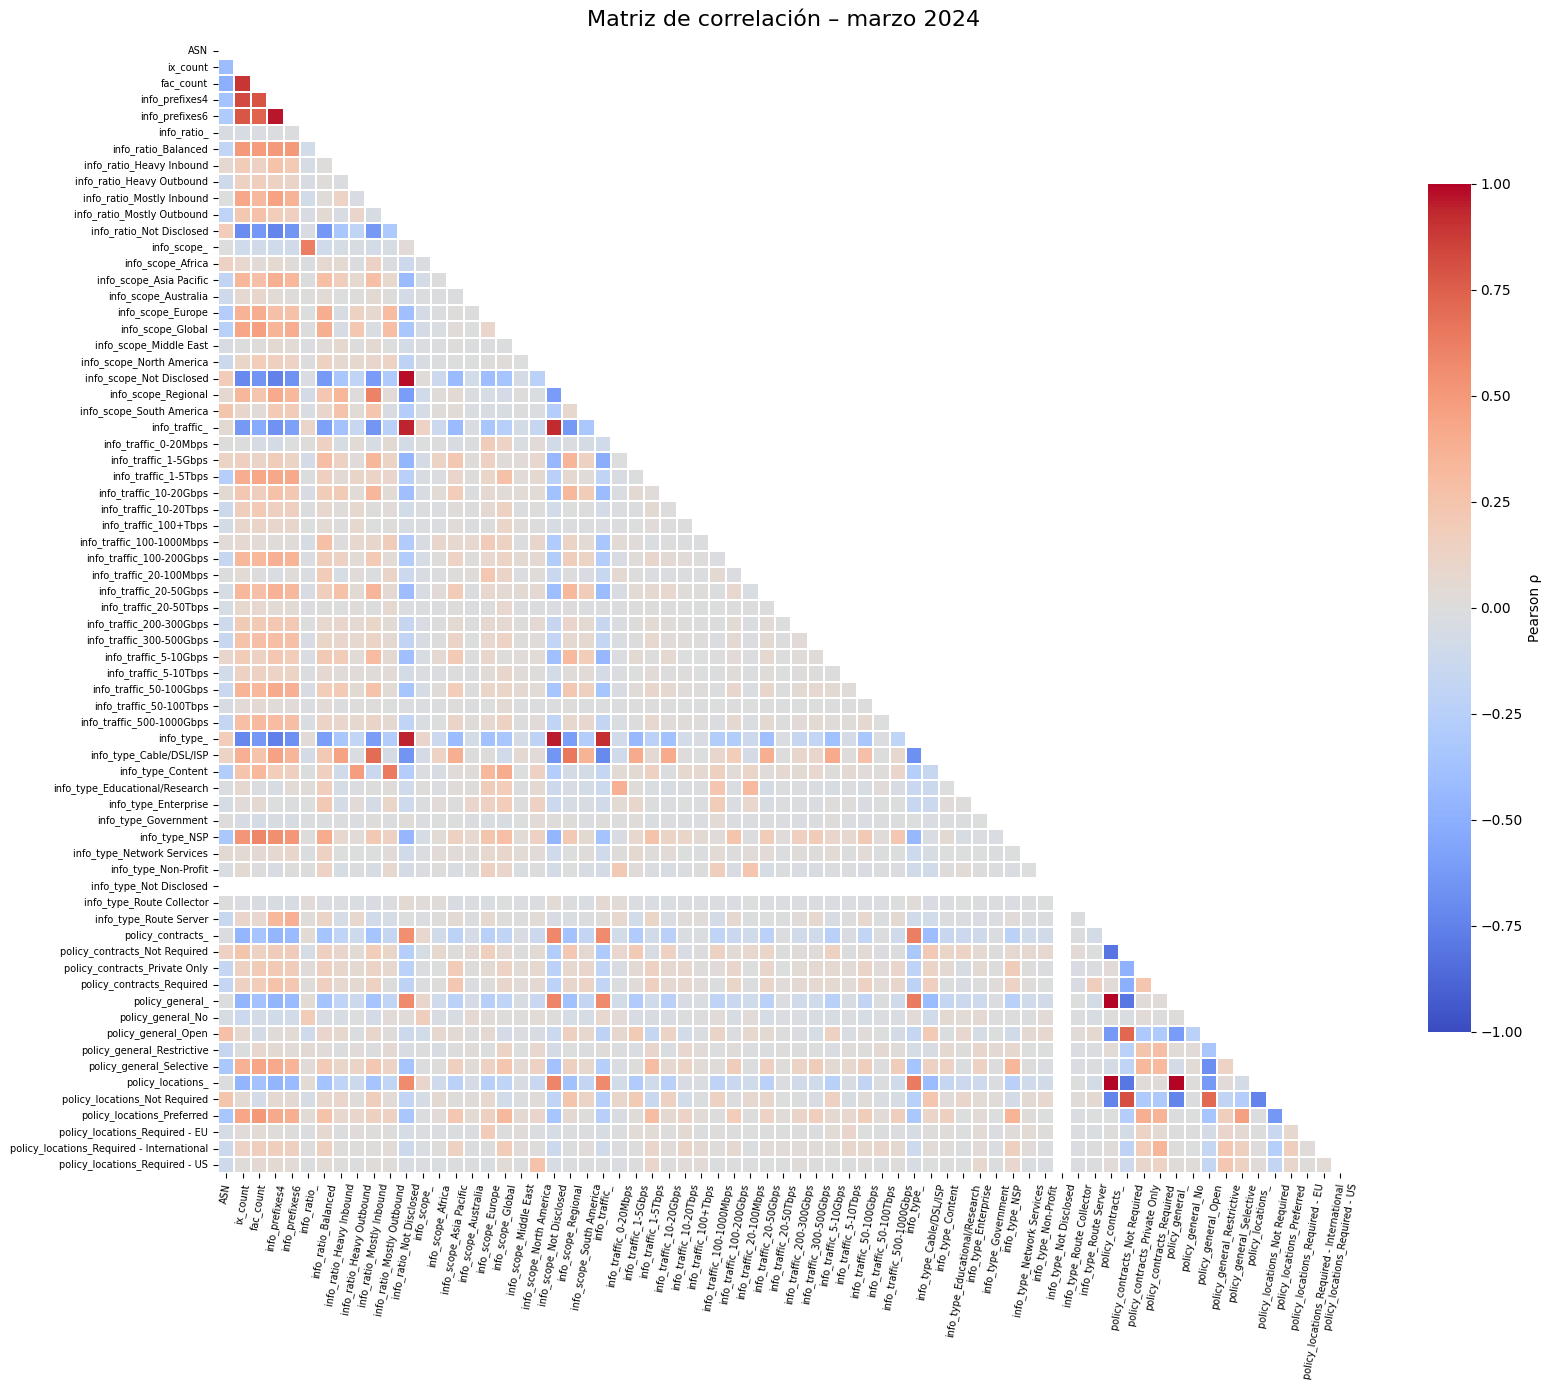
\includegraphics[width=\linewidth]{img/resultados/matriz_corr/matriz_corr_todos_attr.png}
%     \caption{Matriz de correlación de todos los atributos (febrero 2024).}
%     \label{fig:mat_corr_todos}
% \end{figure}

% Se calculó la matriz de correlación utilizando el coeficiente de Pearson. El valor en cada celda $\rho$ indica qué tan linealmente se relacionan dos variables, tomando valores entre $-1$ y $+1$. Para facilitar la visualización y el análisis, se extrajeron únicamente las correlaciones fuertes, es decir, aquellas donde $|\rho| \geq 0.5$.

% Se calculo la matriz de correlación usando el método de Pearson. Este valor en cada celda $\rho$ indica qué tan linealmente se relacionan dos variables. Una vez calculada y visualizada la matriz de correlación entre todos los atributos se quedo solo con las correlaciones fuertes tomando un umbral  $|\rho| \geq 0.5$, para una mejor visualización.


% \begin{figure}[H]
%     \centering
%     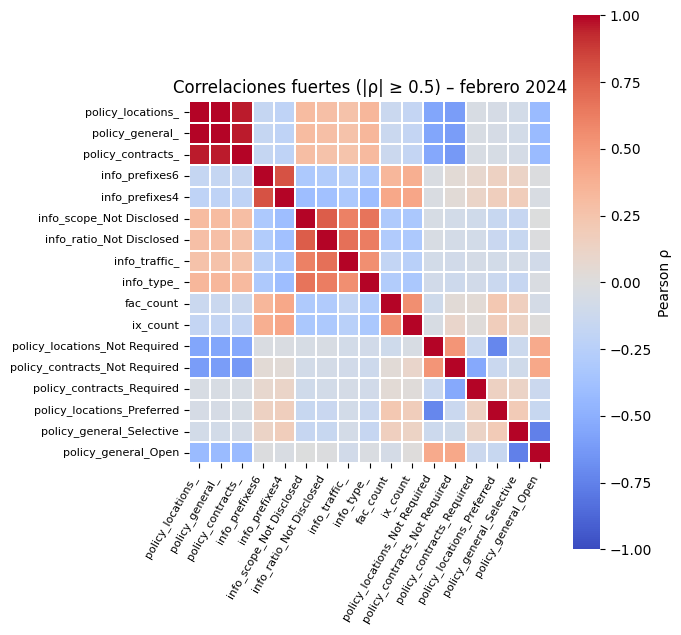
\includegraphics[width=0.65\linewidth]{img/resultados/matriz_corr/matriz_corr_febrero_altos.png}
%     \caption{Matriz de correlaciones fuertes ($|\rho| \geq 0.5$) entre atributos.}
%     \label{fig:mat_corr_fuerte}
% \end{figure}


% \paragraph{Interpretación de la matriz de atributos numéricos.}  
% En el mapa de calor, los colores indican la fuerza y dirección de la correlación:
% \begin{itemize}
%     \item Rojo intenso: correlación positiva fuerte.
%     \item Azul intenso: correlación negativa fuerte.
%     \item Celeste o gris claro: correlación débil o inexistente.
% \end{itemize}



% \begin{itemize}
%     \item \textbf{ix\_count/fac\_count:} los AS que aparecen en más IXPs suelen estar también presentes en más datacenters. Esto refleja que las redes grandes buscan mayor presencia física global.
%     \item \textbf{ix\_count/fac\_count – info\_prefixes4/6:} los AS con mayor conectividad física tienden a anunciar más bloques de direcciones IP (IPv4 e IPv6).
%     \item \textbf{info\_prefixes4 – info\_prefixes6:} presentan una correlación muy alta ($\rho > 0.80$), indicando que quienes anuncian muchos prefijos IPv4 también suelen anunciar muchos prefijos IPv6.
% \end{itemize}


% \begin{figure}[H]
%     \centering
%     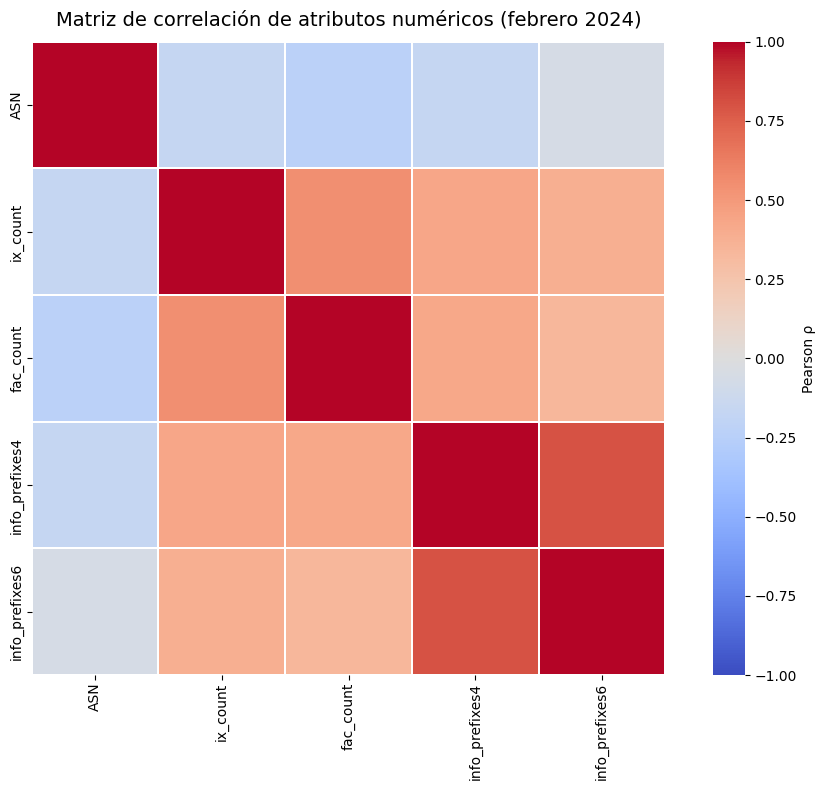
\includegraphics[width=0.6\linewidth]{img/resultados/matriz_corr/matriz_corr_attr_num.png}
%     \caption{Matriz de correlación entre atributos numéricos.}
%     \label{fig:mat_corr_numericos}
% \end{figure}




% %Esta informacion nos permite:
% %\begin{itemize}
% %    \item Optimizar el conjunto de atributos eliminando aquellos redundantes.
% %    \item Considerar la creación de indicadores agregados (por ejemplo, un índice de presencia global del AS).
% %    \item Asegurar que el modelo no se vea afectado por multicolinealidad, mejorando así su estabilidad y capacidad de generalización.
% %\end{itemize}


% %/////////////////////////////////////////////////////////////////
% \section{Análisis Embeddings Creados}

% \subsection{t-SNE}

% t-SNE es una técnica que “comprime” los vectores de alta dimensión (como tus embeddings) a sólo 2 dimensiones (o 3), tratando de preservar las distancias locales.\\

% Así, puedes visualizar en un gráfico plano cómo se agrupan, separan o mezclan los embeddings.

% Para visualizar si los embeddings que aprendió tu GNN tienen patrones interesantes:

%     ¿Los ASes similares están cerca?

%     ¿Se forman clusters claros?

%     ¿Las clases se separan en el espacio?

% Si ves grupos definidos o separaciones, normalmente es buena señal de que el embedding está “capturando” algo relevante



